\chapter{Resultados obtenidos}
	\label{sec:resultados}

	En este capítulo se muestran pruebas realizadas a la implementación del RNA y el ACG en diferentes casos de aplicación, que denominaremos \textit{ejemplos}. Estos ejemplos abarcan sistemas simples y complejos, desde ejemplos provistos por railML.org hasta sistemas reales, pasando por locaciones diseñadas por el autor de este trabajo para probar cada una de las funcionalidades del RNA y del ACG. En las siguientes secciones se analizará en detalle el primer ejemplo, lo que es suficiente para que el lector entienda el flujo de trabajo y los resultados obtenidos. Los ocho ejemplos restantes se encuentran en apéndices.
	
	En cada uno de los ejemplos se comparará el señalamiento obtenido mediante RNA, con el señalamiento de referencia para ese ejemplo. De esta forma será posible obtener conclusiones respecto a la eficacia del RNA, su impacto en la logística, seguridad y cobertura de la red. El análisis incluye la presentación de la topología original junto con su señalamiento y tabla de enclavamientos, siempre que esté disponible. Adicionalmente, se ilustrará la generación paso a paso del señalamiento, su simplificación y tabla de enclavamientos final, junto con la comparación con el enclavamiento original, si existiese. Finalmente, se incluyen las redes de grafos generadas por el RNA y un resumen de los recursos utilizados por el ACG para implementar el sistema.
	
	Alguno de los ejemplos que se usarán para probar los algoritmos fueron tomados de railML.Org u otras fuentes y se hará referencia a ellos como 'ejemplos tomados de railML', o bien se hará referencia a la fuente que corresponda, mientras que otros ejemplos que se usarán para probar los algoritmos fueron diseñados por el autor de esta tesis, y se hará referencia a ellos como 'ejemplos diseñados para las pruebas'. Cuando para el análisis se tome el señalamiento, sea el disponible en railML.Org o el diseñado por el autor, previo a ser procesador por el RNA se hablará de "señalamiento original", en el sentido de que se lo describirá previo a su procesamiento. En cambio, cuando para el análisis se tome el señalamiento producto de ser procesado por el RNA, se hablará de "señalamiento generado", ya que fue generado automáticamente por el RNA en base a la topología de la red ferroviaria.	
	
	\section{Plataforma utilizada}
	\label{sec:AGG}
	
	Cómo se explicó Sección \ref{sec:plataforma}, es posible utilizar una FPGA de cualquier fabricante, siempre y cuando tenga determinadas características de tamaño. En este contexto se optó por utilizar la FPGA ARTY Z7-20 de Xilinx (Figura \ref{fig:FPGA}) debido a cuestiones de disponibilidad y experiencia previa con la plataforma. La misma posee 53200 Look-up-tables, 106400 Flip-Flops, 32 Buffers y 125 bloque de entrada/salida. El precio promedio de esta plataforma ronda los 300 U\$D, un precio razonable para una plataforma de nivel intermedio.	
	
	\begin{figure}[H]
		\centering
		\includegraphics[width=1\textwidth]{Figuras/FPGA}
		\centering\caption{Plataforma FPGA Xilinx Arty Z7-20.}
		\label{fig:FPGA}
	\end{figure}
	
	Aunque se seleccionó una FPGA de la familia Xilinx \cite{Paper_30,Paper_36,Paper_37,Paper_40,Paper_41,Paper_47,Paper_97,Paper_104,Paper_106} y se utilizó el entorno de desarrollo integrado Vivado \cite{VIVADO,Paper_111}, por lo explicado en la Sección \ref{sec:plataforma}, el código VHDL generado por el ACG es independiente de la plataforma que se utilice. De emplearse otra familia de FPGAs, solo será necesaria una nueva asignación manual de pines de entrada y salida. De emplearse FPGAs por fuera de las familias ofrecidas por Xilinx, cómo por ejemplo Intel, puede utilizarse el entorno de desarrollo Intel Quartus \cite{QUARTUS}.
	
	Tanto el entorno de desarrollo Xilinx Vivado como el Intel Quartus incorporan herramientas para validación de la sintaxis generada por el ACG. Se utilizó la primera de ellas para generar el diagrama de bloques del sistema y analizar cada uno de los módulos y sus elementos internos. Este proceso incluye una validación de la sintaxis de todos los archivos generados por el ACG. Un análisis similar se realiza en las etapas de síntesis e implementación, detallado en profundidad en el Capítulo \ref{sec:resultados}.
	
	%La elección de una FPGA por sobre un microprocesador se debe a las ventajas expuestas en la Sección \ref{sec:FPGA} respecto a la concurrencia del sistema, mayor nivel de seguridad y facilidad para redundar el sistema. Además, los sistemas implementados en FPGA son considerados puramente hardware y no software, por lo que solamente deben cumplir los requerimientos de la norma EN 50129, especialmente el anexo F referido a FPGAs, y no la norma EN 50128 que se encarga del software. Los alcances de estas normas ya fueron explicados en la Sección \ref{sec:normas}.
	
	\section{Ejemplo 1}
  
    \subsection{Topología ferroviaria original}

El primer ejemplo, ilustrado en la Figura \ref{fig:EJ1_1}, es una topología diseñada en base a dos líneas principales y tres niveles de ramificaciones. La primera ramificación, utilizando el cambio de vías Sw06, es una ramificación simple. La segunda ramificación, utilizando el cambio de vías Sw04, es una ramificación compleja al incluir el cambio de vías Sw07 a continuación. Ademas, se incluyeron los cambios de vías Sw12 y Sw13 para permitir el intercambio de formaciones entre ambas vías principales. El objetivo de este ejemplo fue comprobar el funcionamiento del RNA con una topología de múltiples ramificaciones anidadas

\begin{figure}[h]
	\centering
	\includegraphics[width=1\textwidth]{resultados-obtenidos/ejemplo1/images/1_empty.png}
	\centering\caption{Topología ferroviaria del ejemplo 1 sin señalamiento.}
	\label{fig:EJ1_1}
\end{figure}

Para incrementar la dificultad del análisis y obtener resultados mas completos, se incluyeron finales de vías relativos y absolutos, junto con plataformas (Platform11, Platform13) y pasos a nivel (LevelCrossing6, Levelcrossing8). La infraestructura se distribuyó de forma tal de tener que en algunos casos el espacio entre ambos fuese suficiente (LevelCrossing 6 y Platform11) y en otros no (LevelCrossing8 y Platform13).
    \subsection{Señalamiento original}

    El señalamiento diseñado en forma manual por el autor de esta tesis para la topología de la Figura \ref{fig:EJ1_1} se ilustra en la Figura \ref{fig:EJ1_2}. Se observa que incluye señales de parada próximas a los finales de vías absolutos (S18, S19, S20), señales de partida en las plataformas (S04, S06, S08, S09), señales de protección antes de cada paso a nivel (S04, S05), señales de maniobras antes de converger en una vía principal (S03, S08) y señales múltiples para cambios de vías divergentes (S01, S17, S10, S07), entre varias otras señales. Estas señales permiten definir hasta un máximo de 14 rutas, todas ellas detalladas en la Tabla \ref{Tab:tabla_original_1}. En una primera inspección, se puede comprobar que todos los elementos ferroviarios son alcanzados por al menos una de las rutas, en al menos una dirección. Además, todos los cambios de vías son utilizados, de forma simple o compuesta. 
    
    \begin{figure}[H]
    	\centering
    	\includegraphics[width=1\textwidth]{resultados-obtenidos/ejemplo1/images/1_original.png}
    	\centering\caption{Señalamiento original del ejemplo 1.}
    	\label{fig:EJ1_2}
    \end{figure}
    
    \begin{table}[H]
        {
        \caption{Tabla de enclavamiento original del ejemplo 1.}
        \label{Tab:tabla_original_1}
        \centering
        \resizebox{1\textwidth}{!}{
            \begin{tabular}{ c c c c c c c }
                \hline	
                    Ruta & Inicio & Final & Cambio & Plataforma & Cruce & netElement \\	
                \hline
                    R$_{01}$  & S$_{05}$ & S$_{06}$ & - & Plat$_{11}$ & Lc$_{06}$ & ne$_{14}$\\
                    R$_{02}$  & S$_{06}$ & S$_{20}$ & - & - & - & ne$_{14}$\\
                    R$_{03}$  & S$_{09}$ & S$_{18}$ & - & - & - & ne$_{13}$\\
                    R$_{04}$  & S$_{13}$ & S$_{12}$ & Sw$_{13}^{N}$ & - & - & ne$_{23}$-ne$_{12}$\\
                    R$_{05}$  & S$_{16}$ & S$_{02}$ & Sw$_{12}^{N}$ & - & - & ne$_{22}$-ne$_{08}$\\
                    R$_{06}$  & S$_{07}$ & S$_{10}$ & Sw$_{06}^{N}$ & - & - & ne$_{02}$-ne$_{12}$\\
                    R$_{07}$  & S$_{07}$ & S$_{09}$ & Sw$_{06}^{R}$ & Plat$_{13}$ & Lc$_{08}$ & ne$_{02}$-ne$_{13}$\\
                    R$_{08}$  & S$_{10}$ & S$_{14}$ & Sw$_{13}^{N}$ & - & - & ne$_{12}$-ne$_{23}$\\
                    R$_{09}$  & S$_{10}$ & S$_{02}$ & Sw$_{12}^{R}$+Sw$_{13}^{R}$ & - & - & ne$_{12}$-ne$_{24}$-ne$_{08}$\\
                    R$_{10}$  & S$_{01}$ & S$_{17}$ & Sw$_{04}^{N}$ & - & - & ne$_{01}$-ne$_{08}$\\
                    R$_{11}$  & S$_{01}$ & S$_{19}$ & Sw$_{04}^{R}$+Sw$_{07}^{N}$ & - & - & ne$_{01}$-ne$_{15}$\\
                    R$_{12}$  & S$_{01}$ & S$_{05}$ & Sw$_{04}^{R}$+Sw$_{07}^{R}$ & - & - & ne$_{01}$-ne$_{14}$\\
                    R$_{13}$  & S$_{17}$ & S$_{15}$ & Sw$_{12}^{N}$ & - & - & ne$_{08}$-ne$_{22}$\\
                    R$_{14}$  & S$_{17}$ & S$_{12}$ & Sw$_{12}^{R}$+Sw$_{13}^{R}$ & - & - & ne$_{08}$-ne$_{24}$-ne$_{12}$\\    
                \hline
            \end{tabular}
        }
     }
    \end{table}
    
    Algunas rutas abarcan mas de un \textit{netElement}, como por ejemplo la ruta R14 que comienza en la señal S17 y finaliza en la señal S12, atraviesa los \textit{netElements} ne8, ne24 y ne12, y utiliza los cambios de vías Sw12 y Sw13, ambos en posición reversa.

    \subsection{Generación de señalamiento paso a paso}

	Al ejecutar el RNA, primero detectará todos los \textit{netElements}, sus coordenadas iniciales y finales en la topología, y el sentido en el que fueron definidas. El resultado obtenido se muestra en el Cóodigo \ref{lst:EJ1_1}.
	
	\begin{lstlisting}[language = {}, caption = Detección de \textit{netElements} por parte del RNA , label = {lst:EJ1_1}]
		###### Starting Railway Network Analyzer #####
		Reading .railML file
		Creating railML object
		Analysing railML object
		Analysing graph
		ne1 [810, 150] [1320, 150] >>
		ne2 [2970, 0] [2460, 0] <<
		ne8 [1320, 150] [1800, 150] >>
		ne9 [1320, 150] [1530, 360] >>
		ne12 [2460, 0] [1950, 0] <<
		ne13 [2460, 0] [810, -180] <<
		ne14 [1530, 360] [2970, 360] >>
		ne15 [1530, 360] [2970, 570] >>
		ne22 [1800, 150] [2970, 150] >>
		ne23 [1950, 0] [810, 0] <<
		ne24 [1800, 150] [1950, 0] >>
		The network is connected
	\end{lstlisting}
	
	Por ejemplo, el \textit{netElement} ne1 inicia en la coordenada (810;150) y finaliza en la coordenada (1320;150). El símbolo $>>$ indica que ne1 se encuentra definido de izquierda a derecha, ya que la componente x de cada la coordenada final es mayor al de la coordenada inicial, teniendo la misma componente y. Además, se puede comprobar que la lista obtenida en consistente con la Figura \ref{fig:EJ1_2}. Por ejemplo, ne1, ne8 y ne9 comparten la coordenada (1320;150), que coincide con la coordenada del cambio de vías Sw04.
	
	A continuación, el RNA detectará la infraestructura ferroviaria, las curvas peligrosas y los puntos medios de los netElements que el RNA considera demasiado largos. El resultado de este proceso se puede visualizar en el Código \ref{lst:EJ1_2} y puede leerse también en el archivo Infrastructure.RNA.
	
	\begin{lstlisting}[language = {}, caption = Detección de puntos críticos por parte del RNA , label = {lst:EJ1_3}]
		Analysing infrastructure --> Infrastructure.RNA
		Detecting Danger --> Safe_points.RNA
		ne1 has a Middle point @ [1065.0, 150]
		ne2 has a Middle point @ [2715.0, 0]
		ne8 has a Middle point @ [1560.0, 150]
		ne12 has a Middle point @ [2205.0, 0]
		ne13 has a Platform[plf75] @ [1564, 180]
		ne13 has a LevelCrossing[lcr74] @ [1362, 180]
		ne13 has a Curve(2 lines) @ [[2280, -180]]
		ne14 has a Platform[plf68] @ [2490, -360]
		ne14 has a LevelCrossing[lcr69] @ [1945, -360]
		ne15 has a Curve(2 lines) @ [[1740, 570]]
		ne22 has a RailJoint[J15] @ [2452, 150]
		ne23 has a RailJoint[J14] @ [1284, 0]
	\end{lstlisting}
	
	Una vez que el RNA detectó cada punto crítico de la red ferroviaria, procede a generar el señalamiento. El orden de generación no es importante, pero para poder describirlo de forma consistente se iniciará generando el señalamiento para proteger los finales de vías, las junturas entre rieles, las plataformas, los cruces de vía y los cambios de vías. Luego se procederá a mostrar el señalamiento pre y post simplificación. Las señales generadas para proteger los finales de vías relativos y absolutos son ilustradas en la Figura \ref{fig:EJ1_3}.
	
	\begin{figure}[H]
		\centering
		\includegraphics[width=1\textwidth]{resultados-obtenidos/ejemplo1/images/1_step1.png}
		\centering\caption{Señalamiento generado por el RNA para proteger el fin de vía.}
		\label{fig:EJ1_3}
	\end{figure}
	
	Los finales de vías absolutos son protegidos por las señales de parada T01, T03, T05 y las señales de partida son T02, T04 y T06. A su vez, los finales de vías relativos poseen las señales de parada L07, L08, L09 y L10, cercanos al límite del externo del \textit{netElement} al que pertenecen.
	
	La Figura \ref{fig:EJ1_3} ilustra la generación de señales destinadas a proteger las junturas entre los rieles. Las señales generadas son J11, J12, J13 y J14, indicadas en color rojo. De no existir junturas que proteger, el RNA salteará este paso.
	
	\begin{figure}[H]
		\centering
		\includegraphics[width=1\textwidth]{resultados-obtenidos/ejemplo1/images/1_step2.png}
		\centering\caption{Señalamiento generado por el RNA para proteger las junturas.}
		\label{fig:EJ1_4}
	\end{figure}
	
	Al generar el señalamiento para proteger las, tal como se explicó en la Sección \ref{sec:horizontal}, el Algoritmo 	\ref{alg:horizontal} simplificará las señales entre dos elementos ferroviarios si no existe espacio suficiente entre ellos, tal como sucede con los elementos levelCrossing8 y Platform13. El señalamiento generado para proteger las plataformas y los cruces de vía se ilustra en rojo en la Figura \ref{fig:EJ1_5}. Las señales generadas para proteger las plataformas son las señales de partida P18, P19 y P20, mientras que las señales que protegen los cruces de vía son las señales X15, X16 y X17.
		
	\begin{figure}[H]
		\centering
		\includegraphics[width=1\textwidth]{resultados-obtenidos/ejemplo1/images/1_step3.png}
		\centering\caption{Señalamiento generado por el RNA para proteger plataformas y cruces de vía.}
		\label{fig:EJ1_5}
	\end{figure}
	
	El RNA generó las señales S22, C21, H23 y H24 para proteger el cambio de vías Sw04; las señales S27, C25, B26 y H28 para proteger el cambio de vías Sw06; las señales C29 y B30 para proteger el cambio de vías Sw07; las señales S32, C31 y H33 para proteger el cambio de vías Sw12 y las señales S35, C34 y H36 para proteger el cambio de vías Sw13. Las señales mencionadas se encuentran resaltadas en rojo en la Figura \ref{fig:EJ1_6}.
	
	\begin{figure}[H]
		\centering
		\includegraphics[width=1\textwidth]{resultados-obtenidos/ejemplo1/images/1_step4.png}
		\centering\caption{Señalamiento generado por el RNA para proteger los cambios de vías.}
		\label{fig:EJ1_6}
	\end{figure}
	
	Una vez obtenido todo el señalamiento, el RNA procede a simplificar las señales redundantes, repetidas o cuyas funciones o ubicaciones se superponen entre sí. El proceso de simplificación de señales fue explicado en la Sección \label{sec:simplificacion}. El Algoritmo \ref{alg:vertical} de herencia vertical fue aplicado en las señales B entre los cambios de vías Sw12 y Sw13, desplazando las señales hasta convertirlas en las señales H33 y H36 respectivamente. Análogamente, las señales C y S del \textit{netElement} se convirtieron en las señales H23 y H24 respectivamente.
	
	Las señales simplificadas al aplicar el Algoritmo \ref{alg:horizontal} de herencia horizontal son: X17, P18, P19, B26, B30, C31 y C34. Las señales X17 y B26 fueron eliminadas por su cercanía con la señal T02, con la cual comparten dirección y sentido. Lo mismo ocurre entre el par de señales P18/B30 y la señal T04; entre las señales P19 y T03; entre las señales C31 y J12; y entre las señales C34 y J13. En todos los casos, se aplicó el Algoritmo \ref{alg:horizontal}, diseñado para agrupar objetos cercanos como un único objeto, generando el señalamiento acorde a los elementos contenidos en cada extremo del nuevo elemento contenedor.
	
	Finalmente, las señales son simplificadas aplicando el Algoritmo \ref{alg:reduction} de eliminación por prioridad de señales. El resultado de este proceso es detallado en el Código \ref{lst:EJ1_4}.
	
	\begin{lstlisting}[language = {}, caption = Reducción de señalamiento por prioridad de señales, label = {lst:EJ1_4}]
		Reducing redundant signals
		removing sig17 for sig02
		removing sig26 for sig02
		removing sig19 for sig03
		removing sig30 for sig04
		removing sig31 for sig12
		removing sig34 for sig13
		removing sig18 for sig30
	\end{lstlisting}
	
	El resultado de la simplificación del señalamiento se ilustra en la Figura \ref{fig:EJ1_7}.
	
	\begin{figure}[H]
		\centering
		\includegraphics[width=1\textwidth]{resultados-obtenidos/ejemplo1/images/1_RNA.png}
		\centering\caption{Señalamiento generado y simplificado por el RNA.}
		\label{fig:EJ1_7}
	\end{figure}
	
	\lipsum[1]
	
	% ARCHIVOS RNA GENERADOS
	
	
	
	
	
	
	
	
	
	
    \subsection{Red de grafos generada por el RNA}

 \lipsum[1]

\begin{figure}[H]
	\centering
	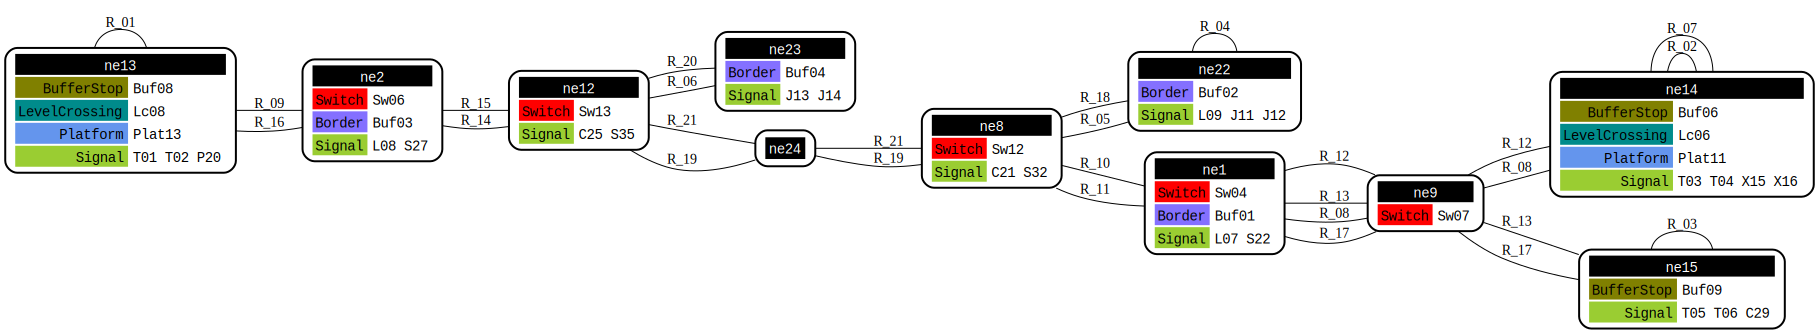
\includegraphics[angle = 90, origin = c, width=0.29\textwidth]{Figuras/Graph_1}
	\centering\caption{XXXX}
	%\label{fig:LC_P2}
\end{figure}

\lipsum[1]
    \subsection{Señalamiento generado por el RNA}

    El RNA también exporta la información mostrada en el Código \ref{lst:EJ1_8} en una hoja de cálculo, similar a la que se visualiza en la Tabla \ref{Tab:tabla_generated_1}.
    
    \begin{table}[H]
        {
        \caption{Tabla de enclavamiento del ejemplo 1 generada por el RNA.}
        \label{Tab:tabla_generated_1}
        \centering
        \resizebox{1\textwidth}{!}{
            \begin{tabular}{ c c c c c c c }
                \hline	
                    Ruta & Inicio & Final & Cambio & Plataforma & Cruce & netElement \\	
                \hline
                    R$_{01}$  & T$_{02}$ & P$_{20}$ & - & Plat$_{13}$ & Lc$_{08}$ & ne$_{13}$\\
                    R$_{02}$  & T$_{04}$ & X$_{16}$ & - & Plat$_{11}$ & - & ne$_{14}$\\
                    R$_{03}$  & T$_{06}$ & C$_{29}$ & - & - & - & ne$_{15}$\\
                    R$_{04}$  & J$_{11}$ & L$_{09}$ & - & - & - & ne$_{22}$\\
                    R$_{05}$  & J$_{12}$ & C$_{21}$ & Sw$_{12}^{N}$ & - & - & ne$_{22}$-ne$_{08}$\\
                    R$_{06}$  & J$_{13}$ & C$_{25}$ & Sw$_{13}^{N}$ & - & Lc$_{08}$ & ne$_{23}$-ne$_{12}$\\
                    R$_{07}$  & X$_{15}$ & T$_{03}$ & - & Plat$_{11}$ & Lc$_{06}$ & ne$_{14}$\\
                    R$_{08}$  & X$_{16}$ & L$_{07}$ & Sw$_{04}^{R}$+Sw$_{07}^{R}$ & - & - & ne$_{14}$-ne$_{01}$\\
                    R$_{09}$  & P$_{20}$ & L$_{08}$ & Sw$_{06}^{R}$ & - & - & ne$_{13}$-ne$_{02}$\\
                    R$_{10}$  & C$_{21}$ & L$_{07}$ & Sw$_{04}^{N}$ & - & - & ne$_{08}$-ne$_{01}$\\
                    R$_{11}$  & S$_{22}$ & S$_{32}$ & Sw$_{04}^{N}$ & - & - & ne$_{01}$-ne$_{08}$\\
                    R$_{12}$  & S$_{22}$ & X$_{15}$ & Sw$_{04}^{R}$+Sw$_{07}^{R}$ & - & - & ne$_{01}$-ne$_{14}$\\
                    R$_{13}$  & S$_{22}$ & T$_{05}$ & Sw$_{04}^{R}$+Sw$_{07}^{N}$ & - & - & ne$_{01}$-ne$_{15}$\\
                    R$_{14}$  & C$_{25}$ & L$_{08}$ & Sw$_{06}^{N}$ & - & - & ne$_{12}$-ne$_{02}$\\
                    R$_{15}$  & S$_{27}$ & S$_{35}$ & Sw$_{06}^{N}$ & - & - & ne$_{02}$-ne$_{12}$\\
                    R$_{16}$  & S$_{27}$ & T$_{01}$ & Sw$_{06}^{R}$ & Plat$_{13}$ & Lc$_{08}$ & ne$_{02}$-ne$_{13}$\\
                    R$_{17}$  & C$_{29}$ & L$_{07}$ & Sw$_{04}^{R}$+Sw$_{07}^{N}$ & - & - & ne$_{15}$-ne$_{01}$\\
                    R$_{18}$  & S$_{32}$ & J$_{11}$ & Sw$_{12}^{N}$ & - & - & ne$_{08}$-ne$_{22}$\\
                    R$_{19}$  & S$_{32}$ & C$_{25}$ & Sw$_{12}^{R}$+Sw$_{13}^{R}$ & - & - & ne$_{08}$-ne$_{12}$\\
                    R$_{20}$  & S$_{35}$ & J$_{14}$ & Sw$_{13}^{N}$ & - & - & ne$_{12}$-ne$_{23}$\\
                    R$_{21}$  & S$_{35}$ & C$_{21}$ & Sw$_{12}^{R}$+Sw$_{13}^{R}$ & - & - & ne$_{12}$-ne$_{08}$\\
                \hline
            \end{tabular}
        }
     }
    \end{table}
    
    En una primera inspección podemos ver que el nuevo señalamiento tiene 21 rutas, versus las 14 rutas del señalamiento original (ver Tabla \ref{Tab:tabla_original_1}). Esto se debe a que todas las vías son consideradas de ambos sentidos por el RNA, lo cuál queda de manifiesto cuando se comprueba que todas las plataformas y cruces de vía son atravesados por dos rutas, una en cada dirección. 
    \subsection{Validacion del sistema}

    \lipsum[1]

    \begin{table}[!h]
        {
        \caption{Equivalencias entre las rutas originales y las generadas por el RNA.}
        \label{Tab:tabla_validation_1}
        \centering
        %\small
            %\centering
            \begin{center}
            \resizebox{1\textwidth}{!}{
            \begin{tabular}{ c c c c }
                \hline	
                    Original & Señales & RNA & Señales \\	
                \hline
                    R$_{01}$ & S$_{05}$-S$_{06}$ & R$_{07}$ & X$_{15}$-T$_{03}$ \\
                    R$_{02}$ & S$_{06}$-S$_{20}$ & R$_{07}$ & X$_{15}$-T$_{03}$ \\
                    R$_{03}$ & S$_{09}$-S$_{18}$ & R$_{16}$ & S$_{27}$-T$_{01}$ \\
                    R$_{04}$ & S$_{13}$-S$_{12}$ & R$_{06}$ & J$_{13}$-C$_{25}$ \\
                    R$_{05}$ & S$_{16}$-S$_{02}$ & R$_{05}$ & J$_{12}$-C$_{21}$ \\
                    R$_{06}$ & S$_{07}$-S$_{10}$ & R$_{15}$ & S$_{27}$-S$_{35}$ \\
                    R$_{07}$ & S$_{07}$-S$_{09}$ & R$_{16}$ & S$_{27}$-T$_{01}$ \\
                    R$_{08}$ & S$_{10}$-S$_{14}$ & R$_{20}$ & S$_{35}$-J$_{14}$ \\
                    R$_{09}$ & S$_{10}$-S$_{02}$ & R$_{21}$ & S$_{35}$-C$_{21}$ \\
                    R$_{10}$ & S$_{01}$-S$_{17}$ & R$_{11}$ & S$_{22}$-S$_{32}$ \\
                    R$_{11}$ & S$_{01}$-S$_{19}$ & R$_{13}$ & S$_{22}$-X$_{15}$ \\
                    R$_{12}$ & S$_{01}$-S$_{05}$ & R$_{12}$ & S$_{22}$-T$_{05}$ \\
                    R$_{13}$ & S$_{17}$-S$_{15}$ & R$_{18}$ & S$_{32}$-J$_{11}$ \\
                    R$_{14}$ & S$_{17}$-S$_{12}$ & R$_{19}$ & S$_{32}$-C$_{25}$ \\   
                \hline
            \end{tabular}
            }
            \end{center}
        }    
    \end{table}
    \subsection{Sistema generado por el ACG}
	\label{sec:EJEMPLO1_ACG}
	
	En base a la red de grafos, ilustrada en la Figura \ref{fig:EJ1_8}, el ACG determinó la cantidad de elementos ferroviarios de cada tipo, tal como puede visualizarse en el Código \ref{lst:EJ1_8}.
	
	\begin{lstlisting}[language = {}, caption = Cantidad de elementos a implementar por el ACG, label = {lst:EJ1_8}]
	n_netElements:11
	n_switch:5
	n_doubleSwitch:0
	n_borders:4
	n_buffers:3
	n_levelCrossings:2
	n_platforms:2
	n_scissorCrossings:0
	n_signals:23
	N : 62
	\end{lstlisting}
	
	El ACG genera, en el caso de este ejemplo, 80 archivos en formato VHDL, tal como se puede visualizar en la Figura \ref{fig:EJ1_ACG_1}. Podemos destacar de la Figura \ref{fig:EJ1_ACG_1} al archivo \textit{Arty\_Z7-10.XDCxdc}, el primero arriba a la izquierda, que define los pines de entrada y salida de la plataforma Arty Z7 10 y Arty Z7 20. Este archivo es provisto por Xilinx para esta familia de plataformas. En caso de utilizar otra plataforma de Xilinx, se deberá incluir el archivo XDC correspondiente. En ambos casos, cada desarrollador debe asignar manualmente los pines a cada puerto del sistema generado por el ACG.
	
	\begin{figure}[H]
		\centering
		\includegraphics[origin = c, width=1\textwidth]{resultados-obtenidos/ejemplo1/images/ACG_files}
		\centering\caption{Archivos generador por el ACG para el ejemplo 1.}
		\label{fig:EJ1_ACG_1}
	\end{figure}
	
	Además, se pueden mencionar los archivos \textit{my\_package.vhdl} y \textit{flipFlop.vhdl}, ambos generados por el ACG. El primero es una librería que define todos los tipos de datos utilizados por el sistema, y el segundo es un flip-flop tipo D utilizado para generar la secuencia de shift registers necesarios para adaptar el clock de entrada a los diferentes dominios de clock necesarios para el timeout de cada elemento ferroviario.
	
	Los archivos restantes son archivos que definen los módulos de alto nivel explicados en la Sección \ref{sec:interlockingArch} o la representación en VHDL de cada elemento ferroviario explicada entre la Sección \ref{sec:ACG_lc} y la Sección \ref{sec:ACG_rts}. Por ejemplo, en base lo descrito en el Código \ref{lst:EJ1_8}, hay 23 señales ferroviarias y podemos visualizar en la Figura \ref{fig:EJ1_ACG_1} 23 archivos referidos a las señales ferroviarias: desde \textit{railwaySignal\_0} hasta \textit{railwaySignal\_22}. Un ejemplo de la complejidad y profundidad del código generado es el archivo \textit{route\_13} (que corresponde a la ruta 13 de la Tabla \ref{Tab:tabla_generated_1}) que se puede visualizar en el Código \ref{lst:EJ1_vhdl}.	El Código \ref{lst:EJ1_vhdl} incluye la declaración de puertos, la creación de las variables necesarias, la conversión de tipos de datos, la conexión de flip-flops para generar un shift-register tal que se puedan utilizar como timeout con las condiciones prefijadas y la máquina de estados de la ruta 13, tal como se explicó en la Sección \ref{sec:ACG_rts}.
	
	\begin{lstlisting}[language = {vhdl}, caption = route\_13.vdhl, label = {lst:EJ1_vhdl}, tabsize=2, basicstyle=\footnotesize\ttfamily]
--  route_13.vhdl : Automatically generated using ACG
	library IEEE;
	use IEEE.std_logic_1164.all;
	use IEEE.numeric_std.all;
	library work;
--Declare the package
	use work.my_package.all;
	entity route_13 is
	port(
		clock : in std_logic := '0';
		reset : in std_logic := '0';
		routeRequest : in hex_char;
		track_ne12 : in hex_char;
		ne12_command : out routeCommands := RELEASE;
		track_ne2 : in hex_char;
		ne2_command : out routeCommands := RELEASE;
		Sw06_state : in hex_char;
		Sw06_command : out routeCommands := RELEASE;
		C25_state : in hex_char;
		C25_command : out routeCommands := RELEASE;
		L08_state : in hex_char;
		L08_command : out routeCommands := RELEASE;
		routeExecute : out hex_char
	);
	end entity route_13;
	
	architecture Behavioral of route_13 is
		component flipFlop is
		port(
			clock : in std_logic := '0';
			reset : in std_logic := '0';
			Q : out std_logic := '0'
		);
		end component flipFlop;
	signal restart : std_logic := '1';
	signal Q : std_logic_vector(32 downto 0) := (others => '0');
	signal clock_in : std_logic_vector(32 downto 0) := (others => '0');
	signal timeout : std_logic := '0';
	signal routeState : routeStates := WAITING_COMMAND;
	signal routingIn : routeStates;
	signal ne12_used , ne2_used : std_logic := '0';
	signal ne12_state : nodeStates := FREE;
	signal ne12_lock : objectLock := RELEASED;
	signal ne2_state : nodeStates := FREE;
	signal ne2_lock : objectLock := RELEASED;
	signal Sw06_position : singleSwitchStates := NORMAL;
	signal Sw06_lock : objectLock := RELEASED;
	signal C25_aspectIn : signalStates := RED;
	signal C25_lock: objectLock := RELEASED;
	signal L08_aspectIn : signalStates := RED;
	signal L08_lock : objectLock := RELEASED;
	begin
		clock_in(0) <= clock;
		routingIn <= routeStates'val(to_integer(unsigned(hex_to_slv(routeRequest))));
		routeExecute <= slv_to_hex(std_logic_vector(to_unsigned(routeStates'pos(routeState),4)));
		ne12_state <= nodeStates'val(to_integer(unsigned(hex_to_slv(track_ne12)(2 to 3))));
		ne12_lock <= objectLock'val(to_integer(unsigned(hex_to_slv(track_ne12)(0 to 1))));
		ne2_state <= nodeStates'val(to_integer(unsigned(hex_to_slv(track_ne2)(2 to 3))));
		ne2_lock <= objectLock'val(to_integer(unsigned(hex_to_slv(track_ne2)(0 to 1))));
		Sw06_position <= singleSwitchStates'val(to_integer(unsigned(hex_to_slv(Sw06_state)(2 to 3))));
		Sw06_lock <= objectLock'val(to_integer(unsigned(hex_to_slv(Sw06_state)(0 to 1))));
		C25_aspectIn <= signalStates'val(to_integer(unsigned(hex_to_slv(C25_state)(2 to 3))));
		C25_lock <= objectLock'val(to_integer(unsigned(hex_to_slv(C25_state)(0 to 1))));
		L08_aspectIn <= signalStates'val(to_integer(unsigned(hex_to_slv(L08_state)(2 to 3))));
		L08_lock <= objectLock'val(to_integer(unsigned(hex_to_slv(L08_state)(0 to 1))));
	
		gen : for i in 0 to 31 generate
			inst: flipFlop port map(clock_in(i), restart, Q(i));
			clock_in(i+1) <= Q(i);
		end generate;
	
		process(clock,reset,Q,restart)
		begin
			if (reset = '1' or Q = "011011111100001000111010101111110") then
				timeout <= '1';
			end if;
			if (restart = '1') then
				timeout <= '0';
			end if;
		end process;
		
		process(clock)
		begin
			if (clock'Event and clock = '1') then
				case routeState is
					when WAITING_COMMAND =>
					if (routingIn = ROUTE_REQUEST) then
						routeState <= RESERVING_TRACKS;
					end if;
					when RESERVING_TRACKS =>
						restart <= '0';
						if (routingIn = CANCEL_ROUTE or timeout ='1') then
							routeState <= CANCEL_ROUTE;
						end if;
						if ((ne12_lock = RELEASED and ne2_lock = RELEASED) and (ne2_state = FREE)) then
							ne12_command <= RESERVE;
							ne2_command <= RESERVE;
						end if;
						if (ne12_lock = RESERVED and ne2_lock = RESERVED)then
							restart <= '1';
							routeState <= LOCKING_TRACKS;
						end if;
			when LOCKING_TRACKS =>
				restart <= '0';
				if (routingIn = CANCEL_ROUTE or timeout ='1') then
					routeState <= CANCEL_ROUTE;
				end if;
				if ((ne12_lock = RESERVED and ne2_lock = RESERVED) and (ne2_state = FREE)) then
					ne12_command <= LOCK;
					ne2_command <= LOCK;
				end if;
				if (ne12_lock = LOCKED and ne2_lock = LOCKED)then
					restart <= '1';
					routeState <= RESERVING_INFRASTRUCTURE;
				end if;
			when RESERVING_INFRASTRUCTURE =>
				restart <= '0';
				if (routingIn = CANCEL_ROUTE or timeout ='1') then
					routeState <= CANCEL_ROUTE;
				end if;
				if (Sw06_lock = RELEASED) then
					Sw06_command <= RESERVE;
				end if;
				if (Sw06_lock = RESERVED)then
					restart <= '1';
					routeState <= LOCKING_INFRASTRUCTURE;
				end if;
			when LOCKING_INFRASTRUCTURE =>
				restart <= '0';
				if (routingIn = CANCEL_ROUTE or timeout ='1') then
					routeState <= CANCEL_ROUTE;
				end if;
				if (Sw06_lock = RESERVED) then
					Sw06_command <= LOCK;
				end if;
				if (Sw06_lock = LOCKED)then
					ne12_used <= '0';
					ne2_used <= '0';
					restart <= '1';
					routeState <= DRIVING_SIGNAL;
				end if;
			when DRIVING_SIGNAL =>
				restart <= '0';
				if (routingIn = CANCEL_ROUTE or timeout ='1') then
					routeState <= CANCEL_ROUTE;
				end if;
				if (C25_lock = RELEASED and L08_lock = RELEASED) then
					C25_command <= RESERVE;
					L08_command <= LOCK;
				end if;
				if (C25_lock = RESERVED and L08_lock = LOCKED) then
					restart <= '1';
					routeState <= SEQUENTIAL_RELEASE;
				end if;
			when SEQUENTIAL_RELEASE =>
				restart <= '0';
				if (routingIn = CANCEL_ROUTE or timeout ='1') then
					routeState <= CANCEL_ROUTE;
				end if;
				--- Sequential release
				if (ne12_used = '0' and ne12_state = OCCUPIED) then 
					ne12_used <= '1';
				end if;
				if (ne12_used = '1' and ne12_state = FREE) then
					ne12_used <= '0';
					ne12_command <= RELEASE;
				end if;
				---
				if (ne12_lock = RELEASED and ne2_used = '0' and ne2_state = OCCUPIED) then 
					ne2_used <= '1';
					--- Finish -> Release all
					restart <= '1';
					routeState <= RELEASING_INFRASTRUCTURE;
				end if;
			when RELEASING_INFRASTRUCTURE =>
				Sw06_command <= RELEASE;
				ne12_command <= RELEASE;
				ne2_command <= RELEASE;
				C25_command <= RELEASE;
				L08_command <= RELEASE;
				restart <= '1';
				routeState <= WAITING_COMMAND;
			when CANCEL_ROUTE =>
				routeState <= RELEASING_INFRASTRUCTURE;
			when others =>
				routeState <= WAITING_COMMAND;
			end case;
		end if;
		end process;
	end Behavioral;
	\end{lstlisting}
	
	
	Cada ejemplo cuenta con su propia carpeta de principio a fin. Estas carpetas contienen el archivo railML original, los archivos generados por el RNA y el código generado por el ACG. Esto es una ventaja a la hora de mantener un orden pero una gran desventaja a la hora de sintetizar los proyectos en Vivado. Cada conjunto de archivos debería ser importado de manera individual, previa desvinculación de los archivos del proyecto anterior. Para solucionar este inconveniente se desarrolló el Código \ref{lst:EJ1_script}, implementado en el lenguaje de scripting TCL (Tool Command Language), que automatiza la importación y desvinculación de los archivos de cada ejemplo.
	
	\begin{lstlisting}[language = {bash}, caption = script.tcl, label = {lst:EJ1_script}]
set chosen 1

# Get a list of all design source files
set design_sources [get_files -of_objects [get_filesets sources_1]]

remove_files $design_sources

set base_folder_path "ROOT/GICSAFePhD/App/Layouts/Example_"
set folder_path "${base_folder_path}${chosen}/VHDL"

puts $folder_path

set files [glob -directory $folder_path *.vhd]

add_files -norecurse -scan_for_includes  $files

update_compile_order -fileset sources_1
update_compile_order -fileset sources_1

synth_design -rtl -rtl_skip_mlo -name rtl_1
	\end{lstlisting}
	
	El parámetro \textit{chosen} (línea 1) indica el número de ejemplo seleccionado, mientras que \textit{base\_folder\_path} (línea 8) es la ruta absoluta de los ejemplos, cuyas carpetas deben ser nombradas como \textit{Example\_}+\textit{chosen} para poder ser encontradas. El Código \ref{lst:EJ1_script} puede ser importado en Vivado desde \textit{Tools $>$ Custom Commands $>$ Customize Commands} como un archivo TCL (del inglés, Tool Command Language), que es el formato que define los comandos nativos de Vivado. Pueden importarse tantos archivos TCL como se deseen, uno por cada ejemplo a sintetizar. De esta manera, cada script aparecerá en la barra de acceso rápido de Vivado de forma independiente y se automatiza el proceso de sincronización de archivos.
	
	Una vez ejecutado el script, Vivado ordenará los archivos de forma jerárquica, como puede verse en la parte izquierda de la Figura \ref{fig:EJ1_ACG_Vivado}, que para comodidad del lector se muestra en forma ampliada en la Figura \ref{fig:EJ1_ACG_Vivado_ampliado}, donde el módulo \textit{global} incluye todos los módulos que fueron detallados en la Sección \ref{sec:interlockingArch}. Se puede destacar al módulo \textit{network} que es instanciado 3 veces junto con el módulo \textit{voter}, al ser una redundancia 2oo3, tal fue explicado en la Sección \ref{sec:network}. Cada una de las instancias del módulo \textit{network} contienen sus propias 62 instancias de los mismos módulos de cada elemento ferroviario ya que N, cantidad de elementos ferroviarios, es 62 en el Código \ref{lst:EJ1_8}.	
	
	\begin{figure}[H]
		\centering
		\includegraphics[origin = c, width=1\textwidth]{resultados-obtenidos/ejemplo1/images/ACG_vivado}
		\centering\caption{Interfaz del entorno de desarrollo Vivado para el ejemplo 1.}
		\label{fig:EJ1_ACG_Vivado}
	\end{figure}
	
	\begin{figure}[H]
		\centering
		\includegraphics[origin = c, width=0.85\textwidth]{resultados-obtenidos/ejemplo1/images/ACG_vivado_2}
		\centering\caption{Interfaz del entorno de desarrollo Vivado para el ejemplo 1 (Menú ampliado).}
		\label{fig:EJ1_ACG_Vivado_ampliado}
	\end{figure}
	
	La parte derecha de la Figura \ref{fig:EJ1_ACG_Vivado} ilustra la representación en diagrama de bloques de uno de los módulos \textit{network} (los tres módulos tienen los mismos bloques). En esta ventana se ilustra que existen 66 módulos interconectados de forma compleja utilizando 871 señales. Pero esto es solamente una porción del sistema generado por el ACG, de inspeccionar cada uno de los bloques es posible determinar que el ejemplo 1 utiliza 9517 sub módulos conectados automáticamente mediante 21899 señales, lo cual se aleja bastante de un desarrollo que pueda realizarse manualmente de forma trivial.
	
	Una vez que Vivado ha generado el diagrama de bloques ya tenemos la certeza de que el código VHDL ha pasado la prueba de sintaxis del entorno de desarrollo. A continuación, se deberá sintetizar e implementar el sistema para generar el bitstream que será utilizado para programar la FPGA. Durante el proceso de síntesis, Vivado busca la mejor forma de representar el código VHDL con compuertas lógicas. Durante el proceso de implementación, en cambio, Vivado calcula si la representación con compuertas lógicas es posible de realizarse con los recursos disponibles en la plataforma. En este proceso influye no solamente la cantidad de compuertas disponibles sino también el tipo de compuertas. Si la plataforma no cuenta con la cantidad suficiente de compuertas A, entonces Vivado buscará la forma de reemplazar esa compuerta por otras compuertas B, C o D, que sean su equivalente lógico. Este proceso de reemplazo y/o simplificación puede llevar a que ambos procesos presenten discrepancias en la cantidad de elementos utilizados. 
	
	Los resultados de ambos procesos son detallados en la Tabla \ref{Tab:tabla_ACG_1}. Los porcentajes de uso son calculados por Vivado automáticamente, teniendo en cuenta que la plataforma Arty Z7 20 posee 53200 Look-Up-Tables (LUTs), 106400 Flip-Flops (FFs), 125 Pines de entrada y salida (IOs) y 32 Buffers (BUFGs), tal cómo se explicó en la Sección \ref{sec:AGG}. En este ejemplo, la cantidad de recursos utilizados es baja y el tiempo de síntesis e implementación es de 47 y 44 segundos, respectivamente. Lo cual es una mejora notable en comparación a las semanas o meses que demoraría un diseño manual de un sistema de enclavamiento.
	
	\begin{table}[H]
		{
			\caption{Síntesis e implementación del ejemplo 1 generado por el ACG.}
			\label{Tab:tabla_ACG_1}
			\centering
			%\small
			%\centering
			\begin{center}
				\resizebox{0.7\textwidth}{!}{
					\begin{tabular}{ c c c c }
						\hline	
						Recursos & Síntesis & Implementación & Uso \\	
						\hline
						LUT & 3457 & 3416 & 6.50\%\\
						FF & 3810 & 3813 & 3.58\%\\
						IO & 15 & 15 & 12.00\%\\
						BUFG & 3 & 3 & 9.38\%\\
						\hline
					\end{tabular}
				}
			\end{center}
		}    
	\end{table}	
	
	
    
	%\section{Ejemplo 2}

    \lipsum[1]
    
    \begin{figure}[h]
    	\centering
    	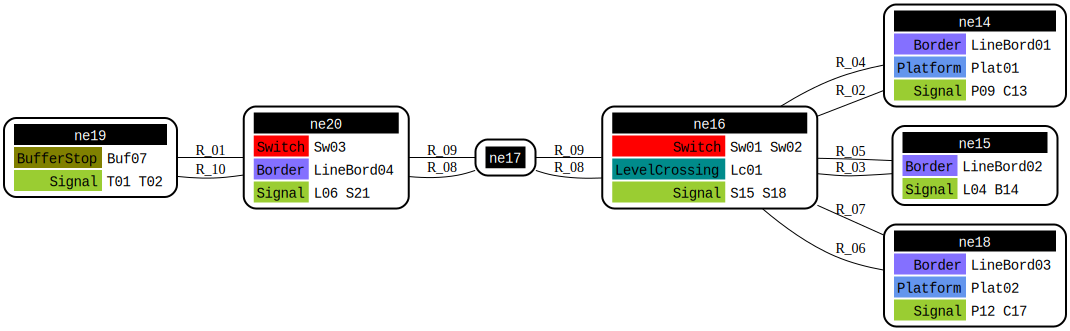
\includegraphics[width=1\textwidth]{Figuras/Graph_2}
    	\centering\caption{XXXX}
    	%\label{fig:LC_P2}
    \end{figure}
    
    \lipsum[1]

    \begin{figure}[h]
        \centering
        \includegraphics[width=1\textwidth]{resultados-obtenidos/ejemplo2/images/2_original.png}
        \centering\caption{Señalamiento original del ejemplo 2.}
        %\label{fig:LC_P2}
    \end{figure}

    \begin{figure}[h]
        \centering
        \includegraphics[width=1\textwidth]{resultados-obtenidos/ejemplo2/images/2_empty.png}
        \centering\caption{Topología ferroviaria del ejemplo 2 sin señalamiento.}
        %\label{fig:LC_P2}
    \end{figure}

    \begin{figure}[h]
        \centering
        \includegraphics[width=1\textwidth]{resultados-obtenidos/ejemplo2/images/2_step1.png}
        \centering\caption{Señalamiento generado por el RNA para proteger el fín de vía.}
        %\label{fig:LC_P2}
    \end{figure}

    \begin{figure}[h]
        \centering
        \includegraphics[width=1\textwidth]{resultados-obtenidos/ejemplo2/images/2_step2.png}
        \centering\caption{Señalamiento generado por el RNA para proteger las junturas.}
        %\label{fig:LC_P2}
    \end{figure}

    \begin{figure}[h]
        \centering
        \includegraphics[width=1\textwidth]{resultados-obtenidos/ejemplo2/images/2_step3.png}
        \centering\caption{Señalamiento generado por el RNA para proteger plataformas y cruces de vía.}
        %\label{fig:LC_P2}
    \end{figure}

    \begin{figure}[h]
        \centering
        \includegraphics[width=1\textwidth]{resultados-obtenidos/ejemplo2/images/2_step4.png}
        \centering\caption{Señalamiento generado por el RNA para proteger las máquinas de cambios.}
        %\label{fig:LC_P2}
    \end{figure}

    \begin{figure}[h]
        \centering
        \includegraphics[width=1\textwidth]{resultados-obtenidos/ejemplo2/images/2_RNA.png}
        \centering\caption{Señalamiento generado y simplificado por el RNA.}
        %\label{fig:LC_P2}
    \end{figure}
    
    \subsection{Señalamiento original}

    \lipsum[1]
    
    \begin{table}[!h]
        {
        \caption{Tabla de enclavamiento original del ejemplo 2.}
        \label{Tab:tabla_original_2}
        \centering
        \resizebox{1\textwidth}{!}{
            \begin{tabular}{ c c c c c c c }
                \hline	
                    Ruta & Inicio & Final & Cambio & Plataforma & Cruce & netElement \\	
                \hline
                    R$_{01}$  & S$_{07}$ & S$_{11}$ & Sw$_{01}^{N}$ & - & - & ne$_{14}$-ne$_{16}$\\
                    R$_{02}$  & S$_{08}$ & S$_{11}$ & Sw$_{01}^{R}$ & - & - & ne$_{15}$-ne$_{16}$\\
                    R$_{03}$  & S$_{09}$ & S$_{12}$ & Sw$_{02}^{N}$ & - & - & ne$_{18}$-ne$_{16}$\\
                    R$_{04}$  & S$_{10}$ & S$_{13}$ & Sw$_{03}^{N}$ & - & - & ne$_{20}$-ne$_{19}$\\
                    R$_{05}$  & S$_{10}$ & S$_{12}$ & Sw$_{03}^{R}$+Sw$_{02}^{R}$ & - & - & ne$_{20}$-ne$_{17}$-ne$_{16}$\\  
                \hline
            \end{tabular}
        }
     }
    \end{table}
    \subsection{Señalamiento generado por el RNA}

    \lipsum[1]
    
    \begin{table}[!h]
        {
        \caption{Tabla de enclavamiento del ejemplo 2 generada por el RNA.}
        \label{Tab:tabla_generated_2}
        \centering
        \resizebox{1\textwidth}{!}{
            \begin{tabular}{ c c c c c c c }
                \hline	
                    Ruta & Inicio & Final & Cambio & Plataforma & Cruce & netElement \\	
                \hline
                    R$_{01}$  & T$_{02}$ & L$_{06}$ & Sw$_{03}^{N}$ & - & - & ne$_{19}$-ne$_{20}$\\
                    R$_{02}$  & C$_{13}$ & S$_{18}$ & Sw$_{01}^{N}$ & - & - & ne$_{14}$-ne$_{16}$\\
                    R$_{03}$  & B$_{14}$ & S$_{18}$ & Sw$_{01}^{R}$ & - & - & ne$_{15}$-ne$_{16}$\\
                    R$_{04}$  & S$_{15}$ & P$_{09}$ & Sw$_{01}^{N}$ & Plat$_{01}$ & Lc$_{01}$ & ne$_{16}$-ne$_{14}$\\
                    R$_{05}$  & S$_{15}$ & L$_{04}$ & Sw$_{01}^{R}$ & Plat$_{01}$ & Lc$_{01}$ & ne$_{16}$-ne$_{15}$\\
                    R$_{06}$  & C$_{17}$ & S$_{15}$ & Sw$_{02}^{N}$ & - & - & ne$_{18}$-ne$_{16}$\\
                    R$_{07}$  & S$_{18}$ & P$_{12}$ & Sw$_{02}^{N}$ & Plat$_{02}$ & Lc$_{01}$ & ne$_{16}$-ne$_{18}$\\
                    R$_{08}$  & S$_{18}$ & L$_{06}$ & Sw$_{02}^{R}$+Sw$_{03}^{R}$ & - & Lc$_{01}$ & ne$_{16}$-ne$_{20}$\\
                    R$_{09}$  & S$_{21}$ & S$_{15}$ & Sw$_{02}^{R}$+Sw$_{03}^{R}$ & - & - & ne$_{20}$-ne$_{16}$\\
                    R$_{10}$  & S$_{21}$ & T$_{01}$ & Sw$_{03}^{N}$ & - & - & ne$_{20}$-ne$_{19}$\\
                \hline
            \end{tabular}
        }
     }
    \end{table}
    \subsection{Sistema generado por el ACG}

\lipsum[1]
\lipsum[1]
\lipsum[1]
    \section{Validación del sistema de enclavamientos}

	La validación de las rutas de la tabla de enclavamientos es realizada por el RNA aplicando el Algoritmo \ref{alg:interlocking_tables}, explicado en la Sección \ref{sec:validar_tabla}. Las 5 rutas del señalamiento original (Tabla \ref{Tab:tabla_original_2}) tienen 5 rutas equivalentes en el señalamiento generado por el RNA (Tabla \ref{Tab:tabla_generated_2}), tal como se puede visualizar en la Tabla \ref{Tab:tabla_validation_2}, generada automáticamente por el RNA.

    \begin{table}[H]
        {
        \caption{Equivalencias entre las rutas originales y las generadas por el RNA.}
        \label{Tab:tabla_validation_2}
        \centering
        %\small
            %\centering
            \begin{center}
            \resizebox{0.7\textwidth}{!}{
            \begin{tabular}{ c c c c }
                \hline	
                    Original & Señales & RNA & Señales \\	
                \hline
                    R$_{01}$ & S$_{07}$-S$_{11}$ & R$_{03}$ & B$_{14}$-S$_{18}$ \\
                    R$_{02}$ & S$_{08}$-S$_{11}$ & R$_{06}$ & C$_{17}$-S$_{15}$ \\
                    R$_{03}$ & S$_{09}$-S$_{12}$ & R$_{02}$ & C$_{13}$-S$_{18}$ \\
                    R$_{04}$ & S$_{10}$-S$_{13}$ & R$_{10}$ & S$_{21}$-S$_{15}$ \\
                    R$_{05}$ & S$_{10}$-S$_{12}$ & R$_{09}$ & S$_{21}$-S$_{15}$ \\
                \hline
            \end{tabular}
            }
            \end{center}
        }    
    \end{table}
        
    El RNA generó nuevas rutas para incrementar la seguridad de la red. La ruta R1 fue definida al crear las señales T02 y L06 para proteger el final de la vía en la sección ne19-ne20. La ruta R6 fue definida al crear la señal L04 para proteger el final de la vía en ne15, creando una nueva ruta con la señal S15. La ruta R8 fue definida al crear la señal L06 para proteger el final de la vía ne20, creando una nueva ruta con la señal S18.
    
    Adicionalmente, el RNA generó nuevas rutas para incrementar la movilidad de la red. La ruta R5 fue definida al crear la señal de partida P09 para la plataforma plat01. La ruta R7 fue definida al crear la señal de partida P12 para la plataforma plat02.
    
    Estos elementos ferroviarios, los finales de vía y las plataformas, no se encontraban protegidos en la tabla de enclavamientos original (Tabla \ref{Tab:tabla_original_2}). Ninguna ruta original atravesaba el cruce de vías, por lo que el RNA agregó las rutas R5 y R8 que cumplen esa función.
    
    Para finalizar, el RNA comprueba los principios de señalamiento ferroviario explicados en la Sección \label{sec:validar_principios}, aplicando los algoritmos indicados, de los cuáles se obtuvieron los siguientes resultados:
    
    \begin{itemize}
    	\item Principio de autoridad (Algoritmo \ref{alg:ppio_autoridad}): cobertura del 100\% de los \textit{netElements}.
    	\item Principio de claridad (Algoritmo \ref{alg:ppio_claridad}): rutas 100\% independientes.
    	\item Principio de anticipación (Algoritmo \ref{alg:ppio_anticipacion}): cobertura del 100\% de los puntos críticos.
    	\item Principio de granularidad (Algoritmo \ref{alg:ppio_granularidad}): 100\% de rutas divididas a su mínima expresión.
    	\item Principio de terminalidad (Algoritmo \ref{alg:ppio_terminalidad}): 100\% de finales de vías protegidos.
    	\item Principio de infraestructura (Algoritmo \ref{alg:ppio_infraestructura}): 100\% de infraestructura protegida.
    	\item Principio de no bloqueo (Algoritmo \ref{alg:ppio_nobloqueo}): 100\% de cambios de vías protegidos.
    \end{itemize}	
	%\section{Ejemplo 3}

    \lipsum[1]

    \begin{figure}[h]
        \centering
        \includegraphics[width=1\textwidth]{resultados-obtenidos/ejemplo3/images/3_original.png}
        \centering\caption{Señalamiento original del ejemplo 3.}
        %\label{fig:LC_P2}
    \end{figure}

    \begin{figure}[h]
        \centering
        \includegraphics[width=1\textwidth]{resultados-obtenidos/ejemplo3/images/3_empty.png}
        \centering\caption{Topología ferroviaria del ejemplo 3 sin señalamiento.}
        %\label{fig:LC_P2}
    \end{figure}

    \begin{figure}[h]
        \centering
        \includegraphics[width=1\textwidth]{resultados-obtenidos/ejemplo3/images/3_step1.png}
        \centering\caption{Señalamiento generado por el RNA para proteger el fín de vía.}
        %\label{fig:LC_P2}
    \end{figure}

    \begin{figure}[h]
        \centering
        \includegraphics[width=1\textwidth]{resultados-obtenidos/ejemplo3/images/3_step2.png}
        \centering\caption{Señalamiento generado por el RNA para proteger las junturas.}
        %\label{fig:LC_P2}
    \end{figure}

    \begin{figure}[h]
        \centering
        \includegraphics[width=1\textwidth]{resultados-obtenidos/ejemplo3/images/3_step3.png}
        \centering\caption{Señalamiento generado por el RNA para proteger plataformas y cruces de vía.}
        %\label{fig:LC_P2}
    \end{figure}

    \begin{figure}[h]
        \centering
        \includegraphics[width=1\textwidth]{resultados-obtenidos/ejemplo3/images/3_step4.png}
        \centering\caption{Señalamiento generado por el RNA para proteger las máquinas de cambios.}
        %\label{fig:LC_P2}
    \end{figure}

    \begin{figure}[h]
        \centering
        \includegraphics[width=1\textwidth]{resultados-obtenidos/ejemplo3/images/3_RNA.png}
        \centering\caption{Señalamiento generado y simplificado por el RNA.}
        %\label{fig:LC_P2}
    \end{figure}

    \subsection{Señalamiento original}

    \lipsum[1]
    
    \begin{table}[H]
        {
        \caption{Tabla de enclavamiento original del ejemplo 3.}
        \label{Tab:tabla_original_3}
        \centering
        \resizebox{1\textwidth}{!}{
            \begin{tabular}{ c c c c c c c }
                \hline	
                    Ruta & Inicio & Final & Cambio & Plataforma & Cruce & netElement \\	
                \hline
                    R$_{01}$ & 68N1 & 69Va & - & - & Lc$_{01}$ & ne$_{7}$-ne$_{95}$\\
                    R$_{02}$ & 68N2 & 69Va & - & - & Lc$_{01}$ & ne$_{1}$-ne$_{95}$\\
                    R$_{03}$ & 69Va & 69A & - & - & - & ne$_{95}$-ne$_{59}$\\
                    R$_{04}$ & 69A & 69N2 & 69W$_{03}^{N}$ & Plat$_{09}$ & - & ne$_{59}$-ne$_{17}$\\
                    R$_{05}$ & 69A & 69N3 & 69W$_{03}^{R}$ & Plat$_{13}$ & - & ne$_{59}$-ne$_{77}$\\
                    R$_{06}$ & 69P2 & 68F & - & - & - & ne$_{17}$-ne$_{9}$\\
                    R$_{07}$ & 69B2 & 69P2 & Sw$_{06}^{N}$ & Plat$_{09}$ & - & ne$_{78}$-ne$_{17}$\\
                    R$_{08}$ & 69B2 & 69P3 & Sw$_{06}^{R}$+Sw$_{07}^{S}$ & Plat$_{13}$ & - & ne$_{78}$-ne$_{77}$\\
                    R$_{09}$ & 69B2 & 69P1 & Sw$_{06}^{R}$+Sw$_{07}^{T}$ & Plat$_{12}$ & - & ne$_{78}$-ne$_{21}$\\
                    R$_{10}$ & 69C & 69N1 & - & Plat$_{12}$ & - & ne$_{70}$-ne$_{21}$\\
                    R$_{11}$ & 69Vc1 & 69C & - & - & -  & ne$_{70}$-ne$_{70}$\\
                    R$_{12}$ & 69Vc & 69Vc1 & - & Plat$_{07}$ & - & ne$_{67}$-ne$_{70}$\\
                    R$_{13}$ & 70Va & 70A & - & - & -  & ne$_{103}$-ne$_{64}$\\
                    R$_{14}$ & 70N2 & 69Vc & - & - & -  & ne$_{23}$-ne$_{67}$\\
                    R$_{15}$ & 70N1 & 69Vc & - & - & - & ne$_{24}$-ne$_{67}$\\
                    R$_{16}$ & 70P1 & 72Va & - & - & - & ne$_{24}$-ne$_{44}$\\
                    R$_{17}$ & 70P2 & 72Va & - & - & - & ne$_{23}$-ne$_{44}$\\
                    R$_{18}$ & 70B & 70N2 & 70W$_{02}^{N}$ & Plat$_{05}$ & - & ne$_{26}$-ne$_{23}$\\
                    R$_{19}$ & 70B & 70N1 & 70W$_{02}^{R}$ & Plat$_{06}$ & - & ne$_{26}$-ne$_{24}$\\
                    R$_{20}$ & 70A & 70P1 & 70W$_{01}^{N}$ & Plat$_{06}$ & - & ne$_{64}$-ne$_{24}$\\
                    R$_{21}$ & 70A & 70P2 & 70W$_{01}^{R}$ & Plat$_{05}$ & - & ne$_{64}$-ne$_{23}$\\
                    R$_{22}$ & 69W04Y & 69N3 & - & Plat$_{13}$ & - & ne$_{14}$-ne$_{77}$\\
                    R$_{23}$ & 72Va & 72A & - & - & - & ne$_{44}$-ne$_{100}$\\
                    R$_{24}$ & 721 & S01 & - & - & - & ne$_{83}$-ne$_{32}$\\
                    R$_{25}$ & 723b & S01 & Sw$_{05}^{T}$ & - & - & ne$_{41}$-ne$_{32}$\\
                    R$_{26}$ & 723b & 72B & Sw$_{05}^{S}$ & - & - & ne$_{41}$-ne$_{100}$\\
                    R$_{27}$ & 722 & 72B & - & - & - & ne$_{29}$-ne$_{100}$\\
                    R$_{28}$ & S01 & 72B & - & - & - & ne$_{32}$-ne$_{100}$\\
                    R$_{29}$ & 69B1 & 69P3 & Sw$_{07}^{T}$ & Plat$_{13}$ & - & ne$_{94}$-ne$_{77}$\\
                    R$_{30}$ & 69B1 & 69P1 & Sw$_{07}^{S}$ & Plat$_{12}$ & - & ne$_{94}$-ne$_{21}$\\
                    R$_{31}$ & 72B & 70B & 71W$_{01}^{N}$ & - & - & ne$_{100}$-ne$_{26}$\\
                    R$_{32}$ & 69P3 & 68F & 69W$_{04}^{R}$ & - & - & ne$_{77}$-ne$_{9}$\\
                    R$_{33}$ & 69P1 & 70Va & - & - & - & ne$_{21}$-ne$_{103}$\\
                \hline
            \end{tabular}
        }
     }
    \end{table}
    
    \lipsum[1]
    \subsection{Señalamiento generado por el RNA}

    El RNA también exporta la misma información mostrada en el Código \ref{lst:EJ3_8} en una hoja de cálculo. Por una cuestión de extensión, se particionará la tabla de enclavamientos en seis tablas. Las rutas 1 a 15 se visualizan en la Tabla \ref{Tab:tabla_generated_3_1}.
    
    \begin{table}[H]
        {
        \caption{Tabla de enclavamiento del ejemplo 3 generada por el RNA (Rutas 1 a 15).}
        \label{Tab:tabla_generated_3_1}
        \centering
        \resizebox{1\textwidth}{!}{
            \begin{tabular}{ c c c c c c c }
                \hline	
                    Ruta & Inicio & Final & Cambio & Plataforma & Cruce & netElement\\	
                \hline
                    R$_{01}$ & T$_{02}$ & C$_{78}$ & - & Plat$_{01}$ & - & ne$_{1}$-ne$_{1}$\\
                    R$_{02}$ & T$_{06}$ & J$_{43}$ & - & Plat$_{02}$ & - & ne$_{7}$-ne$_{7}$\\
                    R$_{03}$ & T$_{08}$ & P$_{146}$ & 69W$_{04}^{N}$ & - & - & ne$_{14}$-ne$_{52}$\\
                    R$_{04}$ & T$_{12}$ & L$_{29}$ & 71W$_{02}^{R}$ & - & - & ne$_{47}$-ne$_{48}$\\
                    R$_{05}$ & T$_{14}$ & C$_{100}$ & Sw$_{04}^{R}$ & - & - & ne$_{84}$-ne$_{32}$\\
                    R$_{06}$ & T$_{14}$ & S$_{105}$ & Sw$_{41}^{R}$ & - & - & ne$_{84}$-ne$_{44}$\\
                    R$_{07}$ & T$_{20}$ & S$_{97}$ & Sw$_{12}^{N}$ & - & - & ne$_{89}$-ne$_{30}$\\
                    R$_{08}$ & T$_{22}$ & S$_{97}$ & Sw$_{12}^{R}$+Sw$_{13}^{R}$ & - & - & ne$_{90}$-ne$_{30}$\\
                    R$_{09}$ & T$_{24}$ & P$_{70}$ & - & Plat$_{11}$ & - & ne$_{105}$-ne$_{96}$\\
                    R$_{10}$ & L$_{25}$ & L$_{42}$ & - & - & - & ne$_{4}$-ne$_{106}$\\
                    R$_{11}$ & L$_{27}$ & L$_{30}$ & - & - & - & ne$_{26}$-ne$_{65}$\\
                    R$_{12}$ & L$_{28}$ & L$_{40}$ & - & - & - & ne$_{44}$-ne$_{101}$\\
                    R$_{13}$ & L$_{30}$ & C$_{104}$ & - & - & - & ne$_{65}$-ne$_{102}$\\
  					R$_{14}$ & L$_{32}$ & P$_{73}$ & Sw$_{03}^{N}$ & - & - & ne$_{70}$-ne$_{21}$\\
  					R$_{15}$ & L$_{33}$ & L$_{34}$ & - & - & - & ne$_{78}$-ne$_{93}$\\
                \hline
            \end{tabular}
        }
     }
    \end{table}

	Las rutas 16 a 30 se visualizan en la Tabla \ref{Tab:tabla_generated_3_2}.
	
    \begin{table}[H]
        {
        \caption{Tabla de enclavamiento del ejemplo 3 generada por el RNA (Rutas 16 a 30).}
        \label{Tab:tabla_generated_3_2}
        \centering
        \resizebox{1\textwidth}{!}{
            \begin{tabular}{ c c c c c c c }
                \hline	
                    Ruta & Inicio & Final & Cambio & Plataforma & Cruce & netElement\\	
                \hline
                    R$_{16}$ & L$_{34}$ & P$_{71}$ & - & Plat$_{11}$ & - & ne$_{93}$-ne$_{96}$\\
                    R$_{17}$ & L$_{35}$ & X$_{50}$ & - & - & - & ne$_{95}$-ne$_{95}$\\
                    R$_{18}$ & L$_{37}$ & S$_{135}$ & - & - & - & ne$_{97}$-ne$_{94}$\\
                    R$_{19}$ & L$_{38}$ & T$_{23}$ & - & - & - & ne$_{98}$-ne$_{105}$\\
                    R$_{20}$ & L$_{40}$ & S$_{139}$ & - & - & - & ne$_{101}$-ne$_{100}$\\
                    R$_{21}$ & L$_{41}$ & S$_{90}$ & - & - & - & ne$_{103}$-ne$_{64}$\\
                    R$_{22}$ & L$_{42}$ & P$_{68}$ & - & Plat$_{10}$ & - & ne$_{106}$-ne$_{99}$\\
                    R$_{23}$ & J$_{43}$ & J$_{46}$ & 68W$_{02}^{R}$ & - & - & ne$_{7}$-ne$_{9}$\\
                    R$_{24}$ & J$_{46}$ & L$_{35}$ & - & - & - & ne$_{9}$-ne$_{95}$\\
                    R$_{25}$ & X$_{50}$ & S$_{83}$ & - & - & Lc01 & ne$_{95}$-ne$_{59}$\\
                    R$_{26}$ & X$_{51}$ & S$_{80}$ & - & - & Lc01 & ne$_{95}$-ne$_{9}$\\
                    R$_{27}$ & P$_{60}$ & L$_{27}$ & 70W$_{02}^{N}$ & - & - & ne$_{23}$-ne$_{26}$\\
                    R$_{28}$ & P$_{63}$ & L$_{41}$ & 70W$_{01}^{N}$ & - & - & ne$_{24}$-ne$_{103}$\\
                    R$_{29}$ & P$_{64}$ & L$_{32}$ & - & - & - & ne$_{67}$-ne$_{70}$\\
                    R$_{30}$ & P$_{65}$ & L$_{41}$ & - & - & - & ne$_{67}$-ne$_{103}$\\
                \hline
            \end{tabular}
        }
     }
    \end{table}

	Las rutas 31 a 45 se visualizan en la Tabla \ref{Tab:tabla_generated_3_3}.
	
    \begin{table}[H]
        {
        \caption{Tabla de enclavamiento del ejemplo 3 generada por el RNA (Rutas 31 a 45).}
        \label{Tab:tabla_generated_3_3}
        \centering
        \resizebox{1\textwidth}{!}{
            \begin{tabular}{ c c c c c c c }
                \hline	
                    Ruta & Inicio & Final & Cambio & Plataforma & Cruce & netElement\\	
                \hline     
                    R$_{31}$ & P$_{68}$ & L$_{37}$ & - & - & - & ne$_{99}$-ne$_{97}$\\
                    R$_{32}$ & P$_{69}$ & T$_{03}$ & - & - & - & ne$_{99}$-ne$_{4}$\\
                    R$_{33}$ & P$_{70}$ & S$_{110}$ & - & - & - & ne$_{96}$-ne$_{78}$\\
                    R$_{34}$ & P$_{71}$ & L$_{38}$ & - & - & - & ne$_{96}$-ne$_{98}$\\
                    R$_{35}$ & P$_{72}$ & S$_{144}$ & - & - & - & ne$_{21}$-ne$_{21}$\\
                    R$_{36}$ & P$_{73}$ & L$_{33}$ & Sw$_{06}^{R}$ & - & - & ne$_{21}$-ne$_{78}$\\ 
                    R$_{37}$ & P$_{73}$ & P$_{69}$ & - & Plat$_{10}$ & - & ne$_{21}$-ne$_{99}$\\
                    R$_{38}$ & C$_{78}$ & J$_{46}$ & 68W$_{02}^{N}$ & - & - & ne$_{1}$-ne$_{9}$\\
                    R$_{39}$ & S$_{80}$ & T$_{01}$ & 68W$_{02}^{N}$ & Plat$_{01}$ & - & ne$_{9}$-ne$_{1}$\\
                    R$_{40}$ & S$_{80}$ & T$_{05}$ & 68W$_{02}^{R}$ & Plat$_{02}$ & - & ne$_{9}$-ne$_{7}$\\
                    R$_{41}$ & S$_{82}$ & X$_{51}$ & 69W$_{03}^{N}$ & - & - & ne$_{17}$-ne$_{95}$\\
                    R$_{42}$ & S$_{83}$ & S$_{146}$ & 69W$_{03}^{R}$+69W$_{04}^{R}$ & - & - & ne$_{59}$-ne$_{52}$\\
                    R$_{43}$ & S$_{83}$ & S$_{109}$ & 69W$_{03}^{N}$ & Plat$_{09}$ & - & ne$_{59}$-ne$_{17}$\\
                    R$_{44}$ & S$_{86}$ & X$_{51}$ & 69W$_{03}^{R}$+69W$_{04}^{R}$ & - & - & ne$_{52}$-ne$_{95}$\\
                    R$_{45}$ & S$_{86}$ & T$_{07}$ & 69W$_{04}^{N}$ & - & - & ne$_{52}$-ne$_{14}$\\
                \hline
            \end{tabular}
        }
     }
    \end{table}

	Las rutas 46 a 60 se visualizan en la Tabla \ref{Tab:tabla_generated_3_4}.
	
    \begin{table}[H]
        {
        \caption{Tabla de enclavamiento del ejemplo 3 generada por el RNA (Rutas 46 a 60).}
        \label{Tab:tabla_generated_3_4}
        \centering
        \resizebox{1\textwidth}{!}{
            \begin{tabular}{ c c c c c c c }
                \hline	
                    Ruta & Inicio & Final & Cambio & Plataforma & Cruce & netElement\\	
                \hline
                    R$_{46}$ & B$_{89}$ & L$_{41}$ & 70W$_{01}^{R}$ & Plat$_{05}$ & - & ne$_{23}$-ne$_{103}$\\
                    R$_{47}$ & S$_{90}$ & P$_{60}$ & 70W$_{01}^{R}$ & Plat$_{05}$ & - & ne$_{64}$-ne$_{23}$\\
                    R$_{48}$ & S$_{90}$ & L$_{27}$ & 70W$_{01}^{R}$+70W$_{02}^{N}$ & Plat$_{05}$ & - & ne$_{64}$-ne$_{26}$\\
                    R$_{49}$ & B$_{92}$ & P$_{63}$ & - & - & - & ne$_{24}$-ne$_{24}$\\
                    R$_{50}$ & S$_{93}$ & B$_{89}$ & 70W$_{02}^{N}$ & - & - & ne$_{26}$-ne$_{23}$\\
                    R$_{51}$ & S$_{93}$ & P$_{92}$ & 70W$_{02}^{R}$ & Plat$_{06}$ & - & ne$_{26}$-ne$_{24}$\\
                    R$_{52}$ & S$_{95}$ & S$_{122}$ & Sw$_{08}^{N}$ & - & - & ne$_{83}$-ne$_{30}$\\
                    R$_{53}$ & S$_{96}$ & S$_{122}$ & Sw$_{08}^{R}$ & - & - & ne$_{29}$-ne$_{30}$\\
                    R$_{54}$ & S$_{97}$ & C$_{138}$ & Sw$_{08}^{R}$+Sw$_{09}^{R}$ & - & - & ne$_{30}$-ne$_{110}$\\
                    R$_{55}$ & S$_{97}$ & C$_{114}$ & Sw$_{08}^{N}$ & Plat$_{03}$ & - & ne$_{30}$-ne$_{83}$\\
                    R$_{56}$ & C$_{100}$ & S$_{138}$ & Sw$_{09}^{N}$ & - & - & ne$_{32}$-ne$_{110}$\\
                    R$_{57}$ & B$_{101}$ & S$_{96}$ & - & - & - & ne$_{29}$-ne$_{29}$\\
                    R$_{58}$ & S$_{102}$ & S$_{115}$ & Sw$_{09}^{N}$ & - & - & ne$_{110}$-ne$_{32}$\\
                    R$_{59}$ & S$_{102}$ & B$_{101}$ & Sw$_{09}^{R}$ & - & - & ne$_{110}$-ne$_{29}$\\
                    R$_{60}$ & C$_{104}$ & L$_{28}$ & 71W$_{01}^{N}$ & - & - & ne$_{102}$-ne$_{44}$\\
                \hline
            \end{tabular}
        }
     }
    \end{table}
    
    Las rutas 61 a 75 se visualizan en la Tabla \ref{Tab:tabla_generated_3_5}.
    
    \begin{table}[H]
        {
        \caption{Tabla de enclavamiento del ejemplo 3 generada por el RNA (Rutas 61 a 75).}
        \label{Tab:tabla_generated_3_5}
        \centering
        \resizebox{1\textwidth}{!}{
            \begin{tabular}{ c c c c c c c }
                \hline	
                    Ruta & Inicio & Final & Cambio & Plataforma & Cruce & netElement\\	
                \hline
                    R$_{61}$ & S$_{105}$ & L$_{29}$ & 71W$_{01}^{R}$+71W$_{02}^{N}$ & - & - & ne$_{44}$-ne$_{48}$\\
                    R$_{62}$ & S$_{105}$ & S$_{93}$ & 71W$_{01}^{N}$ & - & - & ne$_{44}$-ne$_{26}$\\
                    R$_{63}$ & C$_{109}$ & L$_{33}$ & Sw$_{06}^{N}$ & - & - & ne$_{17}$-ne$_{78}$\\
                    R$_{64}$ & S$_{110}$ & S$_{82}$ & Sw$_{06}^{N}$ & Plat$_{09}$ & - & ne$_{78}$-ne$_{17}$\\
                    R$_{65}$ & S$_{110}$ & B$_{133}$ & Sw$_{06}^{R}$+Sw$_{07}^{RR}$ & Plat$_{08}$+Plat$_{13}$ & - & ne$_{78}$-ne$_{77}$\\
                    R$_{66}$ & S$_{110}$ & P$_{72}$ & Sw$_{06}^{R}$+Sw$_{07}^{RN}$ & Plat$_{12}$ & - & ne$_{78}$-ne$_{21}$\\
                    R$_{67}$ & C$_{114}$ & C$_{100}$ & Sw$_{04}^{N}$ & - & - & ne$_{83}$-ne$_{32}$\\
                    R$_{68}$ & S$_{115}$ & C$_{95}$ & Sw$_{04}^{N}$ & Plat$_{03}$ & - & ne$_{32}$-ne$_{83}$\\
                    R$_{69}$ & S$_{115}$ & P$_{58}$ & Sw$_{04}^{R}$ & Plat$_{04}$ & - & ne$_{32}$-ne$_{41}$\\
                    R$_{70}$ & S$_{113}$ & T$_{13}$ & Sw$_{04}^{R}$ & - & - & ne$_{32}$-ne$_{84}$\\
                    R$_{71}$ & S$_{118}$ & T$_{15}$ & Sw$_{11}^{N}$ & - & - & ne$_{88}$-ne$_{86}$\\
                    R$_{72}$ & S$_{119}$ & T$_{17}$ & Sw$_{11}^{N}$ & - & - & ne$_{86}$-ne$_{88}$\\
                    R$_{73}$ & S$_{119}$ & S$_{97}$ & Sw$_{11}^{R}$+Sw$_{12}^{R}$+Sw$_{13}^{N}$ & - & - & ne$_{86}$-ne$_{30}$\\
                    R$_{74}$ & S$_{122}$ & T$_{19}$ & Sw$_{12}^{N}$ & - & - & ne$_{30}$-ne$_{89}$\\
                    R$_{75}$ & S1$_{22}$ & T$_{15}$ & Sw$_{11}^{R}$+Sw$_{12}^{R}$+Sw$_{13}^{N}$ & - & - & ne$_{30}$-ne$_{86}$\\
                \hline
            \end{tabular}
        }
     }
    \end{table}
    
    Las rutas 75 a 91 se visualizan en la Tabla \ref{Tab:tabla_generated_3_6}.
    
    \begin{table}[H]
        {
        \caption{Tabla de enclavamiento del ejemplo 3 generada por el RNA (Rutas 75 a 91).}
        \label{Tab:tabla_generated_3_6}
        \centering
        \resizebox{1\textwidth}{!}{
            \begin{tabular}{ c c c c c c c }
                \hline	
                    Ruta & Inicio & Final & Cambio & Plataforma & Cruce & netElement\\	
                \hline
                    R$_{76}$ & S$_{122}$ & T$_{21}$ & Sw$_{12}^{R}$+Sw$_{13}^{R}$ & - & - & ne$_{30}$-ne$_{90}$\\
                    R$_{77}$ & B$_{130}$ & C$_{100}$ & Sw$_{04}^{R}$+Sw$_{05}^{RN}$ & Plat$_{04}$ & - & ne$_{41}$-ne$_{32}$\\
                    R$_{78}$ & B$_{130}$ & S$_{105}$ & Sw$_{05}^{NN}$+Sw$_{41}^{R}$ & Plat$_{04}$ & - & ne$_{41}$-ne$_{44}$\\
                    R$_{79}$ & S$_{131}$ & P$_{58}$ & Sw$_{05}^{NN}$ & Plat$_{04}$ & - & ne$_{85}$-ne$_{41}$\\
                    R$_{80}$ & S$_{131}$ & T$_{13}$ & Sw$_{05}^{NR}$ & - & - & ne$_{85}$-ne$_{84}$\\
                    R$_{81}$ & B$_{133}$ & S$_{86}$ & - & - & - & ne$_{77}$-ne$_{52}$\\
                    R$_{82}$ & S$_{135}$ & B$_{133}$ & Sw$_{07}^{NR}$ & Plat$_{08}$+Plat$_{13}$ & - & ne$_{94}$-ne$_{77}$\\
                    R$_{83}$ & S$_{135}$ & P$_{72}$ & Sw$_{07}^{NN}$ & Plat$_{12}$ & - & ne$_{94}$-ne$_{21}$\\
                    R$_{84}$ & C$_{138}$ & S$_{105}$ & Sw$_{41}^{N}$ & - & - & ne$_{110}$-ne$_{44}$\\
                    R$_{85}$ & S$_{139}$ & S$_{102}$ & Sw$_{41}^{N}$ & - & - & ne$_{100}$-ne$_{110}$\\
                    R$_{86}$ & S$_{139}$ & S$_{131}$ & Sw$_{41}^{R}$ & - & - & ne$_{100}$-ne$_{85}$\\
                    R$_{87}$ & B$_{143}$ & L$_{32}$ & - & - & - & ne$_{104}$-ne$_{70}$\\
                    R$_{88}$ & S$_{144}$ & B$_{143}$ & - & - & - & ne$_{21}$-ne$_{104}$\\
                    R$_{89}$ & B$_{145}$ & L$_{33}$ & Sw$_{06}^{R}$+Sw$_{07}^{RR}$ & - & - & ne$_{77}$-ne$_{78}$\\
                    R$_{90}$ & B$_{145}$ & P$_{69}$ & Sw$_{07}^{NR}$ & Plat$_{10}$ & - & ne$_{77}$-ne$_{99}$\\
                    R$_{91}$ & S$_{146}$ & B$_{145}$ & - & Plat$_{08}$+Plat$_{13}$ & - & ne$_{52}$-ne$_{77}$\\
                \hline
            \end{tabular}
        }
     }
    \end{table}
    
    En una primera inspección podemos ver que el nuevo señalamiento tiene 91 rutas, versus las 33 rutas del señalamiento original. Esto se debe a la gran cantidad de secciones de la red que no cuentan con señalamiento apropiado.
    \section{Sistema generado por el ACG}

	En base a la red de grafos, ilustrada en la Figura \ref{fig:EJ3_8}, el ACG determinó la siguiente cantidad de elementos, tal puede visualizarse en el Código \ref{lst:EJ3_8}.
	
	\begin{lstlisting}[language = {}, caption = Cantidad de elementos a implementar por el ACG, label = {lst:EJ3_8}]
	n_netElements:53
	n_switch:15
	n_doubleSwitch:2
	n_borders:18
	n_buffers:12
	n_levelCrossings:1
	n_platforms:13
	n_scissorCrossings:1
	n_signals:82
	N : 245
	\end{lstlisting}
	
	Se repetirán los pasos detallados en el ejemplo 1, Sección \ref{sec:EJEMPLO1_ACG}, por lo que solamente se destacarán aspectos particulares de este ejemplo. El ACG genera 253 archivos en formato VHDL. El archivo \textit{Arty\_Z7-10.XDC} es el mismo para todos los ejemplos, al ser invariante respecto a la cantidad de pines a utilizar. Se deberá modificar el script mostrado en el Código \ref{lst:EJ1_script} y cambiar el parámetro \textit{chosen} a 3 para automatizar la importación de los archivos del ejemplo 3 y desvincular cualquier otro conjunto de archivos de ejemplos anteriores.
	
	Una vez ejecutado el script, Vivado ordenará los archivos de forma jerárquica, donde el módulo \textit{global} incluye todos los módulos que fueron detallados en la Sección \ref{sec:interlockingArch}. Cada una de las instancias del módulo \textit{network} contienen sus propias 245 instancias de los mismos módulos de cada elemento ferroviario ya que N, cantidad de elementos ferroviarios, es 245 en el Código \ref{lst:EJ3_8}. El ejemplo 3 utiliza mas de 70600 sub módulos conectados automáticamente mediante mas de 147300 señales, lo cual se aleja bastante de un desarrollo que pueda realizarse manualmente de forma trivial.
	
	Cuando Vivado genera el diagrama de bloques ya tenemos la certeza de que el código VHDL ha pasado la prueba de sintaxis del entorno de desarrollo. A continuación, se deberá sintetizar e implementar el sistema para generar el bitstream que será utilizado para programar la FPGA. Los procesos de síntesis e implementación fueron detallados en el ejemplo 1, Sección \ref{sec:EJEMPLO1_ACG}.
	
	Los resultados de ambos procesos son detallados en la Tabla \ref{Tab:tabla_ACG_3}. Los porcentajes de uso son calculados por Vivado automáticamente, teniendo en cuenta que la plataforma Arty Z7 20 posee 53200 Look-Up-Tables (LUTs), 106400 Flip-Flops (FFs), 125 Pines de entrada y salida (IOs) y 32 Buffers (BUFGs), tal cómo se explicó en la Sección \ref{sec:AGG}. En este ejemplo, la cantidad de recursos utilizados es intermedia y el tiempo de síntesis e implementación es de 2 minutos con 6 segundos y 3 minuto con 39 segundos, respectivamente.

	\begin{table}[H]
		{
			\caption{Síntesis e implementación del ejemplo 3 generado por el ACG.}
			\label{Tab:tabla_ACG_3}
			\centering
			%\small
			%\centering
			\begin{center}
				\resizebox{0.65\textwidth}{!}{
					\begin{tabular}{ c c c c }
						\hline	
						Recursos & Síntesis & Implementación & Uso \\	
						\hline
						LUT & 13626 & 13509 & 25.61-25.39\%\\
						FF & 15110 & 15113 & 14.20\%\\
						IO & 15 & 15 & 12.00\%\\
						BUFG & 3 & 3 & 9.38\%\\
						\hline
					\end{tabular}
				}
			\end{center}
		}    
	\end{table}
    \subsection{Validacion del sistema}

\lipsum[1]

    \begin{table}[!h]
        {
        \caption{Equivalencias entre las rutas originales y las generadas por el RNA (Rutas 1 a 16).}
        \label{Tab:tabla_original_1}
        \centering
        %\small
            %\centering
            \begin{center}
            \resizebox{1\textwidth}{!}{
            \begin{tabular}{ c c c c }
                \hline	
                    Original & Señales & RNA & Señales \\	
                \hline
                    R$_{01}$ & 68N1-69Va & R$_{26}$+R$_{27}$ & S$_{43}$-S$_{35}$\\
                    R$_{02}$ & 68N2-69Va & R$_{44}$+R$_{27}$ & S$_{78}$-S$_{35}$\\
                    R$_{03}$ & 69Va-69A & R$_{28}$ & S$_{50}$-S$_{83}$\\
                    R$_{04}$ & 69A-69N2 & R$_{49}$ & S$_{83}$-S$_{109}$\\
                    R$_{05}$ & 69A-69N3 & R$_{48}$ & S$_{83}$-S$_{77}$\\
                    R$_{06}$ & 69P2-68F & R$_{47}$+R$_{29}$ & S$_{82}$-S$_{80}$\\
                    R$_{07}$ & 69B2-69P2 & R$_{70}$ & S$_{110}$-S$_{82}$\\
                    R$_{08}$ & 69B2-69P3 & R$_{71}$ & S$_{110}$-S$_{76}$\\
                    R$_{09}$ & 69B2-69P1 & R$_{72}$ & S$_{110}$-S$_{72}$\\
                    R$_{10}$ & 69C-69N1 & R$_{16}$ & S$_{32}$-S$_{73}$\\
                    R$_{11}$ & 69Vc1-69C & R$_{38}$ & S$_{72}$-S$_{32}$\\
                    R$_{12}$ & 69Vc-69Vc1 & R$_{32}$ & S$_{64}$-S$_{32}$\\
                    R$_{13}$ & 70Va-70A & R$_{24}$ & S$_{41}$-S$_{90}$\\
                    R$_{14}$ & 70N2-69Vc & R$_{30}$ & S$_{60}$-S$_{27}$\\
                    R$_{15}$ & 70N1-69Vc & R$_{31}$ & S$_{63}$-S$_{41}$\\
                    R$_{16}$ & 70P1-72Va & R$_{31}$+R$_{24}$+R$_{54}$+R$_{13}$+R$_{15}$+R$_{66}$ & S$_{63}$-S$_{28}$\\
                \hline
            \end{tabular}
            }
            \end{center}
        }    
    \end{table}

    \begin{table}[!h]
        {
        \caption{Equivalencias entre las rutas originales y las generadas por el RNA (Rutas 17 a 33).}
        \label{Tab:tabla_original_1}
        \centering
        %\small
            %\centering
            \begin{center}
            \resizebox{1\textwidth}{!}{
            \begin{tabular}{ c c c c }
                \hline	
                    Original & Señales & RNA & Señales \\	
                \hline
                    R$_{17}$ & 70P2-72Va & R$_{30}$+R$_{13}$+R$_{15}$+R$_{66}$ & S$_{60}$-S$_{28}$\\
                    R$_{18}$ & 70B-70N2 & R$_{56}$ & S$_{93}$-S$_{89}$\\
                    R$_{19}$ & 70B-70N1 & R$_{57}$ & S$_{93}$-S$_{92}$\\
                    R$_{20}$ & 70A-70P1 & R$_{54}$+R$_{57}$ & S$_{90}$-S$_{92}$\\
                    R$_{21}$ & 70A-70P2 & R$_{53}$ & S$_{90}$-S$_{60}$\\
                    R$_{22}$ & 69W04Y-69N3 & R$_{03}$ & S$_{08}$-S$_{77}$\\
                    R$_{23}$ & 72Va-72A & R$_{14}$+R$_{23}$ & S$_{28}$-S$_{126}$\\
                    R$_{24}$ & 721-S01 & R$_{73}$ & S$_{112}$-S$_{100}$\\
                    R$_{25}$ & 723b-S01 & R$_{04}$ & S$_{10}$-S$_{100}$\\
                    R$_{26}$ & 723b-72B & R$_{05}$+R$_{14}$+R$_{23}$ & S$_{10}$-S$_{126}$\\
                    R$_{27}$ & 722-72B & R$_{59}$+R$_{60}$+R$_{83}$+R$_{14}$+R$_{23}$ & S$_{96}$-S$_{126}$\\
                    R$_{28}$ & S01-72B & R$_{62}$+R$_{83}$+R$_{14}$+R$_{23}$ & S$_{100}$-S$_{126}$\\
                    R$_{29}$ & 69B1-69P3 & R$_{48}$ & S$_{83}$-S$_{77}$\\
                    R$_{30}$ & 69B1-69P1 & R$_{21}$ & S$_{37}$-S$_{72}$\\
                    R$_{31}$ & 72B-70B & R$_{86}$+R$_{83}$+R$_{68}$ & S$_{126}$-S$_{93}$\\
                    R$_{32}$ & 69P3-68F & R$_{41}$+R$_{50}$+R$_{29}$ & S$_{76}$-S$_{80}$\\
                    R$_{33}$ & 69P1-70Va & R$_{38}$ & S$_{72}$-S$_{32}$\\
                \hline
            \end{tabular}
            }
            \end{center}
        }    
    \end{table}
	%\section{Ejemplo 4}

    \lipsum[1]

    \begin{figure}[h]
        \centering
        \includegraphics[width=1\textwidth]{resultados-obtenidos/ejemplo4/images/4_original.png}
        \centering\caption{Señalamiento original del ejemplo 4.}
        %\label{fig:LC_P2}
    \end{figure}

    \lipsum[1]
    
    \begin{figure}[h]
        \centering
        \includegraphics[width=1\textwidth]{resultados-obtenidos/ejemplo4/images/4_empty.png}
        \centering\caption{Topología ferroviaria del ejemplo 4 sin señalamiento.}
        %\label{fig:LC_P2}
    \end{figure}

    \begin{figure}[h]
        \centering
        \includegraphics[width=1\textwidth]{resultados-obtenidos/ejemplo4/images/4_step1.png}
        \centering\caption{Señalamiento generado por el RNA para proteger el fín de vía.}
        %\label{fig:LC_P2}
    \end{figure}

    \begin{figure}[h]
        \centering
        \includegraphics[width=1\textwidth]{resultados-obtenidos/ejemplo4/images/4_step2.png}
        \centering\caption{Señalamiento generado por el RNA para proteger las junturas.}
        %\label{fig:LC_P2}
    \end{figure}

    \begin{figure}[h]
        \centering
        \includegraphics[width=1\textwidth]{resultados-obtenidos/ejemplo4/images/4_step3.png}
        \centering\caption{Señalamiento generado por el RNA para proteger plataformas y cruces de vía.}
        %\label{fig:LC_P2}
    \end{figure}

    \begin{figure}[h]
        \centering
        \includegraphics[width=1\textwidth]{resultados-obtenidos/ejemplo4/images/4_step4.png}
        \centering\caption{Señalamiento generado por el RNA para proteger las máquinas de cambios.}
        %\label{fig:LC_P2}
    \end{figure}

    \begin{figure}[h]
        \centering
        \includegraphics[width=1\textwidth]{resultados-obtenidos/ejemplo4/images/4_RNA.png}
        \centering\caption{Señalamiento generado y simplificado por el RNA.}
        %\label{fig:LC_P2}
    \end{figure}

    \subsection{Señalamiento original}

    \lipsum[1]
    
    \begin{table}[H]
        {
        \caption{Tabla de enclavamiento original del ejemplo 4 (Rutas 1 a 15).}
        \label{Tab:tabla_original_4_1}
        \centering
        \resizebox{1\textwidth}{!}{
            \begin{tabular}{ c c c c c c c }
                \hline	
                    Ruta & Inicio & Final & Cambio & Plataforma & Cruce & netElement \\	
                \hline
                    R$_{01}$ & S$_{15}$ & S$_{24}$ & - & - & Lc$_{02}$ & ne$_{98}$-ne$_{99}$\\
                    R$_{02}$ & S$_{16}$ & S$_{67}$ & Sw$_{04}^{N}$ & - & Lc$_{02}$ & ne$_{98}$-ne$_{292}$\\
                    R$_{03}$ & S$_{16}$ & S$_{43}$ & Sw$_{04}^{R}$ & - & Lc$_{02}$ & ne$_{98}$-ne$_{297}$\\
                    R$_{04}$ & S$_{19}$ & S$_{32}$ & - & - & Lc$_{06}$ & ne$_{100}$-ne$_{101}$\\
                    R$_{05}$ & S$_{20}$ & S$_{11}$ & Sw$_{01}^{N}$ & - & Lc$_{06}$ & ne$_{100}$-ne$_{65}$\\
                    R$_{06}$ & S$_{20}$ & S$_{56}$ & Sw$_{01}^{R}$ & - & Lc$_{06}$ & ne$_{100}$-ne$_{400}$\\
                    R$_{07}$ & S$_{23}$ & S$_{16}$ & - & - & - & ne$_{63}$-ne$_{98}$\\
                    R$_{08}$ & S$_{24}$ & S$_{80}$ & D$_{05}^{N}$ & - & - & ne$_{99}$-ne$_{63}$\\
                    R$_{09}$ & S$_{24}$ & S$_{52}$ & D$_{05}^{R}$-D$_{08}^{N}$ & - & - & ne$_{99}$-ne$_{404}$\\
                    R$_{10}$ & S$_{24}$ & S$_{57}$ & D$_{05}^{R}$-D$_{08}^{R}$ & - & - & ne$_{99}$-ne$_{123}$\\
                    R$_{11}$ & S$_{27}$ & S$_{56}$ & - & - & - & ne$_{993}$-ne$_{400}$\\
                    R$_{12}$ & S$_{28}$ & S$_{04}$ & Sw$_{02}^{N}$ & - & - & ne$_{400}$-ne$_{384}$\\
                    R$_{13}$ & S$_{28}$ & S$_{19}$ & Sw$_{02}^{R}$ & - & Lc$_{05}$ & ne$_{400}$-ne$_{100}$\\
                    R$_{14}$ & S$_{31}$ & S$_{20}$ & - & - & - & ne$_{912}$-ne$_{100}$\\
                    R$_{15}$ & S$_{32}$ & S$_{91}$ & D$_{09}^{N}$ & - & - & ne$_{101}$-ne$_{912}$\\    
                \hline
            \end{tabular}
        }
     }
    \end{table}

	\lipsum[1]
	
    \begin{table}[H]
        {
        \caption{Tabla de enclavamiento original del ejemplo 4 (Rutas 16 a 30).}
        \label{Tab:tabla_original_4_2}
        \centering
        \resizebox{1\textwidth}{!}{
            \begin{tabular}{ c c c c c c c }
                \hline	
                    Ruta & Inicio & Final & Cambio & Plataforma & Cruce & netElement \\	
                \hline
                    R$_{16}$ & S$_{32}$ & S$_{59}$ & D$_{09}^{R}$-D$_{10}^{N}$ & - & - & ne$_{101}$-ne$_{130}$\\
                    R$_{17}$ & S$_{32}$ & S$_{60}$ & D$_{09}^{R}$-D$_{10}^{R}$ & - & - & ne$_{101}$-ne$_{135}$\\
                    R$_{18}$ & S$_{35}$ & S$_{01}$ & - & - & - & ne$_{290}$-ne$_{130}$\\
                    R$_{19}$ & S$_{39}$ & S$_{43}$ & - & - & - & ne$_{995}$-ne$_{297}$\\
                    R$_{20}$ & S$_{44}$ & S$_{04}$ & - & - & - & ne$_{110}$-ne$_{384}$\\
                    R$_{21}$ & S$_{45}$ & S$_{01}$ & - & - & - & ne$_{295}$-ne$_{130}$\\
                    R$_{22}$ & S$_{46}$ & S$_{63}$ & Sw$_{02}^{N}$ & - & - & ne$_{384}$-ne$_{110}$\\
                    R$_{23}$ & S$_{46}$ & S$_{09}$ & Sw$_{02}^{R}$ & - & - & ne$_{384}$-ne$_{292}$\\
                    R$_{24}$ & S$_{47}$ & S$_{40}$ & - & - & - & ne$_{295}$-ne$_{297}$\\
                    R$_{25}$ & S$_{52}$ & S$_{28}$ & - & - & - & ne$_{404}$-ne$_{400}$\\
                    R$_{26}$ & S$_{56}$ & S$_{58}$ & D$_{07}^{N}$ & - & - & ne$_{400}$-ne$_{404}$\\
                    R$_{27}$ & S$_{56}$ & S$_{03}$ & D$_{07}^{R}$ & - & - & ne$_{400}$-ne$_{407}$\\
                    R$_{28}$ & S$_{57}$ & S$_{76}$ & - & - & - & ne$_{123}$-ne$_{407}$\\
                    R$_{29}$ & S$_{58}$ & S$_{16}$ & - & - & - & ne$_{404}$-ne$_{98}$\\
                    R$_{30}$ & S$_{59}$ & S$_{87}$ & D$_{12}^{T}$ & - & - & ne$_{130}$-ne$_{114}$\\
                \hline
            \end{tabular}
        }
     }
    \end{table}

	\lipsum[1]
	
    \begin{table}[H]
        {
        \caption{Tabla de enclavamiento original del ejemplo 4 (Rutas 31 a 45).}
        \label{Tab:tabla_original_4_3}
        \centering
        \resizebox{1\textwidth}{!}{
            \begin{tabular}{ c c c c c c c }
                \hline	
                    Ruta & Inicio & Final & Cambio & Plataforma & Cruce & netElement \\	
                \hline
                    R$_{31}$ & S$_{59}$ & S$_{06}$ & D$_{12}^{S}$ & - & - & ne$_{130}$-ne$_{377}$\\
                    R$_{32}$ & S$_{60}$ & S$_{99}$ & - & - & - & ne$_{135}$-ne$_{127}$\\
                    R$_{33}$ & S$_{62}$ & S$_{04}$ & - & - & - & ne$_{104}$-ne$_{384}$\\
                    R$_{34}$ & S$_{63}$ & S$_{01}$ & - & - & - & ne$_{110}$-ne$_{130}$\\
                    R$_{35}$ & S$_{67}$ & S$_{09}$ & - & - & - & ne$_{292}$-ne$_{292}$\\
                    R$_{36}$ & S$_{68}$ & S$_{08}$ & - & - & - & ne$_{290}$-ne$_{290}$\\
                    R$_{37}$ & S$_{74}$ & S$_{76}$ & - & - & - & ne$_{122}$-ne$_{407}$\\
                    R$_{38}$ & S$_{75}$ & S$_{16}$ & - & - & - & ne$_{123}$-ne$_{98}$\\
                    R$_{39}$ & S$_{76}$ & S$_{28}$ & - & - & - & ne$_{407}$-ne$_{400}$\\
                    R$_{40}$ & S$_{80}$ & S$_{10}$ & - & - & - & ne$_{63}$-ne$_{63}$\\
                    R$_{41}$ & S$_{83}$ & S$_{12}$ & - & - & - & ne$_{126}$-ne$_{126}$\\
                    R$_{42}$ & S$_{84}$ & S$_{85}$ & - & - & - & ne$_{421}$-ne$_{421}$\\
                    R$_{43}$ & S$_{85}$ & S$_{05}$ & - & - & - & ne$_{421}$-ne$_{421}$\\
                    R$_{44}$ & S$_{86}$ & S$_{87}$ & - & - & - & ne$_{132}$-ne$_{114}$\\
                    R$_{45}$ & S$_{87}$ & S$_{08}$ & - & - & - & ne$_{114}$-ne$_{290}$\\
                \hline
            \end{tabular}
        }
     }
    \end{table}

	\lipsum[1]
	
    \begin{table}[H]
        {
        \caption{Tabla de enclavamiento original del ejemplo 4 (Rutas 46 a 160).}
        \label{Tab:tabla_original_4_4}
        \centering
        \resizebox{1\textwidth}{!}{
            \begin{tabular}{ c c c c c c c }
                \hline	
                    Ruta & Inicio & Final & Cambio & Plataforma & Cruce & netElement \\	
                \hline
                    R$_{46}$ & S$_{89}$ & S$_{31}$ & - & - & - & ne$_{132}$-ne$_{912}$\\
                    R$_{47}$ & S$_{90}$ & S$_{89}$ & - & - & - & ne$_{132}$-ne$_{132}$\\
                    R$_{48}$ & S$_{91}$ & S$_{93}$ & - & - & - & ne$_{912}$-ne$_{912}$\\
                    R$_{49}$ & S$_{93}$ & S$_{86}$ & D$_{20}^{N}$ & - & - & ne$_{912}$-ne$_{132}$\\
                    R$_{50}$ & S$_{93}$ & S$_{95}$ & D$_{20}^{R}$ & - & - & ne$_{912}$-ne$_{465}$\\
                    R$_{51}$ & S$_{94}$ & S$_{13}$ & - & - & - & ne$_{133}$-ne$_{133}$\\
                    R$_{52}$ & S$_{95}$ & S$_{96}$ & - & - & - & ne$_{465}$-ne$_{465}$\\
                    R$_{53}$ & S$_{96}$ & S$_{07}$ & - & - & - & ne$_{465}$-ne$_{991}$\\
                    R$_{54}$ & S$_{97}$ & S$_{99}$ & - & - & - & ne$_{134}$-ne$_{127}$\\
                    R$_{55}$ & S$_{98}$ & S$_{20}$ & - & - & - & ne$_{135}$-ne$_{100}$\\
                    R$_{56}$ & S$_{99}$ & S$_{87}$ & D$_{12}^{S}$ & - & - & ne$_{127}$-ne$_{114}$\\
                    R$_{57}$ & S$_{99}$ & S$_{06}$ & D$_{12}^{T}$ & - & - & ne$_{127}$-ne$_{377}$\\
                    R$_{58}$ & S$_{40}$ & S$_{02}$ & Sw$_{03}^{N}$ & - & - & ne$_{297}$-ne$_{65}$\\
                    R$_{59}$ & S$_{40}$ & S$_{15}$ & Sw$_{03}^{R}$ & - & - & ne$_{297}$-ne$_{98}$\\
                    R$_{60}$ & S$_{43}$ & S$_{45}$ & D$_{04}^{N}$ &- & - & ne$_{297}$-ne$_{295}$\\
                \hline
            \end{tabular}
        }
     }
    \end{table}
    
    \lipsum[1]
    
    \begin{table}[H]
        {
        \caption{Tabla de enclavamiento original del ejemplo 4 (Rutas 61 a 76).}
        \label{Tab:tabla_original_4_5}
        \centering
        \resizebox{1\textwidth}{!}{
            \begin{tabular}{ c c c c c c c }
                \hline	
                    Ruta & Inicio & Final & Cambio & Plataforma & Cruce & netElement \\	
                \hline
                    R$_{61}$ & S$_{43}$ & S$_{46}$ & D$_{04}^{R}$ & - & - & ne$_{297}$-ne$_{384}$\\
                    R$_{62}$ & S$_{01}$ & S$_{20}$ & - & - & - & ne$_{130}$-ne$_{100}$\\
                    R$_{63}$ & S$_{02}$ & S$_{19}$ & - & - & Lc$_{05}$ & ne$_{65}$-ne$_{100}$\\
                    R$_{64}$ & S$_{03}$ & S$_{75}$ & D$_{16}^{N}$ & - & - & ne$_{407}$-ne$_{123}$\\
                    R$_{65}$ & S$_{03}$ & S$_{11}$ & D$_{16}^{R}$ & - & - & ne$_{407}$-ne$_{65}$\\
                    R$_{66}$ & S$_{04}$ & S$_{40}$ & - & - & - & ne$_{384}$-ne$_{297}$\\
                    R$_{67}$ & S$_{06}$ & S$_{10}$ & D$_{15}^{N}$ & - & - & ne$_{377}$-ne$_{63}$\\
                    R$_{68}$ & S$_{06}$ & S$_{35}$ & D$_{15}^{R}$ & - & - & ne$_{377}$-ne$_{290}$\\
                    R$_{69}$ & S$_{07}$ & S$_{68}$ & D$_{01}^{N}$ & - & - & ne$_{991}$-ne$_{290}$\\
                    R$_{70}$ & S$_{07}$ & S$_{47}$ & D$_{01}^{R}$-D$_{03}^{N}$ & - & - & ne$_{991}$-ne$_{295}$\\
                    R$_{71}$ & S$_{07}$ & S$_{44}$ & D$_{01}^{R}$-D$_{03}^{R}$ & - & - & ne$_{991}$-ne$_{110}$\\
                    R$_{72}$ & S$_{08}$ & S$_{15}$ & D$_{14}^{N}$ & - & - & ne$_{290}$-ne$_{98}$\\
                    R$_{73}$ & S$_{08}$ & S$_{03}$ & D$_{14}^{R}$ & - & - & ne$_{290}$-ne$_{407}$\\
                    R$_{74}$ & S$_{09}$ & S$_{35}$ & - & - & - & ne$_{292}$-ne$_{290}$\\
                    R$_{75}$ & S$_{10}$ & S$_{02}$ & D$_{18}^{N}$ & - & - & ne$_{63}$-ne$_{65}$\\
                    R$_{76}$ & S$_{10}$ & S$_{84}$ & D$_{18}^{R}$ & - & - & ne$_{63}$-ne$_{421}$\\
                    R$_{77}$ & S$_{11}$ & S$_{23}$ & - & - & - & ne$_{65}$-ne$_{63}$\\
                \hline
            \end{tabular}
        }
     }
    \end{table}
    
    \lipsum[1]
    \section{Señalamiento generado por el RNA}

    El RNA también exporta la misma información mostrada en el Código \ref{lst:EJ4_8} en una hoja de cálculo, similar a la que se visualiza en las Tablas \ref{Tab:tabla_generated_4_1}, \ref{Tab:tabla_generated_4_2}, \ref{Tab:tabla_generated_4_3}, \ref{Tab:tabla_generated_4_4}, \ref{Tab:tabla_generated_4_5} y \ref{Tab:tabla_generated_4_6}.

    \begin{table}[H]
        {
        \caption{Tabla de enclavamiento del ejemplo 4 generada por el RNA (Rutas 1 a 15).}
        \label{Tab:tabla_generated_4_1}
        %\centering
        \begin{center}
        \resizebox{0.8\textwidth}{!}{
            \begin{tabular}{ c c c c c c c }
                \hline	
                    Ruta & Inicio & Final & Cambio & Plataforma & Cruce & netElement \\	
                \hline
                    R$_{01}$ & T$_{02}$ & S$_{71}$ &  &  &  & ne$_{991}$-ne$_{991}$\\
                    R$_{02}$ & T$_{04}$ & J$_{35}$ & D$_{14}^{R}$-D$_{15}^{R}$ &  &  & ne$_{377}$-ne$_{290}$\\
                    R$_{03}$ & T$_{04}$ & T$_{15}$ & D$_{15}^{N}$ &  &  & ne$_{377}$-ne$_{113}$\\
                    R$_{04}$ & T$_{06}$ & C$_{62}$ & D$_{18}^{R}$-D$_{19}^{R}$ &  &  & ne$_{421}$-ne$_{63}$\\
                    R$_{05}$ & T$_{06}$ & T$_{19}$ & D$_{19}^{N}$ &  &  & ne$_{421}$-ne$_{126}$\\
                    R$_{06}$ & T$_{08}$ & S$_{119}$ &  &  &  & ne$_{450}$-ne$_{127}$\\
                    R$_{07}$ & T$_{08}$ & C$_{87}$ &  &  &  & ne$_{450}$-ne$_{130}$\\
                    R$_{08}$ & T$_{10}$ & J$_{45}$ & D$_{20}^{R}$-D$_{21}^{R}$ &  &  & ne$_{465}$-ne$_{912}$\\
                    R$_{09}$ & T$_{10}$ & T$_{21}$ & D$_{21}^{N}$ &  &  & ne$_{465}$-ne$_{133}$\\
                    R$_{10}$ & T$_{12}$ & S$_{109}$ &  &  &  & ne$_{102}$-ne$_{114}$\\
                    R$_{11}$ & T$_{14}$ & S$_{125}$ & D$_{04}^{R}$ &  &  & ne$_{104}$-ne$_{297}$\\
                    R$_{12}$ & T$_{16}$ & T$_{03}$ & D$_{15}^{N}$ &  &  & ne$_{113}$-ne$_{377}$\\
                    R$_{13}$ & T$_{18}$ & S$_{91}$ & D$_{07}^{R}$-D$_{16}^{R}$ &  &  & ne$_{122}$-ne$_{400}$\\
                    R$_{14}$ & T$_{20}$ & T$_{05}$ & D$_{19}^{N}$ &  &  & ne$_{126}$-ne$_{421}$\\
                    R$_{15}$ & T$_{22}$ & T$_{09}$ & D$_{21}^{N}$ &  &  & ne$_{133}$-ne$_{465}$\\
                \hline
            \end{tabular}
        }
    	\end{center}
     }
    \end{table}

	%\lipsum[1]
	
    \begin{table}[H]
        {
        \caption{Tabla de enclavamiento del ejemplo 4 generada por el RNA (Rutas 16 a 30).}
        \label{Tab:tabla_generated_4_2}
        %\centering
        \begin{center}
        \resizebox{0.8\textwidth}{!}{
            \begin{tabular}{ c c c c c c c }
                \hline	
                    Ruta & Inicio & Final & Cambio & Plataforma & Cruce & netElement \\	
                \hline
                    R$_{16}$ & T$_{24}$ & S$_{105}$ & D$_{24}^{R}$ &  &  & ne$_{134}$-ne$_{127}$\\
                    R$_{17}$ & L$_{29}$ & J$_{48}$ &  &  &  & ne$_{114}$-ne$_{114}$\\
                    R$_{18}$ & S$_{30}$ & X$_{50}$ &  &  &  & ne$_{98}$-ne$_{98}$\\
                    R$_{19}$ & L$_{31}$ & X$_{52}$ &  &  &  & ne$_{100}$-ne$_{100}$\\
                    R$_{20}$ & J$_{35}$ & T$_{01}$ & D$_{01}^{N}$ &  &  & ne$_{290}$-ne$_{991}$\\
                    R$_{21}$ & J$_{36}$ & J$_{38}$ & Sw$_{04}^{N}$ &  &  & ne$_{292}$-ne$_{996}$\\
                    R$_{22}$ & J$_{37}$ & J$_{35}$ & D$_{14}^{N}$ &  &  & ne$_{292}$-ne$_{290}$\\
                    R$_{23}$ & J$_{38}$ & S$_{30}$ &  &  &  & ne$_{996}$-ne$_{98}$\\
                    R$_{24}$ & J$_{40}$ & L$_{31}$ &  &  &  & ne$_{992}$-ne$_{100}$\\
                    R$_{25}$ & J$_{43}$ & X$_{53}$ &  &  &  & ne$_{101}$-ne$_{100}$\\
                    R$_{26}$ & J$_{45}$ & J$_{43}$ & D$_{09}^{N}$ &  &  & ne$_{912}$-ne$_{101}$\\
                    R$_{27}$ & J$_{46}$ & L$_{29}$ & D$_{23}^{N}$ &  &  & ne$_{132}$-ne$_{114}$\\
                    R$_{28}$ & J$_{47}$ & J$_{45}$ & D$_{20}^{N}$ &  &  & ne$_{132}$-ne$_{912}$\\
                    R$_{29}$ & J$_{48}$ & T$_{11}$ &  &  &  & ne$_{114}$-ne$_{102}$\\
                    R$_{30}$ & X$_{50}$ & S$_{55}$ &  &  & Lc$_{01}$ & ne$_{98}$-ne$_{99}$\\
                \hline
            \end{tabular}
        }
    	\end{center}
     }
    \end{table}

	%\lipsum[1]
	
    \begin{table}[H]
        {
        \caption{Tabla de enclavamiento del ejemplo 4 generada por el RNA (Rutas 31 a 45).}
        \label{Tab:tabla_generated_4_3}
        %\centering
        \begin{center}
        \resizebox{0.8\textwidth}{!}{
            \begin{tabular}{ c c c c c c c }
                \hline	
                    Ruta & Inicio & Final & Cambio & Plataforma & Cruce & netElement \\	
                \hline
                    R$_{31}$ & X$_{51}$ & S$_{127}$ &  &  & Lc$_{01}$ & ne$_{98}$-ne$_{996}$\\
                    R$_{32}$ & X$_{52}$ & S$_{59}$ &  &  & Lc$_{04}$ & ne$_{100}$-ne$_{101}$\\
                    R$_{33}$ & X$_{53}$ & S$_{121}$ &  &  & Lc$_{04}$ & ne$_{100}$-ne$_{992}$\\
                    R$_{34}$ & C$_{54}$ & X$_{51}$ & D$_{05}^{N}$ & & & ne$_{63}$-ne$_{98}$\\
                    R$_{35}$ & S$_{55}$ & S$_{79}$ & D$_{05}^{R}$ &  &  & ne$_{99}$-ne$_{61}$\\
                    R$_{36}$ & S$_{55}$ & S$_{96}$ & D$_{05}^{N}$ &  &  & ne$_{99}$-ne$_{63}$\\
                    R$_{37}$ & S$_{59}$ & S$_{111}$ & D$_{09}^{N}$ &  &  & ne$_{101}$-ne$_{912}$\\
                    R$_{38}$ & S$_{59}$ & S$_{82}$ & D$_{09}^{R}$ &  &  & ne$_{101}$-ne$_{910}$\\
                    R$_{39}$ & S$_{64}$ & S$_{69}$ & D$_{01}^{R}$ &  &  & ne$_{991}$-ne$_{288}$\\
                    R$_{40}$ & S$_{64}$ & S$_{87}$ & D$_{01}^{N}$ &  &  & ne$_{991}$-ne$_{290}$\\
                    R$_{41}$ & C$_{67}$ & T$_{01}$ & D$_{01}^{R}$-D$_{03}^{N}$ &  &  & ne$_{295}$-ne$_{991}$\\
                    R$_{42}$ & B$_{68}$ & S$_{124}$ & D$_{04}^{R}$ &  &  & ne$_{110}$-ne$_{297}$\\
                    R$_{43}$ & S$_{69}$ & C$_{70}$ & D$_{03}^{N}$ &  &  & ne$_{288}$-ne$_{295}$\\
                    R$_{44}$ & S$_{69}$ & B$_{68}$ & D$_{03}^{R}$ &  &  & ne$_{288}$-ne$_{110}$\\
                    R$_{45}$ & C$_{70}$ & S$_{124}$ & D$_{04}^{N}$ &  &  & ne$_{295}$-ne$_{297}$\\
                \hline
            \end{tabular}
        }
    	\end{center}
     }
    \end{table}
    
    %\lipsum[1]

    \begin{table}[H]
        {
        \caption{Tabla de enclavamiento del ejemplo 4 generada por el RNA (Rutas 46 a 60).}
        \label{Tab:tabla_generated_4_4}
        %\centering
        \begin{center}
        \resizebox{0.8\textwidth}{!}{
            \begin{tabular}{ c c c c c c c }
                \hline	
                    Ruta & Inicio & Final & Cambio & Plataforma & Cruce & netElement \\	
                \hline
                    R$_{46}$ & B$_{71}$ & T$_{13}$ &  &  &  & ne$_{384}$-ne$_{104}$\\
                    R$_{47}$ & B$_{71}$ & T$_{01}$ & D$_{01}^{R}$-D$_{03}^{R}$ &  &  & ne$_{384}$-ne$_{991}$\\
                    R$_{48}$ & S$_{72}$ & C$_{67}$ & D$_{04}^{N}$ &  &  & ne$_{297}$-ne$_{295}$\\
                    R$_{49}$ & S$_{72}$ & B$_{71}$ & D$_{04}^{R}$ &  &  & ne$_{297}$-ne$_{384}$\\
                    R$_{50}$ & C$_{74}$ & S$_{84}$ & D$_{07}^{N}$ &  &  & ne$_{404}$-ne$_{400}$\\
                    R$_{51}$ & S$_{75}$ & C$_{77}$ & D$_{07}^{N}$ &  &  & ne$_{400}$-ne$_{404}$\\
                    R$_{52}$ & S$_{75}$ & S$_{94}$ & D$_{07}^{R}$ &  &  & ne$_{400}$-ne$_{407}$\\
                    R$_{53}$ & C$_{77}$ & X$_{51}$ & D$_{05}^{R}$-D$_{08}^{N}$ &  &  & ne$_{404}$-ne$_{98}$\\
                    R$_{54}$ & B$_{78}$ & S$_{84}$ & D$_{07}^{R}$-D$_{16}^{N}$ &  &  & ne$_{123}$-ne$_{400}$\\
                    R$_{55}$ & S$_{79}$ & C$_{74}$ & D$_{08}^{N}$ &  &  & ne$_{61}$-ne$_{404}$\\
                    R$_{56}$ & S$_{79}$ & B$_{78}$ & D$_{08}^{R}$ &  &  & ne$_{61}$-ne$_{123}$\\
                    R$_{57}$ & C$_{80}$ & J$_{43}$ & D$_{09}^{R}$-D$_{10}^{N}$ &  &  & ne$_{130}$-ne$_{101}$\\
                    R$_{58}$ & B$_{81}$ & S$_{105}$ & D$_{24}^{N}$ &  &  & ne$_{135}$-ne$_{127}$\\
                    R$_{59}$ & S$_{82}$ & S$_{108}$ & D$_{10}^{N}$ &  &  & ne$_{910}$-ne$_{130}$\\
                    R$_{60}$ & S$_{82}$ & B$_{81}$ & D$_{10}^{R}$ &  &  & ne$_{910}$-ne$_{135}$\\
                \hline
            \end{tabular}
        }
   		\end{center}
     }
    \end{table}

	%\lipsum[1]
	
    \begin{table}[H]
        {
        \caption{Tabla de enclavamiento del ejemplo 4 generada por el RNA (Rutas 61 a 75).}
        \label{Tab:tabla_generated_4_5}
        %\centering
        \begin{center}
        \resizebox{0.8\textwidth}{!}{
            \begin{tabular}{ c c c c c c c }
                \hline	
                    Ruta & Inicio & Final & Cambio & Plataforma & Cruce & netElement \\	
                \hline
					R$_{61}$ & C$_{83}$ & S$_{75}$ & Sw$_{02}^{N}$ &  &  & ne$_{993}$-ne$_{400}$\\
                    R$_{62}$ & S$_{84}$ & T$_{25}$ & Sw$_{02}^{N}$ &  &  & ne$_{400}$-ne$_{993}$\\
                    R$_{63}$ & S$_{84}$ & J$_{40}$ & Sw$_{02}^{R}$-Sw$_{01}^{R}$ &  &  & ne$_{400}$-ne$_{992}$\\
                    R$_{64}$ & S$_{87}$ & J$_{36}$ & D$_{14}^{N}$ &  &  & ne$_{290}$-ne$_{292}$\\
                    R$_{65}$ & S$_{87}$ & T$_{03}$ & D$_{14}^{R}$-D$_{15}^{R}$ &  &  & ne$_{290}$-ne$_{377}$\\
                    R$_{66}$ & S$_{94}$ & T$_{17}$ & D$_{16}^{R}$ &  &  & ne$_{407}$-ne$_{122}$\\
                    R$_{67}$ & S$_{94}$ & X$_{51}$ & D$_{05}^{R}$-D$_{08}^{R}$-D$_{16}^{N}$ &  &  & ne$_{407}$-ne$_{98}$\\
                    R$_{68}$ & C$_{95}$ & C$_{54}$ & D$_{18}^{N}$ &  &  & ne$_{65}$-ne$_{63}$\\
                    R$_{69}$ & S$_{96}$ & C$_{120}$ & D$_{18}^{N}$ &  &  & ne$_{63}$-ne$_{65}$\\
                    R$_{70}$ & S$_{96}$ & T$_{05}$ & D$_{18}^{R}$-D$_{19}^{R}$ &  &  & ne$_{63}$-ne$_{421}$\\
                    R$_{71}$ & S$_{102}$ & J$_{47}$ & D$_{23}^{N}$ &  &  & ne$_{114}$-ne$_{132}$\\
                    R$_{72}$ & S$_{102}$ & S$_{118}$ & D$_{23}^{R}$-D$_{12}^{RR}$ &  &  & ne$_{114}$-ne$_{127}$\\
                    R$_{73}$ & S$_{102}$ & C$_{80}$ & D$_{23}^{R}$-D$_{12}^{NR}$ &  &  & ne$_{114}$-ne$_{130}$\\
                    R$_{74}$ & S$_{105}$ & L$_{29}$ & D$_{23}^{R}$-D$_{12}^{RR}$ &  &  & ne$_{912}$-ne$_{465}$\\
                    R$_{75}$ & S$_{105}$ & T$_{07}$ & D$_{12}^{RN}$ &  &  & ne$_{912}$-ne$_{132}$\\
                \hline
            \end{tabular}
        }
    	\end{center}
     }
    \end{table}
    
    %\lipsum[1]
    
    \begin{table}[H]
        {
        \caption{Tabla de enclavamiento del ejemplo 4 generada por el RNA (Rutas 76 a 89).}
        \label{Tab:tabla_generated_4_6}
        %\centering
        \begin{center}
        \resizebox{0.8\textwidth}{!}{
            \begin{tabular}{ c c c c c c c }
                \hline	
                    Ruta & Inicio & Final & Cambio & Plataforma & Cruce & netElement \\	
                \hline
                 	R$_{76}$ & S$_{108}$ & L$_{29}$ & D$_{23}^{R}$-D$_{12}^{NR}$ &  &  & ne$_{130}$-ne$_{114}$\\
                 	R$_{77}$ & S$_{108}$ & T$_{07}$ & D$_{12}^{NN}$ &  &  & ne$_{130}$-ne$_{450}$\\
                    R$_{78}$ & S$_{111}$ & T$_{09}$ & D$_{20}^{R}$-D$_{21}^{R}$ &  &  & ne$_{912}$-ne$_{465}$\\
                    R$_{79}$ & S$_{111}$ & J$_{46}$ & D$_{20}^{N}$ &  &  & ne$_{912}$-ne$_{132}$\\
                    R$_{80}$ & S$_{118}$ & J$_{43}$ & D$_{09}^{R}$-D$_{10}^{R}$-D$_{24}^{N}$ &  &  & ne$_{127}$-ne$_{101}$\\
                    R$_{81}$ & S$_{118}$ & T$_{23}$ & D$_{24}^{R}$ &  &  & ne$_{127}$-ne$_{134}$\\
                    R$_{82}$ & C$_{120}$ & J$_{40}$ & Sw$_{01}^{N}$ &  &  & ne$_{65}$-ne$_{992}$\\
                    R$_{83}$ & S$_{121}$ & C$_{95}$ & Sw$_{01}^{N}$ &  &  & ne$_{992}$-ne$_{65}$\\
                    R$_{84}$ & S$_{121}$ & S$_{75}$ & Sw$_{02}^{R}$-Sw$_{01}^{R}$ &  &  & ne$_{992}$-ne$_{400}$\\
                    R$_{85}$ & C$_{123}$ & S$_{72}$ & Sw$_{03}^{N}$ &  &  & ne$_{995}$-ne$_{297}$\\
                    R$_{86}$ & S$_{124}$ & T$_{27}$ & Sw$_{03}^{N}$ &  &  & ne$_{297}$-ne$_{995}$\\
                    R$_{87}$ & S$_{124}$ & J$_{38}$ & Sw$_{03}^{R}$-Sw$_{04}^{R}$ &  &  & ne$_{297}$-ne$_{996}$\\
                    R$_{88}$ & S$_{128}$ & J$_{37}$ & Sw$_{04}^{N}$ &  &  & ne$_{996}$-ne$_{292}$\\
                    R$_{89}$ & S$_{128}$ & S$_{72}$ & Sw$_{03}^{R}$-Sw$_{04}^{R}$ &  &  & ne$_{996}$-ne$_{297}$\\
                \hline
            \end{tabular}
        }
    	\end{center}
     }
    \end{table}
    
    En una primera inspección podemos ver que el nuevo señalamiento tiene 89 rutas, versus las 77 rutas del señalamiento original (ver Tabla \ref{Tab:tabla_original_4}). Esto se debe a que muchas de las rutas generadas son particiones de las rutas originales, al ser demasiado extensas o abarcar demasiados elementos ferroviarios sin paradas intermedias.
    \subsection{Sistema generado por el ACG}
	
	En base a la red de grafos, ilustrada en la Figura \ref{fig:EJ4_8}, el ACG determinó la siguiente cantidad de elementos, tal puede visualizarse en el Código \ref{lst:EJ4_8}.

	\begin{lstlisting}[language = {}, caption = Cantidad de elementos a implementar por el ACG, label = {lst:EJ4_8}]
	n_netElements:47
	n_switch:21
	n_doubleSwitch:1
	n_borders:5
	n_buffers:14
	n_levelCrossings:2
	n_platforms:0
	n_scissorCrossings:0
	n_signals:79
	N : 321
	M : 274
	\end{lstlisting}

	El código VHDL generado por el ACG es importado en un proyecto de Vivado, donde es sintetizado e implementado para generar el bitstream que será utilizado para programar la FPGA. La cantidad de elementos de la FPGA utilizados por el sistema post-síntesis y post-implementación, así como el porcentaje de uso de la plataforma, son detallados en la Tabla \ref{Tab:tabla_ACG_4}.
	
	\begin{table}[H]
		{
			\caption{Síntesis e implementación del ejemplo 4 generado por el ACG.}
			\label{Tab:tabla_ACG_4}
			\centering
			%\small
			%\centering
			\begin{center}
				\resizebox{0.7\textwidth}{!}{
					\begin{tabular}{ c c c c }
						\hline	
						Recursos & Síntesis & Implementación & Uso \\	
						\hline
						LUT & 13802 & 137873 & 25.94-25.91\%\\
						FF & 17321 & 17321 & 16.28\%\\
						IO & 16 & 16 & 12.80\%\\
						BUFG & 1 & 1 & 3.13\%\\
						\hline
					\end{tabular}
				}
			\end{center}
		}    
	\end{table}
	
	En este ejemplo, la cantidad de recursos utilizados es baja y el tiempo de sintetización e implementación es de 1 minuto con 43 segundos y 1 minuto con 20 segundos respectivamente.
    \subsection{Validacion del sistema}

    \lipsum[1]

    \begin{table}[H]
        {
        \caption{Equivalencias entre las rutas 1 a 15 originales y las generadas por el RNA.}
        \label{Tab:tabla_validation_4_1}
        \centering
        %\small
            %\centering
            \begin{center}
            \resizebox{1\textwidth}{!}{
            \begin{tabular}{ c c c c }
                \hline	
                    Original & Señales & RNA & Señales \\	
                \hline
                    R$_{01}$ & S$_{15}$-S$_{24}$ & R$_{31}$ & S$_{52}$-S$_{63}$\\
                    R$_{02}$ & S$_{16}$-S$_{67}$ & R$_{32}$+R$_{89}$ & S$_{53}$-S$_{37}$\\
                    R$_{03}$ & S$_{16}$-S$_{43}$ & R$_{32}$+R$_{90}$ & S$_{53}$-S$_{79}$\\
                    R$_{04}$ & S$_{19}$-S$_{32}$ & R$_{35}$ & S$_{60}$-S$_{67}$\\
                    R$_{05}$ & S$_{20}$-S$_{11}$ & R$_{34}$+R$_{84}$ & S$_{59}$-S$_{102}$\\
                    R$_{06}$ & S$_{20}$-S$_{56}$ & R$_{34}$+R$_{85}$ & S$_{59}$-S$_{82}$\\
                    R$_{07}$ & S$_{23}$-S$_{16}$ & R$_{37}$ & S$_{62}$-S$_{53}$\\
                    R$_{08}$ & S$_{24}$-S$_{80}$ & R$_{39}$ & S$_{63}$-S$_{103}$\\
                    R$_{09}$ & S$_{24}$-S$_{52}$ & R$_{38}$+R$_{58}$ & S$_{63}$-S$_{81}$\\
                    R$_{10}$ & S$_{24}$-S$_{57}$ & R$_{38}$+R$_{59}$ & S$_{63}$-S$_{85}$\\
                    R$_{11}$ & S$_{27}$-S$_{56}$ & R$_{66}$ & S$_{90}$-S$_{82}$\\
                    R$_{12}$ & S$_{28}$-S$_{04}$ & R$_{54}$+R$_{56}$+R$_{32}$+R$_{90}$+R$_{52}$ & S$_{82}$-S$_{78}$\\
                    R$_{13}$ & S$_{28}$-S$_{19}$ & R$_{68}$+R$_{25}$ & S$_{91}$-S$_{31}$\\
                    R$_{14}$ & S$_{31}$-S$_{20}$ & R$_{27}$+R$_{26}$ & S$_{45}$-S$_{61}$\\
                    R$_{15}$ & S$_{32}$-S$_{91}$ & R$_{40}$ & S$_{67}$-S$_{112}$\\                 
                \hline
            \end{tabular}
            }
            \end{center}
        }    
    \end{table}

	\lipsum[1]
	 
    \begin{table}[H]
        {
        \caption{Equivalencias entre las rutas 16 a 30 originales y las generadas por el RNA.}
        \label{Tab:tabla_validation_4_2}
        \centering
        %\small
            %\centering
            \begin{center}
            \resizebox{1\textwidth}{!}{
            \begin{tabular}{ c c c c }
                \hline	
                    Original & Señales & RNA & Señales \\	
                \hline
                    R$_{16}$ & S$_{32}$-S$_{59}$ & R$_{41}$+R$_{63}$+R$_{78}$ & S$_{67}$-S$_{87}$\\
                    R$_{17}$ & S$_{32}$-S$_{60}$ & R$_{41}$+R$_{65}$ & S$_{67}$-S$_{88}$\\
                    R$_{18}$ & S$_{35}$-S$_{01}$ & R$_{69}$+R$_{22}$+R$_{24}$+R$_{31}$+R$_{39}$+R$_{74}$+R$_{83}$+R$_{25}$+R$_{35}$+R$_{41}$+R$_{63}$+R$_{78}$ & S$_{94}$-S$_{87}$\\
                    R$_{19}$ & S$_{39}$-S$_{43}$ & R$_{86}$ & S$_{124}$-S$_{79}$\\
                    R$_{20}$ & S$_{44}$-S$_{04}$ & R$_{45}$+R$_{52}$ & S$_{75}$-S$_{78}$\\
                    R$_{21}$ & S$_{45}$-S$_{01}$ & R$_{48}$+R$_{88}$+R$_{24}$+R$_{31}$+R$_{39}$+R$_{74}$+R$_{83}$+R$_{25}$+R$_{35}$+R$_{41}$+R$_{63}$+R$_{78}$ & S$_{77}$-S$_{87}$\\
                    R$_{22}$ & S$_{46}$-S$_{63}$ & R$_{50}$+R$_{42}$+R$_{47}$ & S$_{78}$-S$_{75}$\\
                    R$_{23}$ & S$_{46}$-S$_{09}$ & R$_{50}$+R$_{43}$+R$_{69}$ & S$_{78}$-S$_{36}$\\
                    R$_{24}$ & S$_{47}$-S$_{40}$ & R$_{48}$ & S$_{77}$-S$_{125}$\\
                    R$_{25}$ & S$_{52}$-S$_{28}$ & R$_{53}$ & S$_{81}$-S$_{91}$\\
                    R$_{26}$ & S$_{56}$-S$_{58}$ & R$_{54}$ & S$_{82}$-S$_{84}$\\
                    R$_{27}$ & S$_{56}$-S$_{03}$ & R$_{55}$ & S$_{82}$-S$_{101}$\\
                    R$_{28}$ & S$_{57}$-S$_{76}$ & R$_{57}$+R$_{55}$ & S$_{85}$-S$_{101}$\\
                    R$_{29}$ & S$_{58}$-S$_{16}$ & R$_{56}$ & S$_{84}$-S$_{53}$\\
                    R$_{30}$ & S$_{59}$-S$_{87}$ & R$_{60}$+R$_{41}$+R$_{63}$ & S$_{87}$-S$_{29}$\\              
                \hline
            \end{tabular}
            }
            \end{center}
        }    
    \end{table}

	\lipsum[1]
	
    \begin{table}[H]
        {
        \caption{Equivalencias entre las rutas 31 a 45 originales y las generadas por el RNA.}
        \label{Tab:tabla_validation_4_3}
        \centering
        %\small
            %\centering
            \begin{center}
            \resizebox{1\textwidth}{!}{
            \begin{tabular}{ c c c c }
                \hline	
                    Original & Señales & RNA & Señales \\	
                \hline
                    R$_{31}$ & S$_{59}$-S$_{06}$ & R$_{60}$+R$_{26}$+R$_{34}$+R$_{84}$+R$_{73}$+R$_{37}$+R$_{32}$+R$_{89}$+R$_{23}$+R$_{70}$ & S$_{87}$-S$_{03}$\\
                    R$_{32}$ & S$_{60}$-S$_{99}$ & R$_{61}$+R$_{77}$ & S$_{88}$-S$_{119}$\\
                    R$_{33}$ & S$_{62}$-S$_{04}$ & R$_{11}$+R$_{52}$ & S$_{14}$-S$_{78}$\\
                    R$_{34}$ & S$_{63}$-S$_{01}$ & R$_{45}$+R$_{88}$+R$_{24}$+R$_{31}$+R$_{39}$+R$_{74}$+R$_{83}$+R$_{35}$+R$_{35}$+R$_{41}$+R$_{63}$+R$_{78}$ & S$_{75}$-S$_{87}$\\
                    R$_{35}$ & S$_{67}$-S$_{09}$ & R$_{89}$ & S$_{128}$-S$_{37}$\\
                    R$_{36}$ & S$_{68}$-S$_{08}$ & R$_{43}$ & S$_{71}$-S$_{94}$\\
                    R$_{37}$ & S$_{74}$-S$_{76}$ & R$_{13}$+R$_{55}$ & S$_{18}$-S$_{101}$\\
                    R$_{38}$ & S$_{75}$-S$_{16}$ & R$_{57}$+R$_{54}$+R$_{56}$ & S$_{85}$-S$_{53}$\\
                    R$_{39}$ & S$_{76}$-S$_{28}$ & R$_{71}$+R$_{13}$ & S$_{101}$-S$_{91}$\\
                    R$_{40}$ & S$_{80}$-S$_{10}$ & R$_{31}$+R$_{39}$ & S$_{52}$-S$_{103}$\\
                    R$_{41}$ & S$_{83}$-S$_{12}$ & R$_{05}$ & S$_{06}$-S$_{19}$\\
                    R$_{42}$ & S$_{84}$-S$_{85}$ & R$_{75}$ & S$_{103}$-S$_{05}$\\
                    R$_{43}$ & S$_{85}$-S$_{05}$ & R$_{75}$ & S$_{103}$-S$_{05}$\\
                    R$_{44}$ & S$_{86}$-S$_{87}$ & R$_{28}$ & S$_{46}$-S$_{29}$\\
                    R$_{45}$ & S$_{87}$-S$_{08}$ & R$_{77}$+R$_{81}$+R$_{26}$+R$_{34}$+R$_{84}$+R$_{73}$+R$_{37}$+R$_{32}$+R$_{89}$+R$_{23}$ & S$_{109}$-S$_{35}$\\              
                \hline
            \end{tabular}
            }
            \end{center}
        }    
    \end{table}

	\lipsum[1]
	
    \begin{table}[H]
        {
        \caption{Equivalencias entre las rutas 46 a 60 originales y las generadas por el RNA.}
        \label{Tab:tabla_validation_4_4}
        \centering
        %\small
            %\centering
            \begin{center}
            \resizebox{1\textwidth}{!}{
            \begin{tabular}{ c c c c }
                \hline	
                    Original & Señales & RNA & Señales \\	
                \hline
                    R$_{46}$ & S$_{89}$-S$_{31}$ & R$_{29}$ & S$_{47}$-S$_{45}$\\
                    R$_{47}$ & S$_{90}$-S$_{89}$ & R$_{76}$ & S$_{109}$-S$_{47}$\\
                    R$_{48}$ & S$_{91}$-S$_{93}$ & R$_{40}$ & S$_{67}$-S$_{112}$\\
                    R$_{49}$ & S$_{93}$-S$_{86}$ & R$_{80}$ & S$_{112}$-S$_{46}$\\
                    R$_{50}$ & S$_{93}$-S$_{95}$ & R$_{79}$ & S$_{112}$-S$_{09}$\\
                    R$_{51}$ & S$_{94}$-S$_{13}$ & R$_{09}$ & S$_{10}$-S$_{21}$\\
                    R$_{52}$ & S$_{95}$-S$_{96}$ & R$_{79}$ & S$_{112}$-S$_{09}$\\
                    R$_{53}$ & S$_{96}$-S$_{07}$ & R$_{08}$+R$_{27}$+R$_{26}$+R$_{34}$+R$_{84}$+R$_{73}$+R$_{37}$+R$_{32}$+R$_{89}$+R$_{23}$+R$_{21}$ & S$_{10}$-S$_{01}$\\
                    R$_{54}$ & S$_{97}$-S$_{99}$ & R$_{16}$+R$_{77}$ & S$_{24}$-S$_{119}$\\
                    R$_{55}$ & S$_{98}$-S$_{20}$ & R$_{61}$+R$_{77}$+R$_{81}$+R$_{26}$ & S$_{88}$-S$_{61}$\\
                    R$_{56}$ & S$_{99}$-S$_{87}$ & R$_{82}$+R$_{16}$ & S$_{119}$-S$_{29}$\\
                    R$_{57}$ & S$_{99}$-S$_{06}$ & R$_{81}$+R$_{26}$+R$_{34}$+R$_{84}$+R$_{73}$+R$_{37}$+R$_{32}$+R$_{89}$+R$_{23}$+R$_{70}$& S$_{119}$-S$_{03}$\\
                    R$_{58}$ & S$_{40}$-S$_{02}$ & R$_{88}$+R$_{24}$+R$_{31}$+R$_{39}$+R$_{74}$ & S$_{125}$-S$_{121}$\\
                    R$_{59}$ & S$_{40}$-S$_{15}$ & R$_{88}$+R$_{24}$ & S$_{125}$-S$_{30}$\\
                    R$_{60}$ & S$_{43}$-S$_{45}$ & R$_{51}$ & S$_{87}$-S$_{43}$\\              
                \hline
            \end{tabular}
            }
            \end{center}
        }    
    \end{table}

	\lipsum[1]
	
    \begin{table}[H]
        {
        \caption{Equivalencias entre las rutas 61 a 77 originales y las generadas por el RNA.}
        \label{Tab:tabla_validation_4_5}
        \centering
        %\small
            %\centering
            \begin{center}
            \resizebox{1\textwidth}{!}{
            \begin{tabular}{ c c c c }
                \hline	
                    Original & Señales & RNA & Señales \\	
                \hline
                    R$_{61}$ & S$_{43}$-S$_{46}$ & R$_{52}$ & S$_{79}$-S$_{78}$\\
                    R$_{62}$ & S$_{01}$-S$_{20}$ & R$_{60}$+R$_{26}$ & S$_{87}$-S$_{43}$\\
                    R$_{63}$ & S$_{02}$-S$_{19}$ & R$_{83}$+R$_{25}$ & S$_{121}$-S$_{31}$\\
                    R$_{64}$ & S$_{03}$-S$_{75}$ & R$_{72}$+R$_{31}$+R$_{38}$+R$_{59}$ & S$_{101}$-S$_{85}$\\
                    R$_{65}$ & S$_{03}$-S$_{11}$ & R$_{71}$+R$_{13}$+R$_{68}$+R$_{84}$ & S$_{101}$-S$_{102}$\\
                    R$_{66}$ & S$_{04}$-S$_{40}$ & R$_{49}$+R$_{11}$ & S$_{78}$-S$_{125}$\\
                    R$_{67}$ & S$_{06}$-S$_{10}$ & R$_{02}$+R$_{69}$+R$_{22}$+R$_{24}$+R$_{31}$+R$_{39}$ & S$_{04}$-S$_{103}$\\
                    R$_{68}$ & S$_{06}$-S$_{35}$ & R$_{02}$ & S$_{04}$-S$_{35}$\\
                    R$_{69}$ & S$_{07}$-S$_{68}$ & R$_{43}$ & S$_{71}$-S$_{94}$\\
                    R$_{70}$ & S$_{07}$-S$_{47}$ & R$_{42}$+R$_{46}$ & S$_{71}$-S$_{77}$\\
                    R$_{71}$ & S$_{07}$-S$_{44}$ & R$_{42}$+R$_{47}$ & S$_{71}$-S$_{75}$\\
                    R$_{72}$ & S$_{08}$-S$_{15}$ & R$_{69}$+R$_{22}$+R$_{24}$ & S$_{94}$-S$_{30}$\\
                    R$_{73}$ & S$_{08}$-S$_{03}$ & R$_{69}$+R$_{22}$+R$_{24}$+R$_{31}$+R$_{38}$+R$_{58}$+R$_{53}$+R$_{55}$ & S$_{94}$-S$_{101}$\\
                    R$_{74}$ & S$_{09}$-S$_{35}$ & R$_{23}$ & S$_{37}$-S$_{35}$\\
                    R$_{75}$ & S$_{10}$-S$_{02}$ & R$_{74}$ & S$_{103}$-S$_{121}$\\
                    R$_{76}$ & S$_{10}$-S$_{84}$ & R$_{75}$ & S$_{103}$-S$_{05}$\\
                    R$_{77}$ & S$_{11}$-S$_{23}$ & R$_{73}$ & S$_{102}$-S$_{62}$\\            
                \hline
            \end{tabular}
            }
            \end{center}
        }    
    \end{table}
    
    \lipsum[1]
	%\section{Ejemplo 5}

    \lipsum[1]

    \begin{figure}[h]
        \centering
        \includegraphics[width=1\textwidth]{resultados-obtenidos/ejemplo5/images/5_original.png}
        \centering\caption{Señalamiento original del ejemplo 5.}
        %\label{fig:LC_P2}
    \end{figure}

    \begin{figure}[h]
        \centering
        \includegraphics[width=1\textwidth]{resultados-obtenidos/ejemplo5/images/5_empty.png}
        \centering\caption{Topología ferroviaria del ejemplo 5 sin señalamiento.}
        %\label{fig:LC_P2}
    \end{figure}

    \begin{figure}[h]
        \centering
        \includegraphics[width=1\textwidth]{resultados-obtenidos/ejemplo5/images/5_step1.png}
        \centering\caption{Señalamiento generado por el RNA para proteger el fín de vía.}
        %\label{fig:LC_P2}
    \end{figure}

    \begin{figure}[h]
        \centering
        \includegraphics[width=1\textwidth]{resultados-obtenidos/ejemplo5/images/5_step2.png}
        \centering\caption{Señalamiento generado por el RNA para proteger las junturas.}
        %\label{fig:LC_P2}
    \end{figure}

    \begin{figure}[h]
        \centering
        \includegraphics[width=1\textwidth]{resultados-obtenidos/ejemplo5/images/5_step3.png}
        \centering\caption{Señalamiento generado por el RNA para proteger plataformas y cruces de vía.}
        %\label{fig:LC_P2}
    \end{figure}

    \begin{figure}[h]
        \centering
        \includegraphics[width=1\textwidth]{resultados-obtenidos/ejemplo5/images/5_step4.png}
        \centering\caption{Señalamiento generado por el RNA para proteger las máquinas de cambios.}
        %\label{fig:LC_P2}
    \end{figure}

    \begin{figure}[h]
        \centering
        \includegraphics[width=1\textwidth]{resultados-obtenidos/ejemplo5/images/5_RNA.png}
        \centering\caption{Señalamiento generado y simplificado por el RNA.}
        %\label{fig:LC_P2}
    \end{figure}
    
    \section{Señalamiento original}

    El señalamiento original, ilustrado en la Figura \ref{fig:EJ5_2}, incluye señales de parada próximas a los finales de vías absolutos (S13, S14, S15, S16), señales de maniobras antes de converger en una vía principal (S03, S04, S05, S06, S08, S09, S10, S11) y señales múltiples para cambios de vías divergentes (S01, S02, S07, S12).
    
    \begin{figure}[H]
    	\centering
    	\includegraphics[width=1\textwidth]{resultados-obtenidos/ejemplo5/images/5_original.png}
    	\centering\caption{Señalamiento original del ejemplo 5.}
    	\label{fig:EJ5_2}
    \end{figure}
    
    Estas señales permiten definir hasta un máximo de 16 rutas, todas ellas detalladas en la Tabla \ref{Tab:tabla_original_5}. En una primera inspección, se puede comprobar que todos los elementos ferroviarios son alcanzados por al menos una de las rutas, en al menos una dirección. Además, todos los cambios de vías son utilizados, de forma simple o compuesta. 
    
    \begin{table}[H]
        {
        \caption{Tabla de enclavamiento original del ejemplo 5.}
        \label{Tab:tabla_original_5}
        %\centering
    	\begin{center}
        \resizebox{0.8\textwidth}{!}{
            \begin{tabular}{ c c c c c c c }
                \hline	
                    Ruta & Inicio & Final & Cambio & Plataforma & Cruce & netElement \\	
                \hline
                    R$_{01}$  & S$_{01}$ & S$_{06}$ & Sw$_{01}^{N}$ & - & - & ne$_{01}$-ne$_{02}$\\
                    R$_{02}$  & S$_{05}$ & S$_{13}$ & Sw$_{01}^{N}$ & - & - & ne$_{02}$-ne$_{01}$\\
                    R$_{03}$  & S$_{01}$ & S$_{03}$ & Sw$_{01}^{R}$ & - & - & ne$_{01}$-ne$_{03}$\\
                    R$_{04}$  & S$_{04}$ & S$_{13}$ & Sw$_{01}^{R}$ & - & - & ne$_{03}$-ne$_{01}$\\
                    R$_{05}$  & S$_{02}$ & S$_{04}$ & Sw$_{02}^{R}$ & - & - & ne$_{04}$-ne$_{02}$\\
                    R$_{06}$  & S$_{06}$ & S$_{15}$ & Sw$_{02}^{N}$ & - & - & ne$_{02}$-ne$_{04}$\\
                    R$_{07}$  & S$_{02}$ & S$_{05}$ & Sw$_{02}^{N}$ & - & - & ne$_{04}$-ne$_{03}$\\
                    R$_{08}$  & S$_{03}$ & S$_{15}$ & Sw$_{02}^{R}$ & - & - & ne$_{03}$-ne$_{04}$\\
                    R$_{09}$  & S$_{07}$ & S$_{11}$ & Sw$_{03}^{N}$ & - & - & ne$_{05}$-ne$_{06}$\\
                    R$_{10}$  & S$_{10}$ & S$_{14}$ & Sw$_{03}^{N}$ & - & - & ne$_{06}$-ne$_{05}$\\
                    R$_{11}$  & S$_{07}$ & S$_{09}$ & Sw$_{03}^{R}$ & - & - & ne$_{05}$-ne$_{07}$\\
                    R$_{12}$  & S$_{08}$ & S$_{14}$ & Sw$_{03}^{R}$ & - & - & ne$_{07}$-ne$_{05}$\\
                    R$_{13}$  & S$_{12}$ & S$_{10}$ & Sw$_{04}^{N}$ & - & - & ne$_{08}$-ne$_{06}$\\
                    R$_{14}$  & S$_{11}$ & S$_{16}$ & Sw$_{04}^{N}$ & - & - & ne$_{06}$-ne$_{08}$\\
                    R$_{15}$  & S$_{12}$ & S$_{08}$ & Sw$_{04}^{R}$ & - & - & ne$_{08}$-ne$_{07}$\\
                    R$_{16}$  & S$_{09}$ & S$_{16}$ & Sw$_{04}^{R}$ & - & - & ne$_{07}$-ne$_{08}$\\
                \hline
            \end{tabular}
        }
    	\end{center}
     }
    \end{table}
    
    Todas las rutas abarcan mas de un \textit{netElement}, como por ejemplo la ruta R16 que comienza en la señal S09 y finaliza en la señal S16, atravesando los \textit{netElements} ne07 y ne08, utilizando el cambio de vías Sw04 en posición reversa.
    
    \section{Señalamiento generado por el RNA}

    El RNA también exporta la misma información mostrada en el Código \ref{lst:EJ5_8} en una hoja de cálculo, similar a la que se visualiza en la Tabla \ref{Tab:tabla_generated_5}.
    
    \begin{table}[H]
        {
        \caption{Tabla de enclavamiento del ejemplo 5 generada por el RNA.}
        \label{Tab:tabla_generated_5}
        %\centering
        \begin{center}
        \resizebox{0.8\textwidth}{!}{
            \begin{tabular}{ c c c c c c c }
                \hline	
                    Ruta & Inicio & Final & Cambio & Plataforma & Cruce & netElement \\	
                \hline
                    R$_{01}$  & T$_{02}$ & C$_{25}$ & Sw$_{01}^{N}$ & - & - & ne$_{01}$-ne$_{03}$\\
                    R$_{02}$  & T$_{02}$ & B$_{26}$ & Sw$_{01}^{R}$ & - & - & ne$_{01}$-ne$_{04}$\\
                    R$_{03}$  & T$_{04}$ & C$_{21}$ & Sw$_{02}^{N}$ & - & - & ne$_{04}$-ne$_{03}$\\
                    R$_{04}$  & T$_{04}$ & B$_{26}$ & Sw$_{02}^{R}$ & - & - & ne$_{04}$-ne$_{04}$\\
                    R$_{05}$  & T$_{06}$ & C$_{33}$ & Sw$_{03}^{N}$ & - & - & ne$_{05}$-ne$_{06}$\\
                    R$_{06}$  & T$_{06}$ & B$_{34}$ & Sw$_{03}^{R}$ & - & - & ne$_{05}$-ne$_{07}$\\
                    R$_{07}$  & T$_{08}$ & C$_{29}$ & Sw$_{04}^{N}$ & - & - & ne$_{08}$-ne$_{06}$\\
                    R$_{08}$  & T$_{08}$ & B$_{30}$ & Sw$_{04}^{R}$ & - & - & ne$_{08}$-ne$_{07}$\\
                    R$_{09}$  & C$_{21}$ & T$_{01}$ & Sw$_{01}^{N}$ & - & - & ne$_{02}$-ne$_{01}$\\
                    R$_{10}$  & B$_{22}$ & T$_{01}$ & Sw$_{01}^{R}$ & - & - & ne$_{03}$-ne$_{01}$\\
                    R$_{11}$  & C$_{25}$ & T$_{03}$ & Sw$_{02}^{N}$ & - & - & ne$_{02}$-ne$_{04}$\\
                    R$_{12}$  & B$_{26}$ & T$_{03}$ & Sw$_{02}^{R}$ & - & - & ne$_{03}$-ne$_{04}$\\
                    R$_{13}$  & C$_{29}$ & T$_{05}$ & Sw$_{03}^{N}$ & - & - & ne$_{06}$-ne$_{05}$\\
                    R$_{14}$  & B$_{30}$ & T$_{05}$ & Sw$_{03}^{R}$ & - & - & ne$_{07}$-ne$_{05}$\\
                    R$_{15}$  & C$_{33}$ & T$_{07}$ & Sw$_{04}^{N}$ & - & - & ne$_{06}$-ne$_{08}$\\
                    R$_{16}$  & B$_{34}$ & T$_{07}$ & Sw$_{04}^{R}$ & - & - & ne$_{07}$-ne$_{08}$\\
                \hline
            \end{tabular}
        }
    	\end{center}
     }
    \end{table}
    
    En una primera inspección podemos ver que el nuevo señalamiento tiene 16 rutas, al igual que el señalamiento original que también posee 16 rutas (ver Tabla \ref{Tab:tabla_original_5}). Esto se debe a que el señalamiento original ya contemplaba todas las rutas posibles y el RNA generó un nuevo señalamiento equivalente, sin eliminar rutas ni tampoco agregando rutas que no sean útiles.
    \section{Sistema generado por el ACG}

	En base a la red de grafos, ilustrada en la Figura \ref{fig:EJ5_8}, el ACG determinó la siguiente cantidad de elementos, tal puede visualizarse en el Código \ref{lst:EJ5_8}.
	
	\begin{lstlisting}[language = {}, caption = Cantidad de elementos a implementar por el ACG, label = {lst:EJ5_8}]
	n_netElements:8
	n_switch:4
	n_doubleSwitch:0
	n_borders:0
	n_buffers:4
	n_levelCrossings:0
	n_platforms:0
	n_scissorCrossings:0
	n_signals:16
	N : 60
	M : 52
	\end{lstlisting}
	
	El código VHDL generado por el ACG es importado en un proyecto de Vivado, donde es sintetizado e implementado para generar el bitstream que será utilizado para programar la FPGA. La cantidad de elementos de la FPGA utilizados por el sistema post-síntesis y post-implementación, así como el porcentaje de uso de la plataforma, son detallados en la Tabla \ref{Tab:tabla_ACG_5}.
	
	\begin{table}[H]
		{
			\caption{Síntesis e implementación del ejemplo 5 generado por el ACG.}
			\label{Tab:tabla_ACG_5}
			\centering
			%\small
			%\centering
			\begin{center}
				\resizebox{0.7\textwidth}{!}{
					\begin{tabular}{ c c c c }
						\hline	
						Recursos & Síntesis & Implementación & Uso \\	
						\hline
						LUT & 2938 & 13556 & 5.52\%\\
						FF & 3925 & 17256 & 3.69\%\\
						IO & 16 & 16 & 12.80\%\\
						BUFG & 1 & 1 & 3.13\%\\
						\hline
					\end{tabular}
				}
			\end{center}
		}    
	\end{table}
	
	En este ejemplo, la cantidad de recursos utilizados es baja y el tiempo de sintetización e implementación es de 37 segundos y 39 segundos respectivamente.
    \subsection{Validacion del sistema}

    Las 16 rutas del señalamiento original (Tabla \ref{Tab:tabla_original_5}) tienen 16 rutas equivalentes en el señalamiento generado por el RNA (Tabla \ref{Tab:tabla_generated_5}), tal como se puede visualizar en la Tabla \ref{Tab:tabla_validation_5}, generada automáticamente por el RNA.

    \begin{table}[H]
        {
        \caption{Equivalencias entre las rutas originales y las generadas por el RNA.}
        \label{Tab:tabla_validation_5}
        \centering
        %\small
            %\centering
            \begin{center}
            \resizebox{1\textwidth}{!}{
            \begin{tabular}{ c c c c }
                \hline	
                    Original & Señales & RNA & Señales \\	
                \hline
                    R$_{01}$ & S$_{01}$-S$_{06}$ & R$_{01}$ & T$_{02}$-C$_{25}$ \\
                    R$_{02}$ & S$_{05}$-S$_{13}$ & R$_{09}$ & C$_{21}$-T$_{01}$ \\
                    R$_{03}$ & S$_{01}$-S$_{03}$ & R$_{02}$ & T$_{02}$-B$_{26}$ \\
                    R$_{04}$ & S$_{04}$-S$_{13}$ & R$_{10}$ & B$_{22}$-T$_{01}$ \\
                    R$_{05}$ & S$_{02}$-S$_{04}$ & R$_{03}$ & T$_{04}$-C$_{21}$ \\
                    R$_{06}$ & S$_{06}$-S$_{15}$ & R$_{11}$ & C$_{25}$-T$_{03}$ \\
                    R$_{07}$ & S$_{02}$-S$_{05}$ & R$_{04}$ & T$_{04}$-B$_{26}$ \\
                    R$_{08}$ & S$_{03}$-S$_{15}$ & R$_{12}$ & B$_{26}$-T$_{03}$ \\
                    R$_{09}$ & S$_{07}$-S$_{11}$ & R$_{05}$ & T$_{06}$-C$_{33}$ \\
                    R$_{10}$ & S$_{10}$-S$_{14}$ & R$_{13}$ & C$_{29}$-T$_{05}$ \\
                    R$_{11}$ & S$_{07}$-S$_{09}$ & R$_{06}$ & T$_{06}$-B$_{34}$ \\
                    R$_{12}$ & S$_{08}$-S$_{14}$ & R$_{14}$ & B$_{30}$-T$_{05}$ \\
                    R$_{13}$ & S$_{12}$-S$_{10}$ & R$_{07}$ & T$_{08}$-C$_{29}$ \\
                    R$_{14}$ & S$_{11}$-S$_{16}$ & R$_{15}$ & C$_{33}$-T$_{07}$ \\
                    R$_{15}$ & S$_{12}$-S$_{08}$ & R$_{08}$ & T$_{08}$-B$_{30}$ \\
                    R$_{16}$ & S$_{09}$-S$_{16}$ & R$_{16}$ & B$_{34}$-T$_{07}$ \\
                \hline
            \end{tabular}
            }
            \end{center}
        }    
    \end{table}
    
    Todas las rutas generadas por el RNA (Tabla \ref{Tab:tabla_generated_5}) tienen una ruta equivalente en el señalamiento original (Tabla \ref{Tab:tabla_original_5}). El RNA no ha generado nuevas señales ni rutas ya que el señalamiento original ya satisfacía todos los requerimientos de seguridad necesarios. Tampoco se eliminaron señales ni rutas, lo que demuestra que el RNA puede mejorar los sistemas de enclavamientos cuando es posible, o igualarlos cuando se ha alcanzado la cota máxima de seguridad, sin recurrir a redundancias improductivas.
	%\section{Ejemplo 6}

    \lipsum[1]

    \begin{figure}[h]
        \centering
        \includegraphics[width=1\textwidth]{resultados-obtenidos/ejemplo6/images/6_original.png}
        \centering\caption{Señalamiento original del ejemplo 6.}
        %\label{fig:LC_P2}
    \end{figure}

    \begin{figure}[h]
        \centering
        \includegraphics[width=1\textwidth]{resultados-obtenidos/ejemplo6/images/6_empty.png}
        \centering\caption{Topología ferroviaria del ejemplo 6 sin señalamiento.}
        %\label{fig:LC_P2}
    \end{figure}

    \begin{figure}[h]
        \centering
        \includegraphics[width=1\textwidth]{resultados-obtenidos/ejemplo6/images/6_step1.png}
        \centering\caption{Señalamiento generado por el RNA para proteger el fín de vía.}
        %\label{fig:LC_P2}
    \end{figure}

    \begin{figure}[h]
        \centering
        \includegraphics[width=1\textwidth]{resultados-obtenidos/ejemplo6/images/6_step2.png}
        \centering\caption{Señalamiento generado por el RNA para proteger las junturas.}
        %\label{fig:LC_P2}
    \end{figure}

    \begin{figure}[h]
        \centering
        \includegraphics[width=1\textwidth]{resultados-obtenidos/ejemplo6/images/6_step3.png}
        \centering\caption{Señalamiento generado por el RNA para proteger plataformas y cruces de vía.}
        %\label{fig:LC_P2}
    \end{figure}

    \begin{figure}[h]
        \centering
        \includegraphics[width=1\textwidth]{resultados-obtenidos/ejemplo6/images/6_step4.png}
        \centering\caption{Señalamiento generado por el RNA para proteger las máquinas de cambios.}
        %\label{fig:LC_P2}
    \end{figure}

    \begin{figure}[h]
        \centering
        \includegraphics[width=1\textwidth]{resultados-obtenidos/ejemplo6/images/6_RNA.png}
        \centering\caption{Señalamiento generado y simplificado por el RNA.}
        %\label{fig:LC_P2}
    \end{figure}
    
    \subsection{Señalamiento original}

    El señalamiento original, ilustrado en la Figura \ref{fig:EJ6_2}, incluye señales de parada próximas a los finales de vías absolutos (S11, S12, S13, S14, S16), señales de maniobras antes de converger en una vía principal (S10, S15, S20) y señales múltiples para cambios de vías divergentes (S01, S06, S07, S21), entre varias otras señales.
    
    \begin{figure}[H]
    	\centering
    	\includegraphics[width=1\textwidth]{resultados-obtenidos/ejemplo6/images/6_original.png}
    	\centering\caption{Señalamiento original del ejemplo 6.}
    	\label{fig:EJ6_2}
    \end{figure}
    
    Estas señales permiten definir hasta un máximo de 16 rutas, todas ellas detalladas en la Tabla \ref{Tab:tabla_original_6}. En una primera inspección, se puede comprobar que todos los elementos ferroviarios son alcanzados por al menos una de las rutas, en al menos una dirección. Además, todos los cambios de vías son utilizados, de forma simple o compuesta. 
    
    \begin{table}[H]
        {
        \caption{Tabla de enclavamiento original del ejemplo 6.}
        \label{Tab:tabla_original_6}
        \centering
        \resizebox{1\textwidth}{!}{
            \begin{tabular}{ c c c c c c c }
                \hline	
                    Ruta & Inicio & Final & Cambio & Plataforma & Cruce & netElement \\	
                \hline
                    R$_{01}$  & S$_{01}$ & S$_{06}$ & Sw$_{01}^{N}$ & - & - & ne$_{01}$-ne$_{03}$\\
                    R$_{02}$  & S$_{01}$ & S$_{13}$ & Sw$_{01}^{R}$+Sw$_{03}^{R}$ & - & - & ne$_{01}$-ne$_{06}$\\
                    R$_{03}$  & S$_{01}$ & S$_{18}$ & Sw$_{01}^{R}$+Sw$_{03}^{R}$ & - & - & ne$_{01}$-ne$_{07}$\\
                    R$_{04}$  & S$_{06}$ & S$_{07}$ & Sw$_{02}^{N}$ & - & - & ne$_{03}$-ne$_{05}$\\
                    R$_{05}$  & S$_{06}$ & S$_{12}$ & Sw$_{02}^{R}$ & - & - & ne$_{03}$-ne$_{04}$\\
                    R$_{06}$  & S$_{21}$ & S$_{19}$ & Sw$_{08}^{N}$ & - & - & ne$_{41}$-ne$_{07}$\\
                    R$_{07}$  & S$_{21}$ & S$_{14}$ & Sw$_{08}^{R}$ & - & - & ne$_{41}$-ne$_{42}$\\
                    R$_{08}$  & S$_{05}$ & S$_{02}$ & Sw$_{01}^{N}$ & - & - & ne$_{03}$-ne$_{01}$\\
                    R$_{09}$  & S$_{09}$ & S$_{08}$ & Sw$_{05}^{N}$ & - & - & ne$_{11}$-ne$_{05}$\\
                    R$_{10}$  & S$_{08}$ & S$_{05}$ & Sw$_{02}^{N}$ & - & - & ne$_{05}$-ne$_{03}$\\
                    R$_{11}$  & S$_{10}$ & S$_{08}$ & Sw$_{05}^{R}$ & - & - & ne$_{10}$-ne$_{05}$\\
                    R$_{12}$  & S$_{15}$ & S$_{16}$ & Sw$_{08}^{R}$ & - & - & ne$_{42}$-ne$_{41}$\\
                    R$_{13}$  & S$_{18}$ & S$_{16}$ & Sw$_{08}^{N}$ & - & - & ne$_{07}$-ne$_{41}$\\
                    R$_{14}$  & S$_{19}$ & S$_{20}$ & - & - & - & ne$_{07}$\\
                    R$_{15}$  & S$_{20}$ & S$_{02}$ & Sw$_{01}^{R}$+Sw$_{03}^{N}$ & - & - & ne$_{07}$-ne$_{01}$\\
                    R$_{16}$  & S$_{07}$ & S$_{11}$ & Sw$_{05}^{R}$ & - & - & ne$_{05}$-ne$_{10}$\\
                \hline
            \end{tabular}
        }
     }
    \end{table}
    
    Algunas rutas abarcan mas de un \textit{netElement}, como por ejemplo la ruta R15 que comienza en la señal S20 y finaliza en la señal S02, atravesando los \textit{netElements} ne07 y ne01, utilizando los cambios de vías Sw01 y Sw03, en posición reversa y normal respectivamente.
    \section{Señalamiento generado por el RNA}

    El RNA también exporta la información mostrada en el Código \ref{lst:EJ6_8} en una hoja de cálculo, similar a la que se visualiza en la Tabla \ref{Tab:tabla_generated_6}.
    
    \begin{table}[H]
        {
        \caption{Tabla de enclavamiento del ejemplo 6 generada por el RNA.}
        \label{Tab:tabla_generated_6}
        \centering
        \resizebox{1\textwidth}{!}{
            \begin{tabular}{ c c c c c c c }
                \hline	
                    Ruta & Inicio & Final & Cambio & Plataforma & Cruce & netElement \\	
                \hline
                    R$_{01}$  & T$_{02}$ & B$_{26}$ & - & - & - & ne$_{04}$\\
                    R$_{02}$  & T$_{04}$ & J$_{18}$ & Sw$_{01}^{R}$+Sw$_{03}^{R}$ & - & - & ne$_{06}$-ne$_{01}$\\
                    R$_{03}$  & T$_{06}$ & J$_{16}$ & Sw$_{05}^{R}$ & - & - & ne$_{10}$-ne$_{05}$\\
                    R$_{04}$  & T$_{08}$ & S$_{37}$ & - & - & - & ne$_{41}$\\
                    R$_{05}$  & T$_{10}$ & T$_{07}$ & Sw$_{08}^{R}$ & - & - & ne$_{42}$-ne$_{41}$\\
                    R$_{06}$  & J$_{14}$ & J$_{16}$ & Sw$_{05}^{N}$ & - & - & ne$_{11}$-ne$_{05}$\\
                    R$_{07}$  & J$_{16}$ & C$_{21}$ & Sw$_{02}^{N}$ & - & - & ne$_{05}$-ne$_{03}$\\
                    R$_{08}$  & J$_{19}$ & T$_{07}$ & Sw$_{08}^{N}$ & - & - & ne$_{07}$-ne$_{41}$\\
                    R$_{09}$  & J$_{20}$ & C$_{29}$ & - & - & - & ne$_{07}$\\
                    R$_{10}$  & C$_{21}$ & J$_{18}$ & Sw$_{01}^{N}$ & - & - & ne$_{03}$-ne$_{01}$\\
                    R$_{11}$  & S$_{22}$ & S$_{27}$ & Sw$_{01}^{N}$ & - & - & ne$_{01}$-ne$_{03}$\\
                    R$_{12}$  & S$_{22}$ & J$_{19}$ & Sw$_{01}^{R}$+Sw$_{03}^{N}$ & - & - & ne$_{01}$-ne$_{07}$\\
                    R$_{13}$  & S$_{22}$ & T$_{03}$ & Sw$_{01}^{R}$+Sw$_{03}^{R}$ & - & - & ne$_{01}$-ne$_{06}$\\
                    R$_{14}$  & B$_{26}$ & C$_{21}$ & Sw$_{02}^{R}$ & - & - & ne$_{04}$-ne$_{03}$\\
                    R$_{15}$  & S$_{27}$ & S$_{33}$ & Sw$_{02}^{N}$ & - & - & ne$_{03}$-ne$_{05}$\\
                    R$_{16}$  & S$_{27}$ & T$_{01}$ & Sw$_{02}^{R}$ & - & - & ne$_{03}$-ne$_{04}$\\
                    R$_{17}$  & C$_{29}$ & J$_{18}$ & Sw$_{01}^{R}$+Sw$_{03}^{N}$ & - & - & ne$_{07}$-ne$_{01}$\\
                    R$_{18}$  & S$_{33}$ & J$_{13}$ & Sw$_{05}^{N}$ & - & - & ne$_{05}$-ne$_{11}$\\
                    R$_{19}$  & S$_{33}$ & T$_{05}$ & Sw$_{05}^{R}$ & - & - & ne$_{05}$-ne$_{10}$\\
                    R$_{20}$  & B$_{36}$ & T$_{09}$ & - & - & - & ne$_{42}$\\
                    R$_{21}$  & S$_{37}$ & J$_{20}$ & Sw$_{08}^{N}$ & - & - & ne$_{41}$-ne$_{07}$\\
                    R$_{22}$  & S$_{37}$ & B$_{36}$ & Sw$_{08}^{R}$ & - & - & ne$_{41}$-ne$_{42}$\\
                \hline
            \end{tabular}
        }
     }
    \end{table}
    
    En una primera inspección podemos ver que el nuevo señalamiento tiene 22 rutas, versus las 16 rutas del señalamiento original (ver Tabla \ref{Tab:tabla_original_6}). Esto se debe a que todas las vías son consideradas de ambos sentidos por el RNA, lo cuál queda de manifiesto cuando se comprueba que todas las plataformas y cruces de vía son atravesados por dos rutas, una en cada dirección. 
    \section{Sistema generado por el ACG}
	
	En base a la red de grafos, ilustrada en la Figura \ref{fig:EJ6_8}, el ACG determinó la siguiente cantidad de elementos, tal puede visualizarse en el Código \ref{lst:EJ6_8}.
	
	\begin{lstlisting}[language = {}, caption = Cantidad de elementos a implementar por el ACG, label = {lst:EJ6_8}]
	n_netElements:11
	n_switch:5
	n_doubleSwitch:0
	n_borders:2
	n_buffers:5
	n_levelCrossings:0
	n_platforms:0
	n_scissorCrossings:0
	n_signals:24
	N : 62
	\end{lstlisting}
	
	Se repetirán los pasos detallados en el ejemplo 1, Sección \ref{sec:EJEMPLO1_ACG}, por lo que solamente se destacarán aspectos particulares de este ejemplo. El ACG genera 80 archivos en formato VHDL. El archivo \textit{Arty\_Z7-10.XDC} es el mismo para todos los ejemplos, al ser invariante respecto a la cantidad de pines a utilizar. Se deberá modificar el script mostrado en el Código \ref{lst:EJ1_script} y cambiar el parámetro \textit{chosen} a 6 para automatizar la importación de los archivos del ejemplo 6 y desvincular cualquier otro conjunto de archivos de ejemplos anteriores.
	
	Una vez ejecutado el script, Vivado ordenará los archivos de forma jerárquica, donde el módulo \textit{global} incluye todos los módulos que fueron detallados en la Sección \ref{sec:interlockingArch}. Cada una de las instancias del módulo \textit{network} contienen sus propias 62 instancias de los mismos módulos de cada elemento ferroviario ya que N, cantidad de elementos ferroviarios, es 62 en el Código \ref{lst:EJ6_8}. El ejemplo 6 utiliza mas de 19870 sub módulos conectados automáticamente mediante mas de 37910 señales, lo cual se aleja bastante de un desarrollo que pueda realizarse manualmente de forma trivial.
	
	Cuando Vivado genera el diagrama de bloques ya tenemos la certeza de que el código VHDL ha pasado la prueba de sintaxis del entorno de desarrollo. A continuación, se deberá sintetizar e implementar el sistema para generar el bitstream que será utilizado para programar la FPGA. Los procesos de síntesis e implementación fueron detallados en el ejemplo 1, Sección \ref{sec:EJEMPLO1_ACG}.
	
	Los resultados de ambos procesos son detallados en la Tabla \ref{Tab:tabla_ACG_6}. Los porcentajes de uso son calculados por Vivado automáticamente, teniendo en cuenta que la plataforma Arty Z7 20 posee 53200 Look-Up-Tables (LUTs), 106400 Flip-Flops (FFs), 125 Pines de entrada y salida (IOs) y 32 Buffers (BUFGs), tal cómo se explicó en la Sección \ref{sec:AGG}. En este ejemplo, la cantidad de recursos utilizados es baja y el tiempo de síntesis e implementación es de 49 y 1 minuto con 10 segundos, respectivamente.
	
	\begin{table}[H]
		{
			\caption{Síntesis e implementación del ejemplo 6 generado por el ACG.}
			\label{Tab:tabla_ACG_6}
			\centering
			%\small
			%\centering
			\begin{center}
				\resizebox{0.65\textwidth}{!}{
					\begin{tabular}{ c c c c }
						\hline	
						Recursos & Síntesis & Implementación & Uso \\	
						\hline
						LUT & 3388 & 3348 & 6.37-6.29\%\\
						FF & 3793 & 3796 & 3.56-3.57\%\\
						IO & 15 & 15 & 12.00\%\\
						BUFG & 3 & 3 & 9.38\%\\
						\hline
					\end{tabular}
				}
			\end{center}
		}    
	\end{table}
    \subsection{Validacion del sistema}

    Las 16 rutas del señalamiento original (Tabla \ref{Tab:tabla_original_6}) tienen 16 rutas equivalentes en el señalamiento generado por el RNA (Tabla \ref{Tab:tabla_generated_6}), tal como se puede visualizar en la Tabla \ref{Tab:tabla_validation_6}, generada automáticamente por el RNA.

    \begin{table}[H]
        {
        \caption{Equivalencias entre las rutas originales y las generadas por el RNA.}
        \label{Tab:tabla_validation_6}
        \centering
        %\small
            %\centering
            \begin{center}
            \resizebox{0.7\textwidth}{!}{
            \begin{tabular}{ c c c c }
                \hline	
                    Original & Señales & RNA & Señales \\	
                \hline
                    R$_{01}$ & S$_{01}$-S$_{06}$ & R$_{11}$ & S$_{22}$-S$_{27}$ \\
                    R$_{02}$ & S$_{01}$-S$_{13}$ & R$_{13}$ & S$_{22}$-T$_{03}$ \\
                    R$_{03}$ & S$_{01}$-S$_{18}$ & R$_{12}$ & S$_{22}$-J$_{19}$ \\
                    R$_{04}$ & S$_{06}$-S$_{07}$ & R$_{15}$ & S$_{27}$-S$_{33}$ \\
                    R$_{05}$ & S$_{06}$-S$_{12}$ & R$_{16}$ & S$_{27}$-T$_{01}$ \\
                    R$_{06}$ & S$_{21}$-S$_{19}$ & R$_{21}$ & S$_{37}$-J$_{20}$ \\
                    R$_{07}$ & S$_{21}$-S$_{14}$ & R$_{22}$ & S$_{37}$-B$_{36}$ \\
                    R$_{08}$ & S$_{05}$-S$_{02}$ & R$_{10}$ & C$_{21}$-J$_{18}$ \\
                    R$_{09}$ & S$_{09}$-S$_{08}$ & R$_{06}$ & J$_{14}$-J$_{16}$ \\
                    R$_{10}$ & S$_{08}$-S$_{05}$ & R$_{07}$ & J$_{16}$-C$_{21}$ \\
                    R$_{11}$ & S$_{10}$-S$_{08}$ & R$_{03}$ & T$_{06}$-J$_{16}$ \\
                    R$_{12}$ & S$_{15}$-S$_{16}$ & R$_{05}$ & T$_{10}$-T$_{07}$ \\
                    R$_{13}$ & S$_{18}$-S$_{16}$ & R$_{08}$ & J$_{19}$-T$_{07}$ \\
                    R$_{14}$ & S$_{19}$-S$_{20}$ & R$_{08}$ & J$_{20}$-C$_{29}$ \\
                    R$_{15}$ & S$_{20}$-S$_{02}$ & R$_{17}$ & C$_{29}$-J$_{18}$ \\
                    R$_{16}$ & S$_{07}$-S$_{11}$ & R$_{19}$ & S$_{33}$-T$_{05}$ \\
                \hline
            \end{tabular}
            }
            \end{center}
        }    
    \end{table}
    
    Las rutas R1, R2, R4, R14, R18 y R20 (Tabla \ref{Tab:tabla_generated_6}) generadas por el RNA que no tienen equivalencias en el señalamiento original (Tabla \ref{Tab:tabla_original_6}) se deben a que el RNA creó señales extras. La ruta R1 fue creada por el RNA al añadir la señal T02 para proteger el final de vía del \textit{netElement} ne04, creando una ruta con la señal B26. La ruta R2 fue creada por el RNA al añadir la señal T04 para proteger el final de vía del \textit{netElement} ne06, creando una ruta con la señal J18. La ruta R4 fue creada por el RNA al añadir la señal T08 para proteger el final de vía del \textit{netElement} ne41, creando una ruta con la señal S37.
    
    Respecto a las otras tres rutas: la ruta R14 fue creada por el RNA al añadir la señal B26 para proteger al cambio Sw02 previo a la curva del \textit{netElement} ne04, formando una ruta con la señal C21; la ruta R18 fue creada por el RNA al añadir la señal J13 para proteger la juntura  del \textit{netElement} ne11, formando una ruta con la señal S33; la ruta R20 fue creada por el RNA al añadir la señal T09 para proteger el final de vía del \textit{netElement} ne42, creando una ruta con la señal B36.
    
    Los elementos indicados (finales de vías, curvas y cambios de vías), no se encontraban complemente protegidos en el señalamiento original.
	%\section{Ejemplo 7}

    \lipsum[1]
    
    \begin{figure}[h]
    	\centering
    	\includegraphics[width=1\textwidth]{Figuras/Graph_7}
    	\centering\caption{XXXX}
    	%\label{fig:LC_P2}
    \end{figure}
    
    \lipsum[1]

    \begin{figure}[h]
        \centering
        \includegraphics[width=1\textwidth]{resultados-obtenidos/ejemplo7/images/7_original.png}
        \centering\caption{Señalamiento original del ejemplo 7.}
        %\label{fig:LC_P2}
    \end{figure}

    \begin{figure}[h]
        \centering
        \includegraphics[width=1\textwidth]{resultados-obtenidos/ejemplo7/images/7_empty.png}
        \centering\caption{Topología ferroviaria del ejemplo 7 sin señalamiento.}
        %\label{fig:LC_P2}
    \end{figure}

    \begin{figure}[h]
        \centering
        \includegraphics[width=1\textwidth]{resultados-obtenidos/ejemplo7/images/7_step1.png}
        \centering\caption{Señalamiento generado por el RNA para proteger el fín de vía.}
        %\label{fig:LC_P2}
    \end{figure}

    \begin{figure}[h]
        \centering
        \includegraphics[width=1\textwidth]{resultados-obtenidos/ejemplo7/images/7_step2.png}
        \centering\caption{Señalamiento generado por el RNA para proteger las junturas.}
        %\label{fig:LC_P2}
    \end{figure}

    \begin{figure}[h]
        \centering
        \includegraphics[width=1\textwidth]{resultados-obtenidos/ejemplo7/images/7_step3.png}
        \centering\caption{Señalamiento generado por el RNA para proteger plataformas y cruces de vía.}
        %\label{fig:LC_P2}
    \end{figure}

    \begin{figure}[h]
        \centering
        \includegraphics[width=1\textwidth]{resultados-obtenidos/ejemplo7/images/7_step4.png}
        \centering\caption{Señalamiento generado por el RNA para proteger las máquinas de cambios.}
        %\label{fig:LC_P2}
    \end{figure}

    \begin{figure}[h]
        \centering
        \includegraphics[width=1\textwidth]{resultados-obtenidos/ejemplo7/images/7_RNA.png}
        \centering\caption{Señalamiento generado y simplificado por el RNA.}
        %\label{fig:LC_P2}
    \end{figure}
    
    \section{Señalamiento original}

    El señalamiento original, ilustrado en la Figura \ref{fig:EJ7_2}, incluye señales de parada próximas a los finales de vías absolutos (S06, S07, S08, S09, S10), señales de maniobras antes de converger en una vía principal (S02, S04, S05) y señales múltiples para cambios de vías divergentes (S01, S03).
    
    \begin{figure}[H]
    	\centering
    	\includegraphics[width=1\textwidth]{resultados-obtenidos/ejemplo7/images/7_original.png}
    	\centering\caption{Señalamiento original del ejemplo 7.}
    	\label{fig:EJ7_2}
    \end{figure}
    
    Estas señales permiten definir hasta un máximo de 8 rutas, todas ellas detalladas en la Tabla \ref{Tab:tabla_original_7}. En una primera inspección, se puede comprobar que todos los elementos ferroviarios son alcanzados por al menos una de las rutas, en al menos una dirección. Además, todos los cambios de vías son utilizados, de forma simple o compuesta. 
    
    \begin{table}[H]
        {
        \caption{Tabla de enclavamiento original del ejemplo 7.}
        \label{Tab:tabla_original_7}
        %\centering
        \begin{center}      
        	\resizebox{0.8\textwidth}{!}{
            \begin{tabular}{ c c c c c c c }
                \hline	
                    Ruta & Inicio & Final & Cambio & Plataforma & Cruce & netElement \\	
                \hline
                    R$_{01}$  & S$_{01}$ & S$_{02}$ & Sw$_{18}^{N}$ & - & - & ne$_{01}$-ne$_{41}$\\
                    R$_{02}$  & S$_{01}$ & S$_{06}$ & Sw$_{14}^{N}$+Sw$_{18}^{R}$ & - & - & ne$_{01}$-ne$_{32}$\\
                    R$_{03}$  & S$_{01}$ & S$_{07}$ & Sw$_{14}^{R}$+Sw$_{18}^{R}$ & - & - & ne$_{01}$-ne$_{31}$\\
                    R$_{04}$  & S$_{03}$ & S$_{09}$ & Sw$_{19}^{N}$ & - & - & ne$_{42}$-ne$_{43}$\\
                    R$_{05}$  & S$_{03}$ & S$_{10}$ & Sw$_{18}^{N}$+Sw$_{19}^{R}$ & - & - & ne$_{42}$-ne$_{01}$\\
                    R$_{06}$  & S$_{02}$ & S$_{08}$ & Sw$_{19}^{R}$ & - & - & ne$_{41}$-ne$_{42}$\\
                    R$_{07}$  & S$_{04}$ & S$_{10}$ & Sw$_{14}^{R}$+Sw$_{18}^{R}$ & - & - & ne$_{31}$-ne$_{01}$\\
                    R$_{08}$  & S$_{05}$ & S$_{10}$ & Sw$_{14}^{N}$+Sw$_{18}^{R}$ & - & - & ne$_{32}$-ne$_{01}$\\
                \hline
            \end{tabular}
        }
        \end{center}
     }
    \end{table}
    
    Todas las rutas abarcan mas de un \textit{netElement}, como por ejemplo la ruta R08 que comienza en la señal S05 y finaliza en la señal S10, atravesando los \textit{netElements} ne32 y ne01, utilizando los cambios de vías Sw14 y Sw18, en posición normal y reversa respectivamente.
    \subsection{Señalamiento generado por el RNA}

    \lipsum[1]
    
    \begin{table}[H]
        {
        \caption{Tabla de enclavamiento del ejemplo 7 generada por el RNA.}
        \label{Tab:tabla_generated_7}
        \centering
        \resizebox{1\textwidth}{!}{
            \begin{tabular}{ c c c c c c c }
                \hline	
                    Ruta & Inicio & Final & Cambio & Plataforma & Cruce & netElement \\	
                \hline
                    R$_{01}$  & T$_{02}$ & S$_{14}$ & - & - & - & ne$_{01}$\\
                    R$_{02}$  & T$_{04}$ & T$_{01}$ & Sw$_{14}^{R}$+Sw$_{18}^{R}$ & - & - & ne$_{31}$-ne$_{01}$\\
                    R$_{03}$  & T$_{06}$ & T$_{01}$ & Sw$_{14}^{N}$+Sw$_{18}^{R}$ & - & - & ne$_{32}$-ne$_{01}$\\
                    R$_{04}$  & T$_{08}$ & H$_{20}$ & - & - & - & ne$_{42}$\\
                    R$_{05}$  & T$_{10}$ & T$_{07}$ & Sw$_{19}^{N}$ & - & - & ne$_{43}$-ne$_{42}$\\
                    R$_{06}$  & S$_{14}$ & B$_{18}$ & Sw$_{18}^{N}$ & - & - & ne$_{01}$-ne$_{41}$\\
                    R$_{07}$  & S$_{14}$ & T$_{05}$ & Sw$_{18}^{R}$+Sw$_{14}^{N}$ & - & - & ne$_{01}$-ne$_{32}$\\
                    R$_{08}$  & S$_{14}$ & T$_{03}$ & Sw$_{18}^{R}$+Sw$_{14}^{R}$ & - & - & ne$_{01}$-ne$_{31}$\\
                    R$_{09}$  & B$_{18}$ & T$_{07}$ & Sw$_{19}^{R}$ & - & - & ne$_{41}$-ne$_{42}$\\
                    R$_{10}$  & H$_{20}$ & T$_{09}$ & Sw$_{19}^{N}$ & - & - & ne$_{42}$-ne$_{43}$\\
                    R$_{11}$  & H$_{20}$ & T$_{01}$ & Sw$_{19}^{R}$+Sw$_{18}^{N}$ & - & - & ne$_{42}$-ne$_{01}$\\
                \hline
            \end{tabular}
        }
     }
    \end{table}
    
    \lipsum[1]
    \subsection{Sistema generado por el ACG}

	En base a la red de grafos, ilustrada en la Figura \ref{fig:EJ7_8}, el ACG determinó la siguiente cantidad de elementos, tal puede visualizarse en el Código \ref{lst:EJ7_8}.
	
	\begin{lstlisting}[language = {}, caption = Cantidad de elementos a implementar por el ACG, label = {lst:EJ7_8}]
	n_netElements:7
	n_switch:3
	n_doubleSwitch:0
	n_borders:0
	n_buffers:5
	n_levelCrossings:0
	n_platforms:0
	n_scissorCrossings:0
	n_signals:13
	N : 47
	M : 40
	\end{lstlisting}
	
	El código VHDL generado por el ACG es importado en un proyecto de Vivado, donde es sintetizado e implementado para generar el bitstream que será utilizado para programar la FPGA. La cantidad de elementos de la FPGA utilizados por el sistema post-síntesis y post-implementación, así como el porcentaje de uso de la plataforma, son detallados en la Tabla \ref{Tab:tabla_ACG_7}.
	
	\begin{table}[H]
		{
			\caption{Síntesis e implementación del ejemplo 7 generado por el ACG.}
			\label{Tab:tabla_ACG_7}
			\centering
			%\small
			%\centering
			\begin{center}
				\resizebox{0.7\textwidth}{!}{
					\begin{tabular}{ c c c c }
						\hline	
						Recursos & Síntesis & Implementación & Uso \\	
						\hline
						LUT & 2102 & 2102 & 3.95\%\\
						FF & 2983 & 2983 & 2.80\%\\
						IO & 16 & 16 & 12.80\%\\
						BUFG & 1 & 1 & 3.13\%\\
						\hline
					\end{tabular}
				}
			\end{center}
		}    
	\end{table}
	
	En este ejemplo, la cantidad de recursos utilizados es baja y el tiempo de sintetización e implementación es de 35 segundos y 36 segundos respectivamente.
    \subsection{Validacion del sistema}

    Las 8 rutas del señalamiento original (Tabla \ref{Tab:tabla_original_7}) tienen 8 rutas equivalentes en el señalamiento generado por el RNA (Tabla \ref{Tab:tabla_generated_7}), tal como se puede visualizar en la Tabla \ref{Tab:tabla_validation_7}, generada automáticamente por el RNA.

    \begin{table}[H]
        {
        \caption{Equivalencias entre las rutas originales y las generadas por el RNA.}
        \label{Tab:tabla_validation_7}
        \centering
        %\small
            %\centering
            \begin{center}
            \resizebox{0.7\textwidth}{!}{
            \begin{tabular}{ c c c c }
                \hline	
                    Original & Señales & RNA & Señales \\	
                \hline
                    R$_{01}$ & S$_{01}$-S$_{02}$ & R$_{06}$ & S$_{14}$-B$_{18}$ \\
                    R$_{02}$ & S$_{01}$-S$_{06}$ & R$_{07}$ & S$_{14}$-T$_{05}$ \\
                    R$_{03}$ & S$_{01}$-S$_{07}$ & R$_{08}$ & S$_{14}$-T$_{03}$ \\
                    R$_{04}$ & S$_{03}$-S$_{09}$ & R$_{09}$ & B$_{18}$-T$_{07}$ \\
                    R$_{05}$ & S$_{03}$-S$_{10}$ & R$_{11}$ & H$_{20}$-T$_{09}$ \\
                    R$_{06}$ & S$_{02}$-S$_{08}$ & R$_{10}$ & H$_{20}$-T$_{01}$ \\
                    R$_{07}$ & S$_{04}$-S$_{10}$ & R$_{02}$ & T$_{04}$-T$_{01}$ \\
                    R$_{08}$ & S$_{05}$-S$_{10}$ & R$_{03}$ & T$_{06}$-T$_{01}$ \\
                \hline
            \end{tabular}
            }
            \end{center}
        }    
    \end{table}
    
     Las rutas R1, R4 y R5 (Tabla \ref{Tab:tabla_generated_7}) generadas por el RNA que no tienen equivalencias en el señalamiento original (Tabla \ref{Tab:tabla_original_7}) se deben a que el RNA creó señales extras. Las señales T02, T08 y T10 fueron creadas por el RNA para proteger los finales de vía absolutos. La Ruta R1 fue establecida por el RNA al crear la señal T02 para proteger el final de vía del \textit{netElement} ne01, creando una ruta con la señal S14. La Ruta R4 fue establecida por el RNA al crear la señal T08 para proteger el final de vía del \textit{netElement} ne42, creando una ruta con la señal S14. La ruta R4 añade una parada intermedia entre las rutas R4 y R5 del señalamiento original, previo al cambio de vías Sw19. La Ruta R5 fue establecida por el RNA al crear la señal T10 para proteger el final de vía del \textit{netElement} ne43, creando una ruta con la señal T07. Estos elementos ferroviarios no se encontraban protegidos en el señalamiento original, además que particionar las rutas R4 y R5 originales en R4+R10 y R4+R11 respectivamente incrementa la mobilidad de la red.
	%\section{Ejemplo 8}

    \section{Topología ferroviaria original}

	El primer ejemplo, ilustrado en la Figura \ref{fig:EJ8_1}, es una topología diseñada por el autor de esta tesis, en base a dos líneas principales conectadas por un cambio de vías y seis cruces de vías. Los cambios de vías Sw11 y Sw12 permiten el intercambio de formaciones entre ambas vías principales. El objetivo de este ejemplo fue comprobar el funcionamiento del RNA con una topología de doble vía conectadas por dos cambios de vías, similares a las que se pueden encontrar en estaciones reales. Para mas detalles de este ejemplo, incluyendo las figuras, tablas y explicaciones paso a paso, consultar el repositorio de GitHub \cite{GITHUB_PHD}.
	
	\begin{figure}[h]
		\centering
		\includegraphics[width=1\textwidth]{resultados-obtenidos/ejemplo8/images/8_empty.png}
		\centering\caption{Topología ferroviaria del ejemplo 8 sin señalamiento.}
		\label{fig:EJ8_1}
	\end{figure}
	
	Para incrementar la dificultad del análisis y obtener resultados mas completos, todos los finales de vías son relativos y se añadieron las plataformas (Platform01, Platform02) y cruces de vías (Lc03, Lc04, Lc05, Lc06, Lc07, LC09). La infraestructura se distribuyó de forma tal de tener que en algunos casos el espacio entre ambos fuese suficiente (LevelCrossing04 y Platform01) y en otros no (LevelCrossing07 y Platform02).

    \subsection{Señalamiento original}

    \lipsum[1]
    
    \begin{table}[H]
        {
        \caption{Tabla de enclavamiento original del ejemplo 8.}
        \label{Tab:tabla_original_8}
        \centering
        \resizebox{1\textwidth}{!}{
            \begin{tabular}{ c c c c c c c }
                \hline	
                    Ruta & Inicio & Final & Cambio & Plataforma & Cruce & netElement \\	
                \hline
                    R$_{01}$  & S$_{06}$ & S$_{16}$ & - & Plat$_{01}$ & Lc$_{03}$ & ne$_{26}$\\
                    R$_{02}$  & S$_{07}$ & S$_{05}$ & - & Plat$_{01}$ & Lc$_{04}$ & ne$_{26}$\\
                    R$_{03}$  & S$_{08}$ & S$_{10}$ & - & Plat$_{02}$ & Lc$_{07}$ & ne$_{23}$\\
                    R$_{04}$  & S$_{10}$ & S$_{12}$ & Sw$_{11}^{N}$ & - & Lc$_{09}$ & ne$_{23}$-ne$_{25}$\\
                    R$_{05}$  & S$_{10}$ & S$_{14}$ & Sw$_{11}^{R}$+Sw$_{12}^{R}$ & - & Lc$_{09}$ & ne$_{23}$-ne$_{03}$\\
                    R$_{06}$  & S$_{11}$ & S$_{09}$ & - & Plat$_{02}$ & Lc$_{09}$ & ne$_{23}$\\
                    R$_{07}$  & S$_{12}$ & S$_{03}$ & - & - & Lc$_{05}$ & ne$_{25}$\\
                    R$_{08}$  & S$_{13}$ & S$_{11}$ & - & - & Lc$_{05}$ & ne$_{25}$-ne$_{23}$\\
                    R$_{09}$  & S$_{14}$ & S$_{01}$ & - & - & Lc$_{06}$ & ne$_{03}$\\
                    R$_{10}$  & S$_{15}$ & S$_{07}$ & Sw$_{12}^{N}$ & - & Lc$_{06}$ & ne$_{03}$-ne$_{26}$\\
                    R$_{11}$  & S$_{15}$ & S$_{11}$ & Sw$_{11}^{R}$+Sw$_{12}^{N}$ & - & Lc$_{06}$ & ne$_{03}$-ne$_{23}$\\
                    R$_{12}$  & S$_{16}$ & S$_{14}$ & - & - & Lc$_{04}$ & ne$_{26}$-ne$_{03}$\\
                \hline
            \end{tabular}
        }
     }
    \end{table}
    
    \lipsum[1]
    \subsection{Generación de señalamiento paso a paso}

	Al ejecutar el RNA, primero detectará todos los \textit{netElements}, sus coordenadas iniciales y finales en la topología, y el sentido en el que fueron definidas. El resultado obtenido se muestra en el Cóodigo \ref{lst:EJ8_1}.
	
	\begin{lstlisting}[language = {}, caption = Detección de \textit{netElements} por parte del RNA , label = {lst:EJ8_1}]
	###### Starting Railway Network Analyzer #####
	Reading .railML file
	Creating railML object
	Analyzing railML object
	Analyzing graph
	ne3 [2040, 120] [1020, 120] <<
	ne23 [-960, -300] [600, -300] >>
	ne25 [600, -300] [2040, -300] >>
	ne26 [1020, 120] [-960, 120] <<
	ne27 [600, -300] [1020, 120] >>
	The network is connected
	\end{lstlisting}
	
	Por ejemplo, el \textit{netElement} ne26 inicia en la coordenada (1020;120) y finaliza en la coordenada (-960;120). El símbolo $<<$ indica que ne1 se encuentra definido de derecha a izquierda, ya que la componente x de la coordenada final es menor a la de la coordenada inicial, teniendo la misma componente y. Además, se puede comprobar que la lista obtenida en consistente con la Figura \ref{fig:EJ8_2}. Por ejemplo, ne03, ne26 y ne27 comparten la coordenada (1020;120), que coincide con la coordenada del cambio de vías Sw12.
	
	A continuación, el RNA detectará la infraestructura ferroviaria, las curvas peligrosas y los puntos medios de los netElements que el RNA considera demasiado largos. El resultado de este proceso se puede visualizar en el Código \ref{lst:EJ8_2} y puede leerse también en el archivo Infrastructure.RNA.
	
	\begin{lstlisting}[language = {}, caption = Detección de puntos críticos por parte del RNA , label = {lst:EJ8_2}]
	Analyzing infrastructure --> Infrastructure.RNA
	Detecting Danger --> Safe_points.RNA
	ne3 has a LevelCrossing[Lc06] @ [1536, -120]
	ne23 has a Platform[Plat02] @ [-160, 300]
	ne23 has a LevelCrossing[Lc07] @ [-494, 300]
	ne23 has a LevelCrossing[Lc09] @ [266, 300]
	ne25 has a LevelCrossing[Lc05] @ [1166, 300]
	ne26 has a Platform[Plat01] @ [-41, -120]
	ne26 has a LevelCrossing[Lc03] @ [-404, -120]
	ne26 has a LevelCrossing[Lc04] @ [572, -120]
	\end{lstlisting}
	
	Una vez que el RNA detectó cada punto crítico de la red ferroviaria, procede a generar el señalamiento. El orden de generación no es importante, pero para poder describirlo de forma consistente se iniciará generando el señalamiento para proteger los finales de vías, las junturas entre rieles, las plataformas, los cruces de vía y los cambios de vías. Luego se procederá a mostrar el señalamiento pre y post simplificación. Las señales generadas para proteger los finales de vías relativos y absolutos son ilustradas en la Figura \ref{fig:EJ8_3}.
	
	\begin{figure}[H]
		\centering
		\includegraphics[width=1\textwidth]{resultados-obtenidos/ejemplo8/images/8_step1.png}
		\centering\caption{Señalamiento generado por el RNA para proteger el fin de vía.}
		\label{fig:EJ8_3}
	\end{figure}
	
	Al no existir finales de vías absolutos, el RNA no les asignó señalamiento. En cambio, los finales de vías relativos poseen las señales de parada L01, L02, L03 y L04, cercanos al límite del externo del \textit{netElement} al que pertenecen.
	
	La Figura \ref{fig:EJ8_4} no presenta cambios en el señalamiento, al no existir junturas entre los rieles que proteger.
	
	\begin{figure}[H]
		\centering
		\includegraphics[width=1\textwidth]{resultados-obtenidos/ejemplo8/images/8_step2.png}
		\centering\caption{Señalamiento generado por el RNA para proteger las junturas.}
		\label{fig:EJ8_4}
	\end{figure}
	
	Al generar el señalamiento para proteger la infraestructura, tal como se explicó en la Sección \ref{sec:horizontal}, el Algoritmo \ref{alg:horizontal} simplificará las señales entre dos elementos ferroviarios si no existe espacio suficiente entre ellos, tal como sucede con los elementos Lc03 y Plat01. El señalamiento generado para proteger las plataformas y los cruces de vía se ilustra en rojo en la Figura \ref{fig:EJ8_5}. Las señales generadas para proteger las plataformas son las señales de partida P17, P18, P19 y P20, mientras que las señales que protegen los cruces de vía son todas las señales entre X05 y X16.
	
	\begin{figure}[H]
		\centering
		\includegraphics[width=1\textwidth]{resultados-obtenidos/ejemplo8/images/8_step3.png}
		\centering\caption{Señalamiento generado por el RNA para proteger plataformas y cruces de vía.}
		\label{fig:EJ8_5}
	\end{figure}
	
	El RNA generó las señales S22, C21 y H23 para proteger el cambio de vías Sw11 y las señales S25, C24 y H26 para proteger el cambio de vías Sw12. Las señales mencionadas se encuentran resaltadas en rojo en la Figura \ref{fig:EJ8_6}.
	
	\begin{figure}[H]
		\centering
		\includegraphics[width=1\textwidth]{resultados-obtenidos/ejemplo8/images/8_step4.png}
		\centering\caption{Señalamiento generado por el RNA para proteger los cambios de vías.}
		\label{fig:EJ8_6}
	\end{figure}
	
	Una vez obtenido todo el señalamiento, el RNA procede a simplificar las señales redundantes, repetidas o cuyas funciones o ubicaciones se superponen entre sí. El proceso de simplificación de señales fue explicado en la Sección \label{sec:simplificacion}. El Algoritmo \ref{alg:vertical} de herencia vertical fue aplicado en las señales B entre los cambios de vías Sw11 y Sw12, desplazando las señales hasta convertirlas en las señales H33 y H36 respectivamente.
	
	Las señales simplificadas al aplicar el Algoritmo \ref{alg:horizontal} de herencia horizontal son: X11, H23, P18, X08, H26, X15, S19, P17 y X10. Las señales P20, X11 y H23 fueron eliminadas por su cercanía con la señal S22, con la cual comparten dirección y sentido. Lo mismo ocurre entre las señales H26 y X15. En todos los casos, se aplicó el Algoritmo \ref{alg:horizontal}, diseñado para agrupar objetos cercanos como un único objeto, generando el señalamiento acorde a los elementos contenidos en cada extremo del nuevo elemento contenedor.
	
	Finalmente, las señales son simplificadas aplicando el Algoritmo \ref{alg:reduction} de eliminación por prioridad de señales. El resultado de este proceso es detallado en el Código \ref{lst:EJ8_3}.
	
	\begin{lstlisting}[language = {}, caption = Reducción de señalamiento por prioridad de señales, label = {lst:EJ8_3}]
	Reducing redundant signals
	removing sig17 for sig05
	removing sig18 for sig08
	removing sig08 for sig24
	removing sig10 for sig19
	removing sig11 for sig22
	removing sig21 for sig14
	removing sig15 for sig25
	removing sig20 for sig22
	removing sig23 for sig22
	removing sig26 for sig25
	\end{lstlisting}
	
	El resultado de la simplificación del señalamiento se ilustra en la Figura \ref{fig:EJ8_7}.
	
	\begin{figure}[H]
		\centering
		\includegraphics[width=1\textwidth]{resultados-obtenidos/ejemplo8/images/8_RNA.png}
		\centering\caption{Señalamiento generado y simplificado por el RNA.}
		\label{fig:EJ8_7}
	\end{figure}
	
	Al finalizar la generación del señalamiento, el RNA debe detectar todas las posibles rutas admitidas por la red para crear la tabla de enclavamientos. El RNA exporta los resultados del análisis en los siguientes cuatro documentos: Infrastructure.RNA (Apéndice \ref{sec:infrastructureRNA}), SafePoint.RNA (Apéndice \ref{sec:safePointsRNA}), Signalling.RNA (Apéndice \ref{sec:signallingRNA}) y Routes.RNA (Apéndice \ref{sec:routesRNA}).	
    \subsection{Red de grafos generada por el RNA}

 \lipsum[1]

\begin{figure}[H]
	\centering
	\includegraphics[angle = 90, origin = c, width=0.29\textwidth]{Figuras/Graph_1}
	\centering\caption{XXXX}
	%\label{fig:LC_P2}
\end{figure}

\lipsum[1]
    \section{Señalamiento generado por el RNA}

    El RNA también exporta la misma información mostrada en el Código \ref{lst:EJ8_8} en una hoja de cálculo, similar a la que se visualiza en la Tabla \ref{Tab:tabla_generated_8}.
    
    \begin{table}[H]
        {
        \caption{Tabla de enclavamiento del ejemplo 8 generada por el RNA.}
        \label{Tab:tabla_generated_8}
        %\centering
        \begin{center}      
        	\resizebox{0.8\textwidth}{!}{
            \begin{tabular}{ c c c c c c c }
                \hline	
                    Ruta & Inicio & Final & Cambio & Plataforma & Cruce & netElement \\	
                \hline
                    R$_{01}$  & X$_{05}$ & L$_{04}$ & - & - & Lc$_{03}$ & ne$_{26}$\\
                    R$_{02}$  & X$_{06}$ & C$_{24}$ & - & Plat$_{01}$ & Lc$_{03}$ & ne$_{26}$\\
                    R$_{03}$  & X$_{07}$ & X$_{05}$ & - & Plat$_{01}$ & Lc$_{04}$ & ne$_{26}$\\
                    R$_{04}$  & X$_{09}$ & S$_{22}$ & - & Plat$_{02}$ & Lc$_{07}$ & ne$_{23}$\\
                    R$_{05}$  & X$_{12}$ & P$_{19}$ & - & Plat$_{02}$ & Lc$_{09}$ & ne$_{23}$\\
                    R$_{06}$  & X$_{13}$ & L$_{03}$ & - & - & Lc$_{05}$ & ne$_{25}$\\
                    R$_{07}$  & X$_{14}$ & X$_{12}$ & Sw$_{11}^{N}$ & - & Lc$_{05}$ & ne$_{25}$-ne$_{23}$\\
                    R$_{08}$  & X$_{16}$ & L$_{01}$ & - & - & Lc$_{06}$ & ne$_{03}$\\
                    R$_{09}$  & P$_{19}$ & L$_{02}$ & - & - & Lc$_{07}$ & ne$_{23}$\\
                    R$_{10}$  & S$_{22}$ & X$_{13}$ & Sw$_{11}^{N}$ & - & Lc$_{09}$ & ne$_{23}$-ne$_{25}$\\
                    R$_{11}$  & S$_{22}$ & X$_{16}$ & Sw$_{11}^{R}$+Sw$_{12}^{R}$ & - & Lc$_{09}$ & ne$_{23}$-ne$_{03}$\\
                    R$_{12}$  & C$_{24}$ & X$_{16}$ & Sw$_{12}^{N}$ & - & Lc$_{04}$ & ne$_{26}$-ne$_{03}$\\
                    R$_{13}$  & S$_{25}$ & X$_{07}$ & Sw$_{12}^{N}$ & - & Lc$_{06}$ & ne$_{03}$-ne$_{26}$\\
                    R$_{14}$  & S$_{25}$ & X$_{12}$ & Sw$_{04}^{R}$+Sw$_{07}^{N}$ & - & Lc$_{06}$ & ne$_{03}$-ne$_{23}$\\
                \hline
            \end{tabular}
        }
        \end{center}
     }
    \end{table}
    
    En una primera inspección podemos ver que el nuevo señalamiento tiene 14 rutas, versus las 12 rutas del señalamiento original (ver Tabla \ref{Tab:tabla_original_8}). Esto se debe a que el RNA añadió paradas intermedias entre algunos elementos, dividiendo algunas rutas demasiado largas.
    \section{Sistema generado por el ACG}

	En base a la red de grafos, ilustrada en la Figura \ref{fig:EJ8_8}, el ACG determinó la siguiente cantidad de elementos, tal puede visualizarse en el Código \ref{lst:EJ8_8}.
	
	\begin{lstlisting}[language = {}, caption = Cantidad de elementos a implementar por el ACG, label = {lst:EJ8_8}]
	n_netElements:5
	n_switch:2
	n_doubleSwitch:0
	n_borders:4
	n_buffers:0
	n_levelCrossings:6
	n_platforms:2
	n_scissorCrossings:0
	n_signals:16
	N : 58
	M : 53
	\end{lstlisting}
	
	El código VHDL generado por el ACG es importado en un proyecto de Vivado, donde es sintetizado e implementado para generar el bitstream que será utilizado para programar la FPGA. La cantidad de elementos de la FPGA utilizados por el sistema post-síntesis y post-implementación, así como el porcentaje de uso de la plataforma, son detallados en la Tabla \ref{Tab:tabla_ACG_8}.
	
	\begin{table}[H]
		{
			\caption{Síntesis e implementación del ejemplo 8 generado por el ACG.}
			\label{Tab:tabla_ACG_8}
			\centering
			%\small
			%\centering
			\begin{center}
				\resizebox{0.7\textwidth}{!}{
					\begin{tabular}{ c c c c }
						\hline	
						Recursos & Síntesis & Implementación & Uso \\	
						\hline
						LUT & 2786 & 2784 & 5.24-5.23\%\\
						FF & 3848 & 3848 & 3.62\%\\
						IO & 16 & 16 & 12.80\%\\
						BUFG & 1 & 1 & 3.13\%\\
						\hline
					\end{tabular}
				}
			\end{center}
		}    
	\end{table}
	
	En este ejemplo, la cantidad de recursos utilizados es baja y el tiempo de sintetización e implementación es de 37 segundos y 38 segundos respectivamente.
    \section{Validación del sistema de enclavamientos}

    La validación de las rutas de la tabla de enclavamientos es realizada por el RNA aplicando el Algoritmo \ref{alg:interlocking_tables}, explicado en la Sección \ref{sec:validar_tabla}. Las 12 rutas del señalamiento original (Tabla \ref{Tab:tabla_original_8}) tienen 12 rutas equivalentes en el señalamiento generado por el RNA (Tabla \ref{Tab:tabla_generated_8}), tal como se puede visualizar en la Tabla \ref{Tab:tabla_validation_8}, generada automáticamente por el RNA.

    \begin{table}[H]
        {
        \caption{Equivalencias entre las rutas originales y las generadas por el RNA.}
        \label{Tab:tabla_validation_8}
        \centering
        %\small
            %\centering
            \begin{center}
            \resizebox{0.5\textwidth}{!}{
            \begin{tabular}{ c c c c }
                \hline	
                    Original & Señales & RNA & Señales \\	
                \hline
                    R$_{01}$ & S$_{06}$-S$_{16}$ & R$_{02}$ & X$_{06}$-C$_{24}$ \\
                    R$_{02}$ & S$_{07}$-S$_{05}$ & R$_{03}$ & X$_{07}$-X$_{05}$ \\
                    R$_{03}$ & S$_{08}$-S$_{10}$ & R$_{04}$ & X$_{09}$-S$_{22}$ \\
                    R$_{04}$ & S$_{10}$-S$_{12}$ & R$_{10}$ & S$_{22}$-X$_{13}$ \\
                    R$_{05}$ & S$_{10}$-S$_{14}$ & R$_{11}$ & S$_{22}$-X$_{16}$ \\
                    R$_{06}$ & S$_{11}$-S$_{09}$ & R$_{09}$ & P$_{19}$-L$_{02}$ \\
                    R$_{07}$ & S$_{12}$-S$_{03}$ & R$_{06}$ & X$_{13}$-L$_{03}$ \\
                    R$_{08}$ & S$_{13}$-S$_{11}$ & R$_{07}$ & X$_{14}$-X$_{12}$ \\
                    R$_{09}$ & S$_{14}$-S$_{01}$ & R$_{08}$ & X$_{16}$-L$_{01}$ \\
                    R$_{10}$ & S$_{15}$-S$_{07}$ & R$_{13}$ & S$_{25}$-X$_{07}$ \\
                    R$_{11}$ & S$_{15}$-S$_{11}$ & R$_{14}$ & S$_{25}$-X$_{12}$ \\
                    R$_{12}$ & S$_{16}$-S$_{14}$ & R$_{12}$ & C$_{24}$-X$_{16}$ \\
                \hline
            \end{tabular}
            }
            \end{center}
        }    
    \end{table}
    
    Las rutas R1 y R5 (Tabla \ref{Tab:tabla_generated_1}) generadas por el RNA que no tienen equivalencias en el señalamiento original (Tabla \ref{Tab:tabla_original_1}) se deben a que el RNA creó señales extras. La ruta R1 es definida por el RNA al crear la señal X05 entre la plata forma Plat01 y el cruce de vías Lc03, lo cual genera una parada intermedia que antes no existía, hasta culminar la ruta en la señal L04. De la misma manera, el RNA define la ruta R5 al crear la señal P19, lo cual genera una parada intermedia entre la plataforma Plat02 y el cruce de vías Lc07. En definitiva, el RNA dividió las rutas R2 y R6 originales en las nuevas rutas R3+R1 y R5+R9. Lo cual mejora la logística de la red ferroviaria.
    
    Para finalizar, el RNA comprueba los principios de señalamiento ferroviario explicados en la Sección \ref{sec:validar_principios}, aplicando los algoritmos indicados, de los cuáles se obtuvieron los siguientes resultados:
    
    \begin{itemize}
    	\item Principio de autoridad (Algoritmo \ref{alg:ppio_autoridad}): cobertura del 100\% de los \textit{netElements}.
    	\item Principio de claridad (Algoritmo \ref{alg:ppio_claridad}): rutas 100\% independientes.
    	\item Principio de anticipación (Algoritmo \ref{alg:ppio_anticipacion}): cobertura del 100\% de los puntos críticos.
    	\item Principio de granularidad (Algoritmo \ref{alg:ppio_granularidad}): 100\% de rutas divididas a su mínima expresión.
    	\item Principio de terminalidad (Algoritmo \ref{alg:ppio_terminalidad}): 100\% de finales de vías protegidos.
    	\item Principio de infraestructura (Algoritmo \ref{alg:ppio_infraestructura}): 100\% de infraestructura protegida.
    	\item Principio de no bloqueo (Algoritmo \ref{alg:ppio_nobloqueo}): 100\% de cambios de vías protegidos.
    \end{itemize}	
	%\section{Ejemplo 9}

    \section{Topología ferroviaria original}

	El noveno y último ejemplo, ilustrado en la Figura \ref{fig:EJ9_1}, es una topología de una estación real de Argentina. Presenta una vía principal con doble desvío, utilizado para maniobras y para el ascenso y descenso de los pasajeros en alguna de las tres plataformas centrales. Las vías son atravesadas perpendicularmente por dos calles, representadas por los seis cruces de vías. Todos los cambios de vías son simples, pero anidados, para permitir acceder a las vías superiores.	
	
	\begin{figure}[h]
		\centering
		\includegraphics[width=1\textwidth]{resultados-obtenidos/ejemplo9/images/9_empty.png}
		\centering\caption{Topología ferroviaria del ejemplo 9 sin señalamiento.}
		\label{fig:EJ9_1}
	\end{figure}
	
	La topología presenta varias junturas entre los rieles, ya que el sistema original presentaba circuitos de vías y contadores de ejes, que fueron removidos para este ejercicio. No obstante, se mantienen las junturas para incrementar la dificultad del análisis.
    \section{Señalamiento original}

	El señalamiento original, ilustrado en la Figura \ref{fig:EJ9_2}, no incluye señales al ser un ejemplo de diseño de una red ferroviaria para una locación real, de la cual no fue proporcionada ninguna información salvo la topología de la red. El objetivo de este ejemplo fue comparar el señalamiento generado sin tener ninguna otra referencia externa.
	
	\begin{figure}[H]
		\centering
		\includegraphics[width=1\textwidth]{resultados-obtenidos/ejemplo9/images/9_original.png}
		\centering\caption{Señalamiento original del ejemplo 9.}
		\label{fig:EJ9_2}
	\end{figure}
	
	La cantidad de rutas existentes es indefinida, así como también el sentido de circulación de las vías.
    \subsection{Generación de señalamiento paso a paso}

Al ejecutar el RNA, primero detectará todos los \textit{netElements}, sus coordenadas iniciales y finales en la topología, y el sentido en el que fueron definidas. El resultado obtenido se muestra en el Cóodigo \ref{lst:EJ9_1}.

\begin{lstlisting}[language = {}, caption = Detección de \textit{netElements} por parte del RNA , label = {lst:EJ9_1}]
	###### Starting Railway Network Analyzer #####
	Reading .railML file
	Creating railML object
	Analysing railML object
	Analysing graph
	ne3 [9384, 0] [7584, 0] <<
	ne40 [1680, 0] [3796, 0] >>
	ne46 [3796, 0] [7584, 0] >>
	ne48 [4216, 420] [3796, 0] <<
	ne49 [4216, 420] [7164, 420] >>
	ne50 [7164, 420] [4216, 420] <<
	ne53 [7164, 420] [7584, 0] >>
	The network is connected
\end{lstlisting}

Por ejemplo, el \textit{netElement} ne50 inicia en la coordenada (7164;420) y finaliza en la coordenada (4216;420). El símbolo $<<$ indica que ne50 se encuentra definido de derecha a izquierda, ya que la componente x de la coordenada final es menor a la de la coordenada inicial, teniendo la misma componente y. Además, se puede comprobar que la lista obtenida en consistente con la Figura \ref{fig:EJ9_2}. Por ejemplo, ne48, ne49 y ne50 comparten la coordenada (4216;420), que coincide con la coordenada del cambio de vías Sw29.

A continuación, el RNA detectará la infraestructura ferroviaria, las curvas peligrosas y los puntos medios de los netElements que el RNA considera demasiado largos. El resultado de este proceso se puede visualizar en el Código \ref{lst:EJ9_2} y puede leerse también en el archivo Infrastructure.RNA.

\begin{lstlisting}[language = {}, caption = Detección de puntos críticos por parte del RNA , label = {lst:EJ9_2}]
	Analysing infrastructure --> Infrastructure.RNA
	Detecting Danger --> Safe_points.RNA
	ne3 has a RailJoint[J16] @ [7864, 0]
	ne3 has a RailJoint[J17] @ [8219, 0]
	ne3 has a RailJoint[J18] @ [8867, 0]
	ne3 has a Platform[Plat10] @ [8542, 0]
	ne40 has a RailJoint[J19] @ [3428, 0]
	ne40 has a RailJoint[J20] @ [2485, 0]
	ne40 has a RailJoint[J21] @ [2149, 0]
	ne40 has a Platform[Plat14] @ [2848, 0]
	ne46 has a RailJoint[J12] @ [4952, 0]
	ne46 has a RailJoint[J15] @ [6424, 0]
	ne46 has a Platform[Plat13] @ [5487, 0]
	ne46 has a LevelCrossing[Lc10] @ [5915, 0]
	ne49 has a RailJoint[J10] @ [4952, 870]
	ne49 has a RailJoint[J13] @ [6424, 870]
	ne49 has a Platform[Plat11] @ [5487, -870]
	ne49 has a LevelCrossing[Lc11] @ [6006, -870]
	ne49 has a Curve(3 lines) @ [[4666, 870], [6714, 870]]
	ne50 has a RailJoint[J11] @ [4952, 420]
	ne50 has a RailJoint[J14] @ [6424, 420]
	ne50 has a Platform[Plat12] @ [5487, -420]
	ne50 has a LevelCrossing[Lc09] @ [6096, -420]
\end{lstlisting}

Una vez que el RNA detectó cada punto crítico de la red ferroviaria, procede a generar el señalamiento. El orden de generación no es importante, pero para poder describirlo de forma consistente se iniciará generando el señalamiento para proteger los finales de vías, las junturas entre rieles, las plataformas, los cruces de vía y los cambios de vías. Luego se procederá a mostrar el señalamiento pre y post simplificación. Las señales generadas para proteger los finales de vías relativos y absolutos son ilustradas en la Figura \ref{fig:EJ9_3}.

\begin{figure}[H]
	\centering
	\includegraphics[width=1\textwidth]{resultados-obtenidos/ejemplo9/images/9_step1.png}
	\centering\caption{Señalamiento generado por el RNA para proteger el fin de vía.}
	\label{fig:EJ9_3}
\end{figure}

Los finales de vías absolutos son protegidos por las señales de parada T01 y T03, y las señales de partida son T02 y T04. A su vez, al no existir los finales de vías relativos, el RNA no les asignó ninguna señal para su protección.

La Figura \ref{fig:EJ9_4} ilustra la generación de señales destinadas a proteger las junturas entre los rieles. Las señales generadas son todas las señales entre J05 y J28, indicadas en color rojo.

\begin{figure}[H]
	\centering
	\includegraphics[width=1\textwidth]{resultados-obtenidos/ejemplo9/images/9_step2.png}
	\centering\caption{Señalamiento generado por el RNA para proteger las junturas.}
	\label{fig:EJ9_4}
\end{figure}

Al generar el señalamiento para proteger la infraestructura, tal como se explicó en la Sección \ref{sec:horizontal}, el Algoritmo \ref{alg:horizontal} simplificará las señales entre dos elementos ferroviarios si no existe espacio suficiente entre ellos, tal como sucede con los elementos Lc09 y Plat12. El señalamiento generado para proteger las plataformas y los cruces de vía se ilustra en rojo en la Figura \ref{fig:EJ9_5}. Las señales generadas para proteger las plataformas no fueron generadas, al encontrarse próximas a las señales de protección de junturas, por lo que el RNA decidió no superponer ambas señales. Mientras que las señales que protegen los cruces de vía son las señales X29 a X34.

\begin{figure}[H]
	\centering
	\includegraphics[width=1\textwidth]{resultados-obtenidos/ejemplo9/images/9_step3.png}
	\centering\caption{Señalamiento generado por el RNA para proteger plataformas y cruces de vía.}
	\label{fig:EJ9_5}
\end{figure}

'C35', 'S36', 'H37', 'H38', 'C39', 'B40', 'C41', 'S42', 'H43', 'H44', 'C45', 'B46'

El RNA generó las señales S36 , C35, H36 y H38 para proteger el cambio de vías Sw27; las señales S42, C41, H43 y H44 para proteger el cambio de vías Sw31; las señales C39 y B46 para proteger el cambio de vías Sw29 y la señal C45 para proteger el cambio de vías Sw33. Las señales mencionadas se encuentran resaltadas en rojo en la Figura \ref{fig:EJ9_6}.

\begin{figure}[H]
	\centering
	\includegraphics[width=1\textwidth]{resultados-obtenidos/ejemplo9/images/9_step4.png}
	\centering\caption{Señalamiento generado por el RNA para proteger los cambios de vías.}
	\label{fig:EJ9_6}
\end{figure}

Una vez obtenido todo el señalamiento, el RNA procede a simplificar las señales redundantes, repetidas o cuyas funciones o ubicaciones se superponen entre sí. El proceso de simplificación de señales fue explicado en la Sección \ref{sec:simplificacion}. El Algoritmo \ref{alg:vertical} de herencia vertical fue aplicado en las señales B entre los cambios de vías Sw31 y Sw33, desplazando las señales hasta convertirlas en las señales H43 y H respectivamente. Análogamente, entre los cambios de vías Sw27 y Sw29 se convirtieron en las señales H37 y H38 respectivamente.

Las señales simplificadas al aplicar el Algoritmo \ref{alg:horizontal} de herencia horizontal son: J22, J28, J27, C39, J08, C35, C45, X34, X30, X29, J15, X32, J19, J20, J18, J23, H37, H38, B40, H43 y H44. Las señales J23, H37 y H38 fueron eliminadas por su cercanía con la señal S36, con la cual comparten dirección y sentido. Lo mismo ocurre entre el par de señales H43/H44 y la señal S42; además de varios otros casos de simplificaciones simples. En todos los casos, se aplicó el Algoritmo \ref{alg:horizontal}, diseñado para agrupar objetos cercanos como un único objeto, generando el señalamiento acorde a los elementos contenidos en cada extremo del nuevo elemento contenedor.

Finalmente, las señales son simplificadas aplicando el Algoritmo \ref{alg:reduction} de eliminación por prioridad de señales. El resultado de este proceso es detallado en el Código \ref{lst:EJ9_3}.

\begin{lstlisting}[language = {}, caption = Reducción de señalamiento por prioridad de señales, label = {lst:EJ9_3}]
	Reducing redundant signals
	removing J22 for T02
	removing J28 for T03
	removing J27 for T04
	removing C39 for J06
	removing J08 for B40
	removing C35 for J10
	removing C45 for J11
	removing X34 for J12
	removing X30 for J13
	removing X29 for J14
	removing J15 for C41
	removing X32 for J16
	removing J19 for J17
	removing J20 for J18
	removing J18 for S42
	removing J23 for S36
	removing H37 for S36
	removing H38 for S36
	removing B40 for B46
	removing H43 for S42
	removing H44 for S42
\end{lstlisting}

	El resultado de la simplificación del señalamiento se ilustra en la Figura \ref{fig:EJ9_7}.
	
	\begin{figure}[H]
		\centering
		\includegraphics[width=1\textwidth]{resultados-obtenidos/ejemplo1/images/1_RNA.png}
		\centering\caption{Señalamiento generado y simplificado por el RNA.}
		\label{fig:EJ9_7}
	\end{figure}
	
	Al finalizar la generación del señalamiento, el RNA debe detectar todas las posibles rutas admitidas por la red para crear la tabla de enclavamientos. El RNA exporta los resultados del análisis en los siguientes cuatro documentos: Infrastructure.RNA (Apéndice \ref{sec:infrastructureRNA}), SafePoint.RNA (Apéndice \ref{sec:safePointsRNA}), Signalling.RNA (Apéndice \ref{sec:signallingRNA}) y Routes.RNA (Apéndice \ref{sec:routesRNA}).
    \subsection{Señalamiento generado por el RNA}

	El RNA también exporta la misma información mostrada en el Código \ref{lst:EJ9_8} en una hoja de cálculo, similar a la que se visualiza en la Tabla \ref{Tab:tabla_generated_9}.
	
	\begin{table}[H]
		{
			\caption{Tabla de enclavamiento del ejemplo 9 generada por el RNA.}
			\label{Tab:tabla_generated_9}
			\centering
			\resizebox{1\textwidth}{!}{
				\begin{tabular}{ c c c c c c c }
					\hline	
					Ruta & Inicio & Final & Cambio & Plataforma & Cruce & netElement \\	
					\hline
					R$_{01}$  & T$_{02}$ & S$_{42}$ & - & Plat$_{10}$ & - & ne$_{3}$-ne$_{3}$\\
					R$_{02}$  & T$_{04}$ & J$_{25}$ & - & - & - & ne$_{40}$-ne$_{40}$\\	
					R$_{03}$  & J$_{05}$ & J$_{11}$ & - & Plat$_{11}$ & Lc$_{11}$ & ne$_{49}$-ne$_{49}$\\
					R$_{04}$  & J$_{06}$ & J$_{24}$ & Sw$_{27}^{R}$+Sw$_{29}^{N}$ & - & - & ne$_{49}$-ne$_{40}$\\
					R$_{05}$  & J$_{07}$ & J$_{13}$ & - & Plat$_{12}$ & Lc$_{09}$ & ne$_{50}$-ne$_{50}$\\
					R$_{06}$  & J$_{09}$ & X$_{31}$ & - & Plat$_{13}$ & - & ne$_{46}$-ne$_{46}$\\
					R$_{07}$  & J$_{10}$ & J$_{24}$ & Sw$_{27}^{N}$ & - & - & ne$_{46}$-ne$_{40}$\\
					R$_{08}$  & J$_{11}$ & J$_{17}$ & Sw$_{31}^{R}$+Sw$_{33}^{N}$ & - & - & ne$_{149}$-ne$_{03}$\\
					R$_{09}$  & J$_{12}$ & J$_{06}$ & - & Plat$_{11}$ & Lc$_{11}$ & ne$_{49}$-ne$_{49}$\\
					R$_{10}$  & J$_{13}$ & J$_{17}$ & Sw$_{31}^{N}$ +Sw$_{33}^{R}$& - & - & ne$_{50}$-ne$_{03}$\\	
					R$_{11}$  & J$_{14}$ & B$_{46}$ & - & Plat$_{12}$ & Lc$_{09}$ & ne$_{50}$-ne$_{50}$\\
					R$_{12}$  & J$_{16}$ & J$_{10}$ & - & Plat$_{13}$ & Lc$_{10}$ & ne$_{46}$-ne$_{46}$\\	
					R$_{13}$  & J$_{17}$ & J$_{21}$ & - & Plat$_{10}$ & - & ne$_{03}$-ne$_{03}$\\
					R$_{14}$  & J$_{21}$ & T$_{01}$ & - & - & - & ne$_{03}$-ne$_{03}$\\	
					R$_{15}$  & J$_{24}$ & J$_{26}$ & - & Plat$_{14}$ & - & ne$_{40}$-ne$_{40}$\\
					R$_{16}$  & J$_{25}$ & S$_{36}$ & - & Plat$_{14}$ & - & ne$_{40}$-ne$_{40}$\\			
					R$_{17}$  & J$_{26}$ & T$_{03}$ & - & - & - & ne$_{40}$-ne$_{40}$\\
					R$_{18}$  & X$_{31}$ & C$_{41}$ & - & - & Lc$_{10}$ & ne$_{46}$-ne$_{46}$\\
					R$_{19}$  & X$_{33}$ & J$_{17}$ & Sw$_{31}^{R}$+Sw$_{33}^{N}$ & - & Lc$_{11}$ & ne$_{49}$-ne$_{03}$\\
					R$_{20}$  & S$_{36}$ & J$_{09}$ & Sw$_{27}^{N}$ & - & - & ne$_{40}$-ne$_{46}$\\
					R$_{21}$  & S$_{36}$ & J$_{05}$ & Sw$_{27}^{R}$+Sw$_{29}^{N}$ & - & - & ne$_{40}$-ne$_{49}$\\				
					R$_{22}$  & S$_{36}$ & J$_{07}$ & Sw$_{27}^{R}$+Sw$_{29}^{R}$ & - & - & ne$_{40}$-ne$_{50}$\\
					R$_{23}$  & C$_{41}$ & J$_{17}$ & Sw$_{31}^{N}$ & - & - & ne$_{46}$-ne$_{03}$\\	
					R$_{24}$  & S$_{42}$ & J$_{16}$ & Sw$_{31}^{N}$ & - & - & ne$_{03}$-ne$_{46}$\\
					R$_{25}$  & S$_{42}$ & J$_{12}$ & Sw$_{31}^{R}$+Sw$_{33}^{N}$ & - & - & ne$_{03}$-ne$_{49}$\\	
					R$_{26}$  & S$_{42}$ & J$_{14}$ & Sw$_{31}^{R}$+Sw$_{33}^{R}$ & - & - & ne$_{03}$-ne$_{50}$\\	
					R$_{27}$  & B$_{46}$ & J$_{24}$ & Sw$_{27}^{R}$+Sw$_{29}^{R}$ & - & - & ne$_{50}$-ne$_{40}$\\
					\hline
				\end{tabular}
			}
		}
	\end{table}
	
	En una primera inspección podemos ver que el nuevo señalamiento tiene 27 rutas. Las mismas cubren toda la topologia en ambas direcciones, permitiendo todos los movimientos posibles. Además, todas las rutas inician y terminan en lugares críticos: antes de una bifurcación o convergencia de vías, antes de una plataforma, antes de un cruce de vías o antes de una juntura. Lo cual permite al conductor anticiparse a los próximos posibles peligros.
    \subsection{Red de grafos generada por el RNA}

 \lipsum[1]

\begin{figure}[H]
	\centering
	\includegraphics[width=1\textwidth]{example-image}
	\centering\caption{XXXX}
	%\label{fig:LC_P2}
\end{figure}

\lipsum[1]
    \section{Sistema generado por el ACG}

	En base a la red de grafos, ilustrada en la Figura \ref{fig:EJ9_8}, el ACG determinó la siguiente cantidad de elementos, tal puede visualizarse en el Código \ref{lst:EJ9_8}.
	
	\begin{lstlisting}[language = {}, caption = Cantidad de elementos a implementar por el ACG, label = {lst:EJ9_8}]
	n_netElements:7
	n_switch:4
	n_doubleSwitch:0
	n_borders:0
	n_buffers:2
	n_levelCrossings:3
	n_platforms:5
	n_scissorCrossings:0
	n_signals:25
	N : 66
	\end{lstlisting}
	
	Se repetirán los pasos detallados en el ejemplo 1, Sección \ref{sec:EJEMPLO1_ACG}, por lo que solamente se destacarán aspectos particulares de este ejemplo. El ACG genera 84 archivos en formato VHDL. El archivo \textit{Arty\_Z7-10.XDC} es el mismo para todos los ejemplos, al ser invariante respecto a la cantidad de pines a utilizar. Se deberá modificar el script mostrado en el Código \ref{lst:EJ1_script} y cambiar el parámetro \textit{chosen} a 9 para automatizar la importación de los archivos del ejemplo 9 y desvincular cualquier otro conjunto de archivos de ejemplos anteriores.
	
	Una vez ejecutado el script, Vivado ordenará los archivos de forma jerárquica, donde el módulo \textit{global} incluye todos los módulos que fueron detallados en la Sección \ref{sec:interlockingArch}. Cada una de las instancias del módulo \textit{network} contienen sus propias 66 instancias de los mismos módulos de cada elemento ferroviario ya que N, cantidad de elementos ferroviarios, es 66 en el Código \ref{lst:EJ9_8}. El ejemplo 9 utiliza mas de 22900 sub módulos conectados automáticamente mediante mas de 42650 señales, lo cual se aleja bastante de un desarrollo que pueda realizarse manualmente de forma trivial.
	
	Cuando Vivado genera el diagrama de bloques ya tenemos la certeza de que el código VHDL ha pasado la prueba de sintaxis del entorno de desarrollo. A continuación, se deberá sintetizar e implementar el sistema para generar el bitstream que será utilizado para programar la FPGA. Los procesos de síntesis e implementación fueron detallados en el ejemplo 1, Sección \ref{sec:EJEMPLO1_ACG}.
	
	Los resultados de ambos procesos son detallados en la Tabla \ref{Tab:tabla_ACG_9}. Los porcentajes de uso son calculados por Vivado automáticamente, teniendo en cuenta que la plataforma Arty Z7 20 posee 53200 Look-Up-Tables (LUTs), 106400 Flip-Flops (FFs), 125 Pines de entrada y salida (IOs) y 32 Buffers (BUFGs), tal cómo se explicó en la Sección \ref{sec:AGG}. En este ejemplo, la cantidad de recursos utilizados es baja y el tiempo de síntesis e implementación es de 50 y 1 minuto con 11 segundos, respectivamente.
	
	\begin{table}[H]
		{
			\caption{Síntesis e implementación del ejemplo 9 generado por el ACG.}
			\label{Tab:tabla_ACG_9}
			\centering
			%\small
			%\centering
			\begin{center}
				\resizebox{0.65\textwidth}{!}{
					\begin{tabular}{ c c c c }
						\hline	
						Recursos & Síntesis & Implementación & Uso \\	
						\hline
						LUT & 3857 & 3829 & 7.25-7.20\%\\
						FF & 4134 & 4137 & 3.89\%\\
						IO & 15 & 15 & 12.00\%\\
						BUFG & 3 & 3 & 9.38\%\\
						\hline
					\end{tabular}
				}
			\end{center}
		}    
	\end{table}
    \subsection{Validación del sistema de enclavamientos}

    Al no existir un señalamiento original, no es posible realizar una comparación ruta a ruta entre ambos sistemas. Sin embargo, el RNA siempre realiza la comprobación de cada uno de los principios de señalamiento. Por ejemplo, al aplicar el Algoritmo \ref{alg:ppio_infraestructura} referido a la comprobación del principio de infraestructura, los siguientes conjuntos de \textit{netElements} poseen elementos ferroviarios que necesitan protección: ['ne40', 'ne48', 'ne53', 'ne3'] ['ne49', 'ne46'] ['ne48', 'ne50', 'ne53'] ['ne40', 'ne3'] ['ne49', 'ne46']. Al finalizar la comprobación, el RNA comprobó que el señalamiento cubre todos los elementos ferroviarios desde cada uno de sus flancos. 